% adapted by WS from SSR's Word document and from the 5-part series at
% https://www.overleaf.com/learn/latex/How_to_Write_a_Thesis_in_LaTeX_(Part_1):_Basic_Structure
% reviewed by MAM

\documentclass[12pt]{report}

\usepackage{float}
\usepackage[titletoc]{appendix} % for adding appendix to TOC
\usepackage[sorting=none]{biblatex}  % reference management
\usepackage{geometry}  % better margins and margin control
\usepackage{graphicx}  % to include figures
\usepackage{hyperref}  % internal and external links
\usepackage[utf8]{inputenc}  % support for non-ASCII characters
\usepackage{listings}  % typset code
\usepackage{outlines}  % easy nesting of lists
\usepackage{tabularx}  % more control over table column width
\usepackage{titlesec}  % customize chapter title 
\usepackage{upquote}  % prevent mishandling of single quotes in listings
\usepackage[section]{placeins} % prevent placing floats before sections
% TODO: Customize the appearance of hyperref links using \hypersetup
% See https://en.wikibooks.org/wiki/LaTeX/Hyperlinks#Customization

% Custom format of chapter title.B
\titleformat{\chapter}[hang]{\bf\huge}{\thechapter.}{2pc}{}

% Separate folder for images named 'images'.
\graphicspath{ {images/} }

% Separate file for references
\addbibresource{references.bib}

% Replace with your title
\title{Personalized Outfit Recommendation System}

% Allow recalling document title
% from https://tex.stackexchange.com/a/15806/44301
\makeatletter\let\Title\@title\makeatother  

\begin{document}

\pagenumbering{Alph}
\hypersetup{pageanchor=false}
\begin{titlepage}
  
  \newgeometry{top=100pt,bottom=75pt}   
  \begin{center}
    \vfill
    \textbf{\Huge \Title}
    \bigskip

    {\large Kaavish Report\\
      presented to the academic faculty\\
      by\\\bigskip
      \begin{tabular}{ll}
        Muhammad Ali & ma02526\\
        Osama Yousuf & oy02945\\
        Syeda Areeba Kazmi & sk02901\\
        Tasneem Adnan & ta02903\\
      \end{tabular}
    }\\\vfill
    
\includegraphics[width=.4\textwidth]{logo.pdf}\\
    {\large In partial fulfillment of the requirements for\\
      \textit{Bachelor of Science}\\
      Computer Science\\\medskip
      \textbf{Dhanani School of Science and Engineering}\\\medskip
      Habib University\\\smallskip
      Spring 2020
    }\\\vfill
    Copyright {\scriptsize \textcopyright} 2019 Habib University
  \end{center}
  \restoregeometry
\end{titlepage}
\hypersetup{pageanchor=true}
%%% Local Variables:
%%% mode: latex
%%% TeX-master: "report"
%%% End:
  % title page.

\thispagestyle{empty}
\centerline{\textbf{\LARGE \Title}}
\vfill

This Kaavish project was supervised by:\\\bigskip\\\bigskip\\\bigskip

% TODO: Use the appropriate table below depending on whether you have an external advisor. Comment out the unused table.

% If no external supervisor.
\hfill %
\begin{tabular}{l}
  \line(1,0){200}\\
  Dr. Shahid Hussain \\ 
  Faculty of Computer Science\\
  Habib University
\end{tabular}\\\bigskip\bigskip

% % If external supervisor.
% \begin{tabularx}{\linewidth}{lXl}
%   \line(1,0){175} & & \line(1,0){175}\\  % Signatures.
%   My External Supervisor & & My Internal Supervisor \\ % Names of your supervisors
%   Designation & & Faculty of Computer Science\\  % External supervisor's role/job tile at their company.
%   Awesome Ltd. & & Habib University  % External supervisor's company.
% \end{tabularx}\\\bigskip\bigskip

Approved by the Faculty of Computer Science on \hrulefill.

%%% Local Variables:
%%% mode: latex
%%% TeX-master: "report"
%%% End:
  % approval page.
\pagenumbering{arabic}

\begin{center}
\chapter*{Dedication}
 \textit{To our families...}

For their support, their faith and their patience.
\end{center}

\chapter*{Acknowledgements}
We would like to express our sincere gratitude to our supervisor, Dr. Shahid Hussain, for his support and guidance.\newline 

We would also like to thank our Kaavish Committee and the panelist evaluators: Dr. Saleha Raza, Dr. Waqar Saleem, Dr. Mussabir Majeed, and Dr. Abdul Samad, Dr. Taj Khan, Dr. Umair Azfar Khan, and Ms. Nadia Nasir for their insightful comments, questions, and critique. Deepest gratitude to Dr. Saleha Raza and Dr. Mussabir Majeed for guiding us in the initial steps of our thesis. \newline

Our sincere thanks to our fellow batchmates: Ahsan Ahmed, Asad Osman, Burhanuddin Hakimi, Fazl  Ur Rehman, Hasan Shakir, Hunain Raza,  Jahanzaib Hyder, Mahad Ali, Minhaj Ahmed Moin,  Muhammad Ali, Muhammad Haris Nadeem, Muhammad Tahir, Muneeb Bin Shoaib, Mursalin Larik,  Nisha Sheikh, Rohan Ali, Saad Saleem, Sahran Riaz, Sameer Anees, Sami Murtaza, Sanie Hanfi, Syed Hamza Ali, Syed Hamza Azeem, Syed Meisum, Syed Sameer Nadeem, Talha Javed, Umair Hashmi, Wahaj Ahmad, and Zain Rahat for participating in the fashion photoshoot for our dummy-brand on our web-application.\newline

Lastly, we would like to thank each other and our families for understanding us in difficult times and constantly supporting us morally throughout the year.

\chapter*{Abstract}
The two main challenges faced by outfit recommendation is of visual understanding and matching. It includes the extraction of visual features and mixing and matching them according to the features compatibility and human capability and fashion sense. This can be time-consuming and cumbersome when done manually. Even though retailers spend an ample amount of time in selecting and organizing the products to provide the best combinations of outfits to the consumers, the options are still not personalized. \newline

To address this problem, we propose a personalized outfit recommendation system (PORS). PORS is a web-application for consumers, which allows a shopper to search a product visually by uploading an image as an input and get similar (and of the same type e.g. a shirt for a shirt) and complementary (e.g. pants for a shirt) outfit recommendations from the items available on the store.\newline

PORS uses a model, which uses an approach relying only on a feature network and use Euclidean distance to find similar vectors. Our feature network consists of a ResNet50 model trained on the DeepFashion - the largest and best-annotated dataset in the domain of fashion consisting of more than 800,000 richly annotated images, with 50 categories and 1000 descriptive attributes - clothing classification benchmark using transfer learning. This feature network converts images into an extensive feature vector. Images whose feature vector has minimum Euclidean distance from the query feature vector; are then displayed on our web-application.\newline

Currently, some of the local stores like J., Furor, Zellbury, Export Leftovers, and a dummy store, are available on our web-application. The model was further trained on the stores available on our web-application but as the eastern dataset was comparatively less, so our model suffers from underfitting. However, the performance would improve as we train our model on some more eastern clothing. 

% The following are automatically populated by LaTeX \chapter, \section and related, \figure, and \table.
\tableofcontents
\listoffigures
\listoftables

% TODO: Put chapters in a separate folder named 'chapters'.

\chapter{Introduction}
\label{chap:intro}
\section{Problem Statement}
\textbf{\emph{Domain:}} Fashion e-commerce. \\\\
\textbf{\emph{Facts and Figures:}} 
\begin{enumerate}
	\item Personalized shopping is the future of commerce. It is reported that on average today, at least 27\% of retail site revenue in fashion, which totals to around \$870 million, comes from personalized recommendations systems. \cite{salesforce}
	\item In 2013, over 85\% of Amazon sales revenue came through personalized recommendations. \cite{mckinsey}
	\item Despite all its potential, the Pakistani fashion industry is lagging behind in keeping up with such advances in personalized recommendation systems. \cite{thenewspk}
\end{enumerate}
\textbf{\emph{Statement:}} One of the biggest problems in fashion retail is product curation. Retailers have to spend a large amount of time to come up with different combinations of their products that would as a whole, go well as an outfit, and even then, the options aren’t really personalized. A customer buys a new shirt, brings it home, and hangs it up, only to find that the shirt stays in their closet for weeks because they’re not sure what to pair it with. This also means a loss in conversion rates and potential revenue at the side of the retailer.

\section{Proposed Solution}

As already described, fashion retailers spend a lot of time manually curating their products, and according to a report published by emerj.com (database of reports on AI technology), at least 40\% of potential revenues are lost because of poor outfit recommendations. We see a business opportunity in this problem, and so the idea behind the project is to solve it by addressing the key issue, product curation, by providing expert recommendations across different clothing items to the end-consumer at the point of sale or as a standalone service.


Our solution is a web application that would allow shoppers to visually search the catalogue of e-commerce stores by uploading pictures of outfits they like or taking a photo with their phone’s camera. Using Computer Vision, the outfit would be broken down into its constituent parts (eg. shirt, pants, belt, sneakers) and identical and/or visually similar items from the store would be shown at the same place. This would allow shoppers to quickly and conveniently shop for items they see on social media, significantly increasing conversion rate.

\section{Intended User}

According to a recent study, millennials and Generation Z are the most coveted demographics for e-commerce stores. They do 60\% of their shopping online \cite{commerce360} and make more apparel purchases than other generations \cite{emarketer}. On average, they spend three hours per day on their phones, mostly on social media platforms such as Facebook and Instagram, constantly consuming and interacting with visual content.

Our intended user are these audiences, and in order to appeal to them, it is essential for e-commerce stores to change the way shoppers interact with their stores. When someone sees their favourite Instagram influencer wearing an outfit that they want, searching for each piece of that outfit via text is not only cumbersome, it is inefficient and unlikely to yield accurate results. In order to allow customers to shop the same way they interact with social media i.e. via images, fashion e-commerce stores are increasingly looking to Artificial Intelligence and Computer Vision powered solutions.

To ensure practicality and applicability, we have been gathering and incorporating feedback from HU faculty as well as industry professionals from Love For Data, Daraz.pk, and PCSIR.

Our application would primarily provide two sets of recommendations when an item is being viewed by a user:
\begin{enumerate}
	\item Items \textbf{visually similar} (and of the same type eg. shirt for shirt) to that currently being viewed, increasing the likelihood that shoppers will find an item they like that is available in their size and at an agreeable price point.
	\item Items \textbf{visually complementary} to that being viewed, allowing users to “Complete the Look”. This allows stores to upsell and increase Average Order Value (AOV).
\end{enumerate}

In addition, we will also actively look into personalized fashion recommendations based on user purchase history and general trends.

\section{Key Challenges}

A few key challenges that we have identified to foresee in this project are listed below, along with possible ways to address them.

\begin{enumerate}
	\item We require a dedicated machine in one of the University’s labs for hosting our web-server and preferably also a web hosting service. A possible remedy is to take use of local hosting. However, it must be noted that this would increase difficulty in collaborating.
	\item Similarly, unavailability of a GPU can hinder the precision of the recommendation system, which would be created entirely from scratch. A simple remedy is to resort to cloud-based services for GPUs such as AWS or Google CoLab.
	\item Another challenge would be to clean and curate the dataset as per our requirements and domain. Pre-existing datasets (explained further in \autoref{chap:srs}) may not be exactly in a usable condition out-of-the-box. Therefore, the data would then need to be scraped and cleaned manually which can be cumbersome. A remedy would be to maintain a clean storage format from the get-go.
	\item In addition to this, lack of relevant technical knowledge on part of the team is also a challenge. This will be addressed by taking tutorials and online courses.
	\item At the same time, insufficient knowledge and expertise in the domain of e-commerce requires us to reach out to industrial partners and professionals from Daraz and Telemart, whose unavailability at times can obstruct the smooth progression of our project.
\end{enumerate}

\chapter{Literature Review}
\label{chap:lit}

Recommendation system is one of the most important tools for most websites. Various websites, recommend a variety of products to their users, for e.g. books, movies, songs, ads, etc. But these products can’t be separated, while there are products which can be separated into different parts and categories, like outfits. As online shopping and fashion-focused social networks are growing rapidly, there is a great need for intelligent fashion recommendation. Retailers have to spend a large amount of time to come up with different combinations of their products that would as a whole, go well as an outfit, and even then, the options aren’t really personalized. \newline

Hence, our project will have two main components, a web application and a recommendation system. Therefore, our literature review is divided into two parts.

\section{Web-Application}
The literature review for our web-application is divided into three domains. Technologies used for client-side, server-side and the API for establishing the interaction between them. \newline

 \autoref{table:tech-server}, \autoref{table:tech-client}, and \autoref{table:tech-api} offer a detailed comparison between different communication interfaces.
 
\begin{table}[H]
\begin{tabular}{ @{}|p{4cm}|p{3cm}|p{4cm}|p{3cm}|  }
 \hline
 \multicolumn{4}{|c|}{\textbf{Server-side Technologies}} \\
 \hline
 \textbf{Django} & \textbf{Tornado} & \textbf{ASP.NET} & \textbf{Node.JS}\\
 \hline
 In Python, good support for ML out of the box.   & Also In Python, good support for ML out of the box.    & In C\#, Visual Basic, F\#, high dependency on external ecosystems for ML, not as intuitive. & In JavaScript, moderate support for ML out of the box.\\
  \hline
 High community support.&   Low community support.  & Moderate community support. & High community support.\\
  \hline
Not completely asynchronous, though offers support. &  Highly synchronous. & Supports both, synchronous as well as asynchronous operations. & Supports both, synchronous as well as asynchronous operations. \\
  \hline
Supports direct integration with React/Front-end frameworks/AJAX & Third-party libraries for integration. & Completely different eco-system & Direct integration with React and Angular.\\
 \hline
 Offers abstraction, is high level. & Also high level.  & Relatively low-level. & Relatively low-level.\\
 \hline
\end{tabular}
\caption{Technology Comparison: Server-side Communication}
\label{table:tech-server}
\end{table}

\begin{table}[H]
\begin{tabular}{ @{}|p{5cm}|p{5cm}|p{5cm}|  }
 \hline
 \multicolumn{3}{|c|}{\textbf{Client-side Technologies}} \\
 \hline
 \textbf{Django} & \textbf{React} & \textbf{Angular} \\
 \hline
 Bound to a Django server, imposes design and flow restrictions.  & Not bound to a specific server, gives high design freedom.  & Not bound to a specific server, gives moderate design freedom.\\
  \hline
Complete framework, potential overheads. & Only a library on top of JS, low overheads.  & Complete framework, potential overheads.\\
 \hline
 Low community support. &  High community support. & Moderate community support. \\
  \hline
Offers high throughput in development. & Offers high throughput performance-wise. & Offers high throughput performance-wise.\\
 \hline
\end{tabular}
\caption{Technology Comparison: Client-side Communication}
\label{table:tech-client}
\end{table}

\begin{table}[H]
\begin{tabular}{ @{}|p{7cm}|p{7cm}|  }
 \hline
 \multicolumn{2}{|c|}{\textbf{API Technologies}} \\
 \hline
 \textbf{REST} & \textbf{GraphQL} \\
 \hline
 Every resource is identified by a unique URL having its own end-point that requires router handlers.  & Resources are identified by fields in their schema representation with individual resolvers.\\
 \hline
 Each request calls exactly one route handler, for a nested query, this leads to overheads. & Each query can call many resolvers to construct a nested response with multiple resources. \\ 
 \hline
 The response shape has to be manually constructed and is kept fixed. &  The response shape is constructed automatically to match the query shape.  \\
  \hline
 As a result, resource type, shape, \& fetch query are coupled.  & Everything is de-coupled leading to higher scalability.\\
 \hline
\end{tabular}
\caption{Technology Comparison: API-level Communication}
\label{table:tech-api}
\end{table}

\textbf{Our Approach}\\
Based on the project requirements and keeping the communication channels in mind, the chosen technology stack for the client-end is: TypeScript, React, and \href{https://github.com/apollographql/react-apollo}{React Apollo} (for interacting with the GraphQL API), and for the server-end is: Python, Django, and \href{https://github.com/graphql-python/graphene-django}{Graphene Django} (for creating the GraphQL API).

\section{Recommendation System}
This literature review regarding recommendation system, aims to compare the various methods and techniques studied in the existing work for recommendation systems. It is divided into two domains, the dataset and recommendation engine.

\subsection{Dataset}
The largest and best annotated publicly available dataset in the domain of fashion is \textbf{DeepFashion}.

The DeepFashion dataset consists of more than 800,000 richly annotated images, ranging from well-posed shop images to unconstrained consumer photos, making it twice the size of the largest previously available dataset. Each image in the dataset is labeled with 50 categories, 1,000 descriptive attributes, and clothing landmarks.

Another strength of the DeepFashion dataset is that it contains rigorous benchmark for testing the performance of algorithms for clothes recognition. The three benchmarks it contains are clothing attribute prediction, in-shop clothes retrieval, and cross-domain clothes retrieval, a.k.a. street-to-shop. All three are relevant for the scope 

\begin{enumerate}
	\item \textbf{Category and Attribute Annotation:} Each image is labelled with a single category label. There are a total of 50 mutually exclusive categories, labelled by human annotators. The dataset also contains 1000 attributes which are extracted from image metadata. However, these are not utilized by our model. There are 63,720 diverse images in this benchmark.
	
	\item \textbf{In-Shop Clothes Retrieval:} This task determines if two in-shop images belong to the same clothing item. This benchmark contains 54,632 images of 11,735 clothing items.  
	
	\item \textbf{Consumer-to-Shop Clothes Retrieval:} Aimed at matching consumer-taken photos with their shop counterparts. Contains 251,361 consumer-to-shop image pairs.
\end{enumerate}

\begin{figure}[H]
\includegraphics[width=15cm]{images/dataset-comparision.pdf} 
\centering
\caption{Dataset Comparison}
\label{dataset:home}
\end{figure}

%Tanseng et al. \cite{paperone} and Tong et al. \cite{papertwo} have used the Polyvore dataset, which consists of 409k outfits consisting of 644,192 images of items. It is created by users and has up to 8 items per image. Whereas, Ziwei et al. \cite{paper3} have used DeepFashion dataset. It is publicly available and consists of more than 800,000 images, labelled with 50 categories and 1000 descriptive tag (attributes), bounding boxes and other information. \newline
 
\textbf{Our Approach} \newline
We will be using DeepFashion dataset as it contains large number of outfit images which are vastly categorized and labelled to train our model and benchmark performance. We will then train the model further on our local dataset, scraped from local stores like, Export Leftovers, J. Furor, Zellbury, etc. As eastern data is comparatively less, our model would suffer from overfitting if used as the only source. 

\subsection{Recommendation Engine}


Viet et al. \cite{paper4} learned featured transformation for measuring compatibility between different pairs of items using a Siamese CNN architecture, whereas, McAuley et al. \cite{paper5} used parametric distance transformation for the same purpose. Parametric distance transformation assigns the lowest distance to pairs of clothing which fit well. However, these techniques only gave the matching pairs of clothing and didn’t take the personalization issue into account. The initial attempt to explore the personalized outfit recommendation was made by Hu et al. \cite{paperseven}, using functional tensor factorization method, however, they used hand-crafted features.  \newline

Recently, researchers have explored deep networks and have begun to apply deep learning to recommendation systems. \autoref{table:recommendation-engine 1}, \autoref{table:recommendation-engine 2}, and \autoref{table:recommendation-engine 3} gives a detailed comparison between different approaches used in multiple research papers. \newline

\begin{table}[H]
\begin{tabular}{ @{}|p{3cm}|p{4cm}|p{2.5cm}|p{2.5cm}|p{2.5cm}|  }
 \hline
 \multicolumn{5}{|c|}{\textbf{Recommendation Engine}} \\
 \hline
 \textbf{Research Paper} & \textbf{Approach} & \textbf{Dataset} & \textbf{Resources} & \textbf{Time}\\
 \hline
Large Scale Visual Recommendations From Street Fashion Images.
  & Recommends visually complementary items using Deterministic Fashion Recommenders (DFR) and Stochastic Fashion Recommender.
    & Fashion-136K, Fashion-350K, Fashion-Q1K datasets. & Not mentioned. & Not mentioned.\\
\hline
\end{tabular}
\caption{Technology Comparison: Recommendation Engine}
\label{table:recommendation-engine 1}
\end{table}


\begin{table}[H]
\begin{tabular}{ @{}|p{3cm}|p{4cm}|p{2.5cm}|p{2.5cm}|p{2.5cm}|  }
 \hline
 \multicolumn{5}{|c|}{\textbf{Recommendation Engine}} \\
 \hline
 \textbf{Research Paper} & \textbf{Approach} & \textbf{Dataset} & \textbf{Resources} & \textbf{Time}\\
 \hline
 
  Learning visual similarity for product design with convolutional neural networks. & 
Training with stochastic gradient descent. t-SNE algorithm to visualize the result. & Dataset made from Houzz.com. & MTurk to collect the necessary bounding boxes. AlexNet to detect both near and exact duplicates. & Using a Grid K520 GPU it took 100 ms to compute.\\
\hline

MatchNet: Unifying Feature and Metric Learning for Patch-Based Matching. & Deep convolutional network extracts features and a network of three FC layers computes similarity. Feature network is influenced by AlexNet. ReLU for the convolution layers. & UBC patch dataset. & AlexNet & 18 hours to 1 week to train the full network.\\
  \hline
FashionNet: Personalized Outfit Recommendation with Deep Neural Network. & VGGNet feature network for feature extraction and multi-layer fully connected network for computing clothes compatibility. & Dataset collected from Polyvore & VGGNet. Caffe. & Not mentioned. \\
 \hline
 
\end{tabular}
\caption{Technology Comparison: Recommendation Engine}
\label{table:recommendation-engine 2}
\end{table}

\begin{table}[H]
\begin{tabular}{ @{}|p{3cm}|p{4cm}|p{2.5cm}|p{2.5cm}|p{2.5cm}|  }
 \hline
 \multicolumn{5}{|c|}{\textbf{Recommendation Engine}} \\
 \hline
 \textbf{Research Paper} & \textbf{Approach} & \textbf{Dataset} & \textbf{Resources} & \textbf{Time}\\
 \hline
 DeepFashion: Powering Robust Clothes Recognition and Retrieval with Rich Annotations. & FashionNet simultaneously predicts landmarks and attributes. Network structure similar to VGG-16 except last convolutional layer, which is replaced by three branches of layers. Regression loss for landmark localization. Softmax loss for the predictions of categories. Triplet loss for metric learning & 800, 000 diverse
 fashion images ranging from well-posed shop images to unconstrained consumer photos. 
 Mogujie, Forever21 and Google Images & FashionNet to demonstrate usefulness. & Not mentioned. \\
\hline

Using Very Deep Autoencoders for Content-Based Image Retrieval & Train RBM by standard contrastive divergence learning procedure. To reduce noise, we use the probabilities rather than the stochastic binary states. Fine Tune auto-encoder by back propogation.  & Preprocessed 1.6 million 32 × 32 color images. CIFAR-10 dataset. & Restricted Boltzmann Machines. & 2 days on Nvidia GTX 285 GPU \\
\hline

\end{tabular}
\caption{Technology Comparison: Recommendation Engine}
\label{table:recommendation-engine 3}
\end{table}


\textbf{Our Approach}
\newline

The paper "MatchNet: Unifying Feature and Metric Learning for Patch-Based Matching" \cite{matchnet}, published by Google Research in 2015 served as the inspiration for the FashionNet architecture proposed by the creators of DeepFashion. They use a single network to simultaneously predict both landmarks and attributes. The structure of this network is similar to VGG-16, with the last convolutional layer replaced by three branches of layers carefully designed for clothes.

\begin{figure}[H]
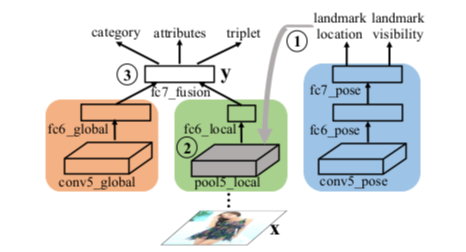
\includegraphics[width=10cm]{images/fashionnet-architecture.png} 
\centering
\caption{FashionNet Architecture \cite{deepfashion}}
\label{architecture}
\end{figure}

However, since the only task we wish to perform in this project is in-shop retrieval and in the interest of making our model simpler, we decided to use an approach relying on only a feature network and use Euclidean distance to find similar vectors. Our feature network will consist of a ResNet50 model trained on the DeepFashion clothing classification benchmark using transfer learning. This feature network will convert images into a 512-dim feature vector. We will then query the database to retrieve images who's feature vector has minimum euclidean distance from the query feature vector. In initial testing thus far, the approach works well. We will continue updating the literature review as we experiment and make our model more accurate and robust.

%\cite{einstein} but wish the work was typeset in \LaTeX \cite{knuthwebsite}, e.g. by taking help from \cite{latexcompanion}.

\chapter{Software Requirement Specification (SRS)}
\label{chap:srs}
This chapter provides detailed specifications of the system under development.

\section{Functional Requirements}

This section describes each function/feature provided by our system. These functions are logically grouped into modules based on their purpose/users/mode of operations etc (as per our system):
\begin{outline}
  \subsection{Web Application}
  \1 Allows customers to upload a photo of an outfit.
  \1 Displays constituent items of uploaded outfit.
  \1 Allows customers to click on a constituent item and view items identical/similar to it.
  \1 Allows customers to click on an item and open it's product page.
  \1 Displays item title, description, price, photos and sizes on product page.
  \1 On the product page, displays recommendations for similar products, as received from the recommendation engine.
  \1 On the product page, displays recommendations for complementary products, as received from the recommendation engine.
  \1 Allows customer to add item to cart.
  \1 Allows new customers to sign-up.
  \1 Allows returning customers to login.
  \1 Saves user history to database.
  \1 For existing customers with a user history: Displays recommendations based on user history, as received from the recommendation engine, on the home page.
  \1 For existing customers with a user history: Displays recommendations based on user history, as received from the recommendation engine, on product pages.
  \1 For new customers or existing customers without user history: Displays items currently trending on the store, on the home page.
  \1 Admin has exclusive access to an admin panel that allows them to add, remove and modify items on the website. 
  \1 Admin can view customer activity.
\end{outline}
\begin{outline}
  \subsection{Recommendation Engine}
  The engine can be roughly compartmentalized as follows:
  \1 On uploaded photo, calls feature extraction model and performs multiple object detection. To bounding boxes of each individual piece of clothing in the outfit.
  \1 Crops each bounding box in image and returns them. Each bounding box represents an article of clothing.
  \1 Upon receiving which bounding box has been selected by the user, it passes that to nearest neighbour model. Returns ids of n closest neighbours of that item from the database and ids of n best complimentary items.
\end{outline}
\begin{outline}
  \subsection{Database}
  \1 Should store id, title, price, description, sizes, category and tags for each item.
  \1 Should store user and admin account information.
  \1 Should store user profile information, including past logs, search history, purchase history, as well as other related actions.
\end{outline}
\begin{outline}
  \subsection{Web Scraper}
  \1 Crawl local fashion stores `Furor', `Export Leftovers', `J.', `Zellbury', etc.
  \1 For each item of men's clothing on the store, save the photo, description and price locally.
  \1 Add timed cron job functionality so that the database can be verified and kept up to date without discrepancies.
\end{outline}

\section{Non-functional Requirements}

\subsection{Performance Requirements}

\begin{itemize}
    \item High performance of the computer on which the server is hosted is needed to cater to thousands of users. 
    
    \item Fetching the dashboard to view information and recommended outfits shall take no longer than 5 seconds.
\end{itemize}

\subsection{Safety Requirements}
\begin{itemize}
    \item The system must not halt or lag, especially during the update time and must not go down under high traffic. In order to ensure safety of the server, it is suggested that it is hosted on two computers - one kept as a backup.
\end{itemize}

\subsection{Security Requirements}
\begin{itemize}
    \item It must be ensured that only the authorized admins, with valid user credentials, have access to the data of the users in order to ensure user privacy. 
    
    \item The system will use databases from authentic sources and fashion stores.
\end{itemize}

\subsection{User Interface}
\begin{itemize}
    \item The UI/UX flow needs to be intuitive as well as modern. 
\end{itemize}

\subsection{Error Handling}
\begin{itemize}
    \item The system prevents data loss by carefully handling all expected and non-expected errors. 
\end{itemize}

\section{External Interfaces}

\subsection{User Interfaces}

\subsubsection{Customer Interface}

\FloatBarrier
\begin{outline}
  \1 Homepage
  
  This interface would be visible to all the users and would lead to multiple other interfaces such as Login, Clothing categories, User profile, etc. This is shown in \autoref{gui:home}.


    
  \1 Registration
  
  This page allows a new user to create an account by filling the mandatory fields of 'User Name', 'Email', 'Password' and 'Confirmed Password'. In case of valid details, user will be able to login, else they are redirected to the same sign-up page. This is shown in \autoref{gui:sign}.


    
  \1 Login
  
  This interface enables user to log into the system using valid credentials, and redirects him/her to the homepage if the credentials are validated, otherwise an error message is displayed. Login interface requires 'User Name' and 'Password' as the mandatory fields. This is shown in \autoref{gui:login}.


  \1 Profile
  
  A user would be able to see this interface if they have created an account and are logged into the system. This interface would enable them to view their account details and their previously searched/recommended outfit statistics. This is shown in \autoref{gui:profile}.


  \1 Product Display
  
  A user would be able to see different product categories along with the details of each product available in the stock. This is shown in \autoref{gui:product1}, \autoref{gui:product2}, and \autoref{gui:product3}.
  

  
  
  \1 Upload Image
  
  A user would be able to upload image of his/her clothing item, in order to search visually similar or complementary items. This is shown in \autoref{gui:upload1} and \autoref{gui:upload2}.
  


  \1 Cart
  
  This interface enables a user to view their selected recommended outfits and would show them the third-party referral links to each of their chosen outfits. This is shown in \autoref{gui:cart}.
  

  \1 Our Brands

  This interface would display the vendors and the third-party brands with whom we will partner up with. A user would be able to retrieve products based on any specific store from these brands. This is shown in \autoref{gui:brands}. 
  
 \end{outline}
 
 \subsubsection{System Admin Interface}
 \begin{outline}
   \1 Login
   
   Using the login interface, the system admin would log into the system using his/her valid credentials and would be redirected to the system admin homepage. This is shown in \autoref{gui:login}.
   
   \1 Homepage
   
   This interface enables the system admin to get redirected to multiple other navigation pages such as User Details, and Vendor details. This is shown in \autoref{gui:home}.
   
   \1 User Details
   
   This interface contains user details such as their personal information, their cart details and their preferred trend statistics. This is shown in \autoref{gui:profiles1} and \autoref{gui:profiles2}.
   
   \1 Vendor Details
   
   This interface allows the system admin to view details of the vendor such as the trends of their most recommended outfits, new additions to their outfit database, top users visiting the respective vendor page (using the referral link). This is shown in \autoref{gui:vendor1} and \autoref{gui:vendor2}.
 \end{outline}

\subsubsection{GUI Mockups}
\begin{figure}[H]
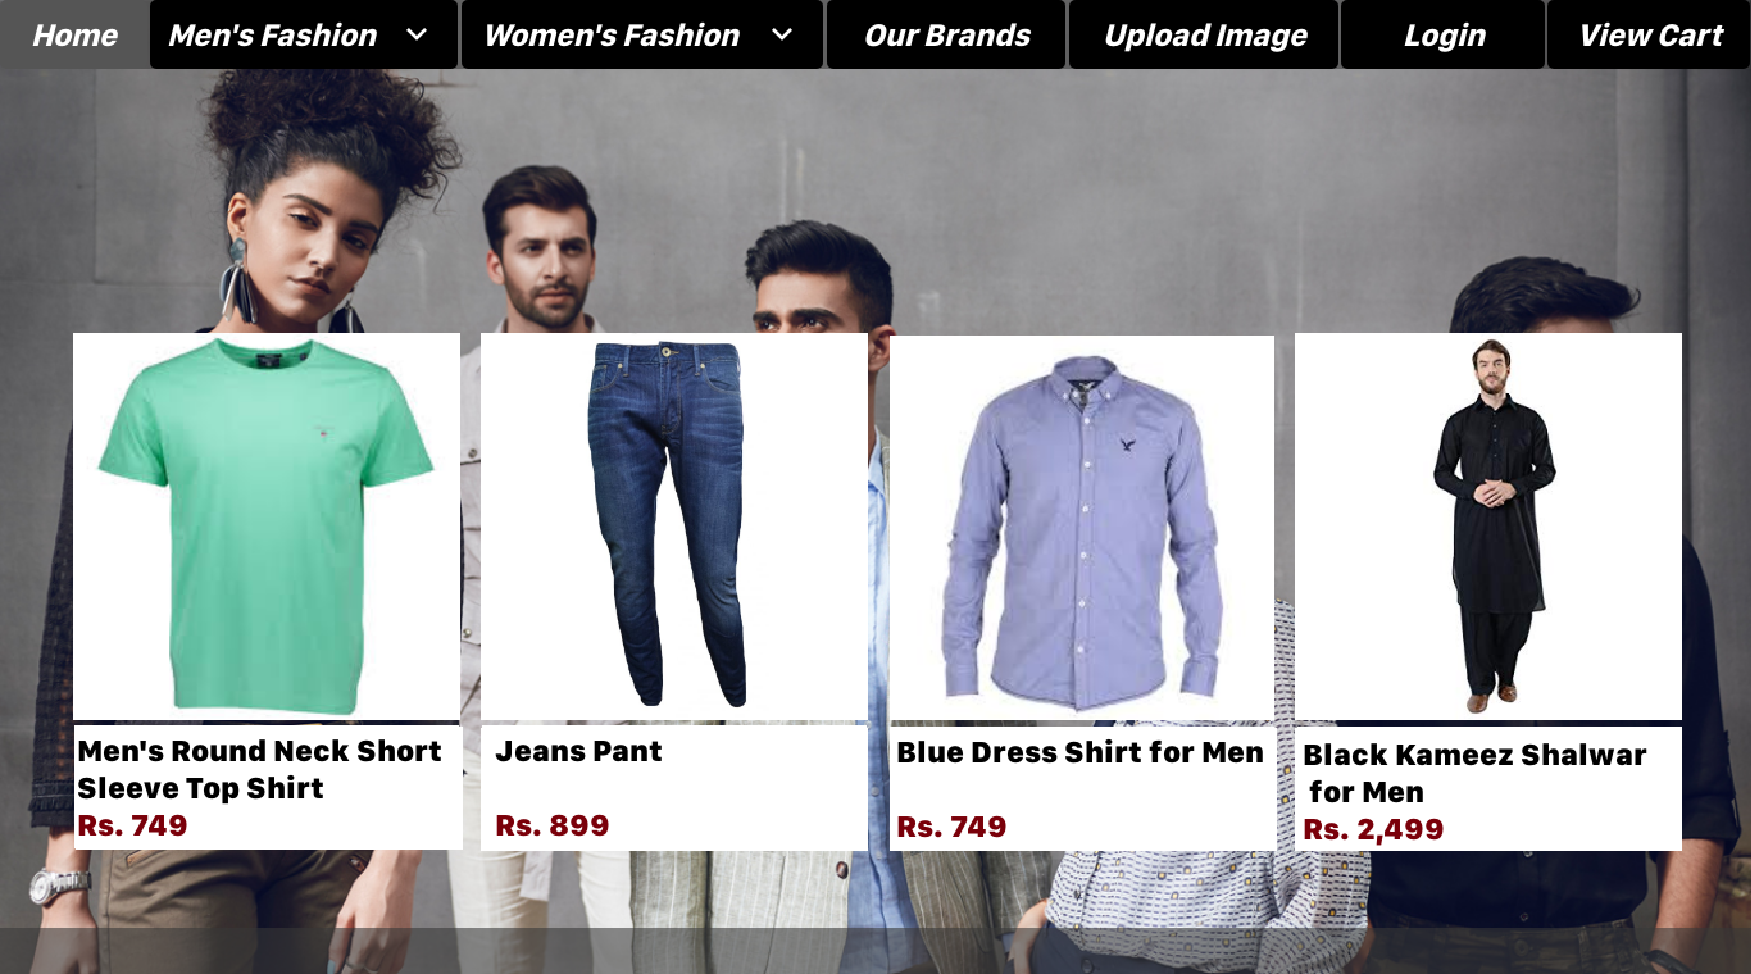
\includegraphics[width=15cm]{images/HomeScreen.pdf} 
\centering
\caption{Home Screen}
\label{gui:home}
\end{figure}

 \begin{figure}[H]
  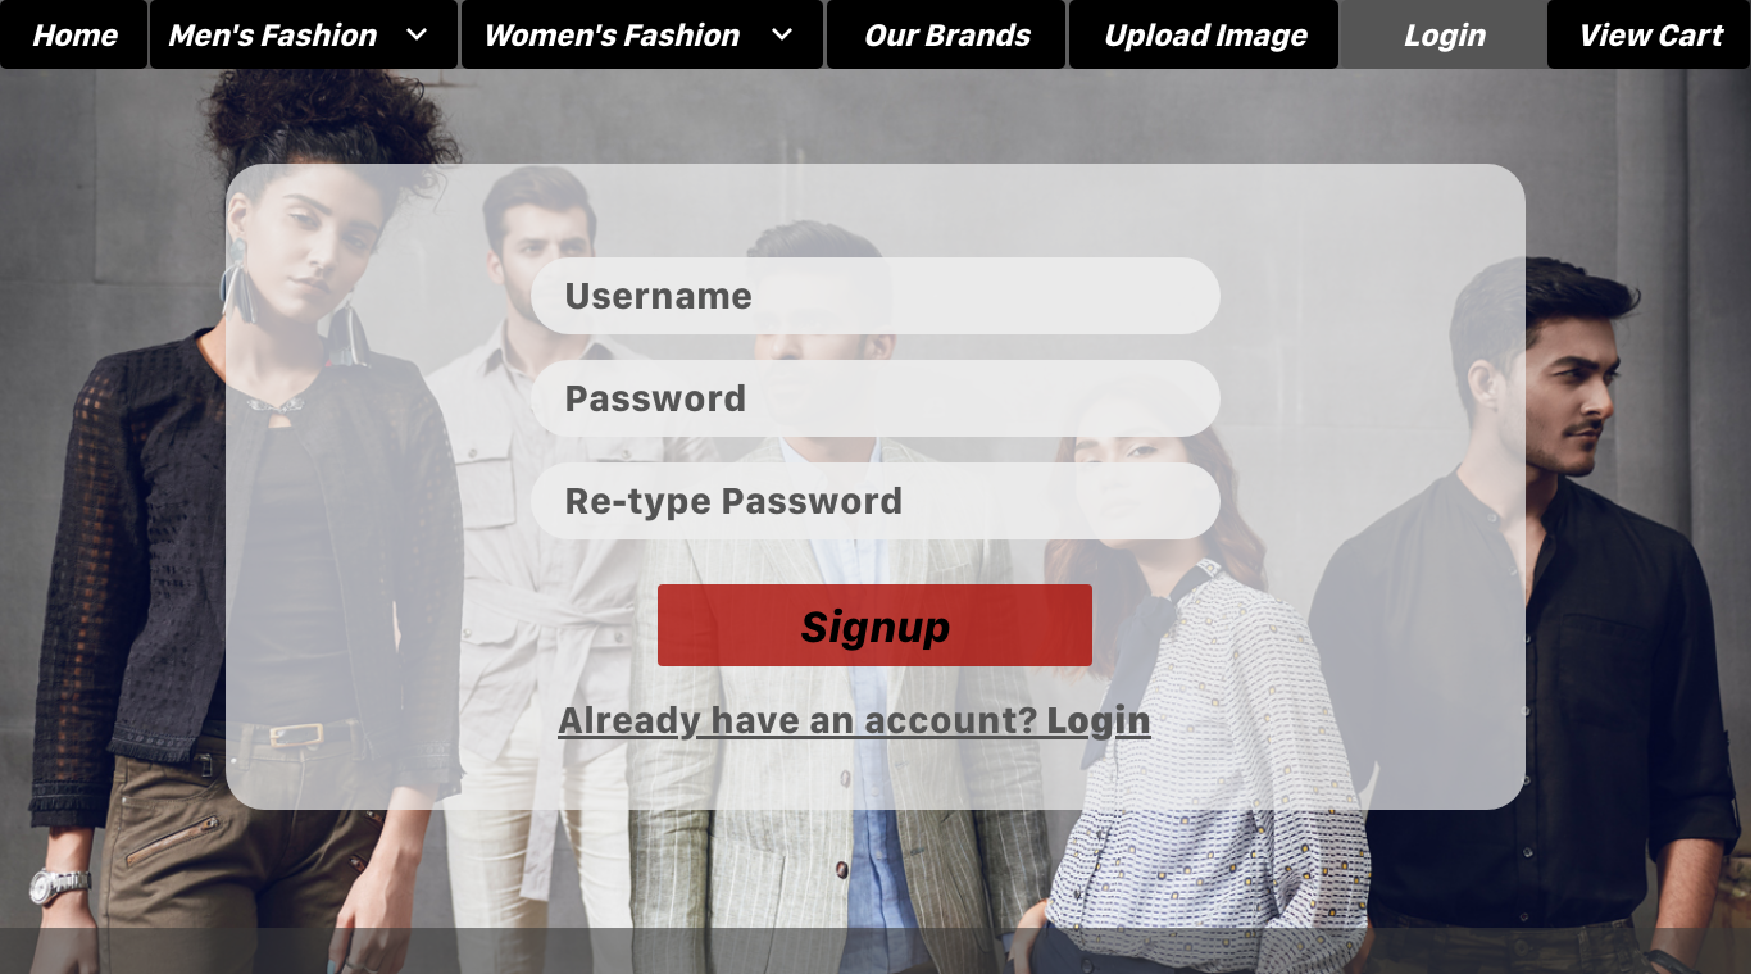
\includegraphics[width=15cm]{images/SignupScreen.pdf} 
  \centering
  \caption{Sign-up Screen}
  \label{gui:sign}
  \end{figure}

  \begin{figure}[!htb]
  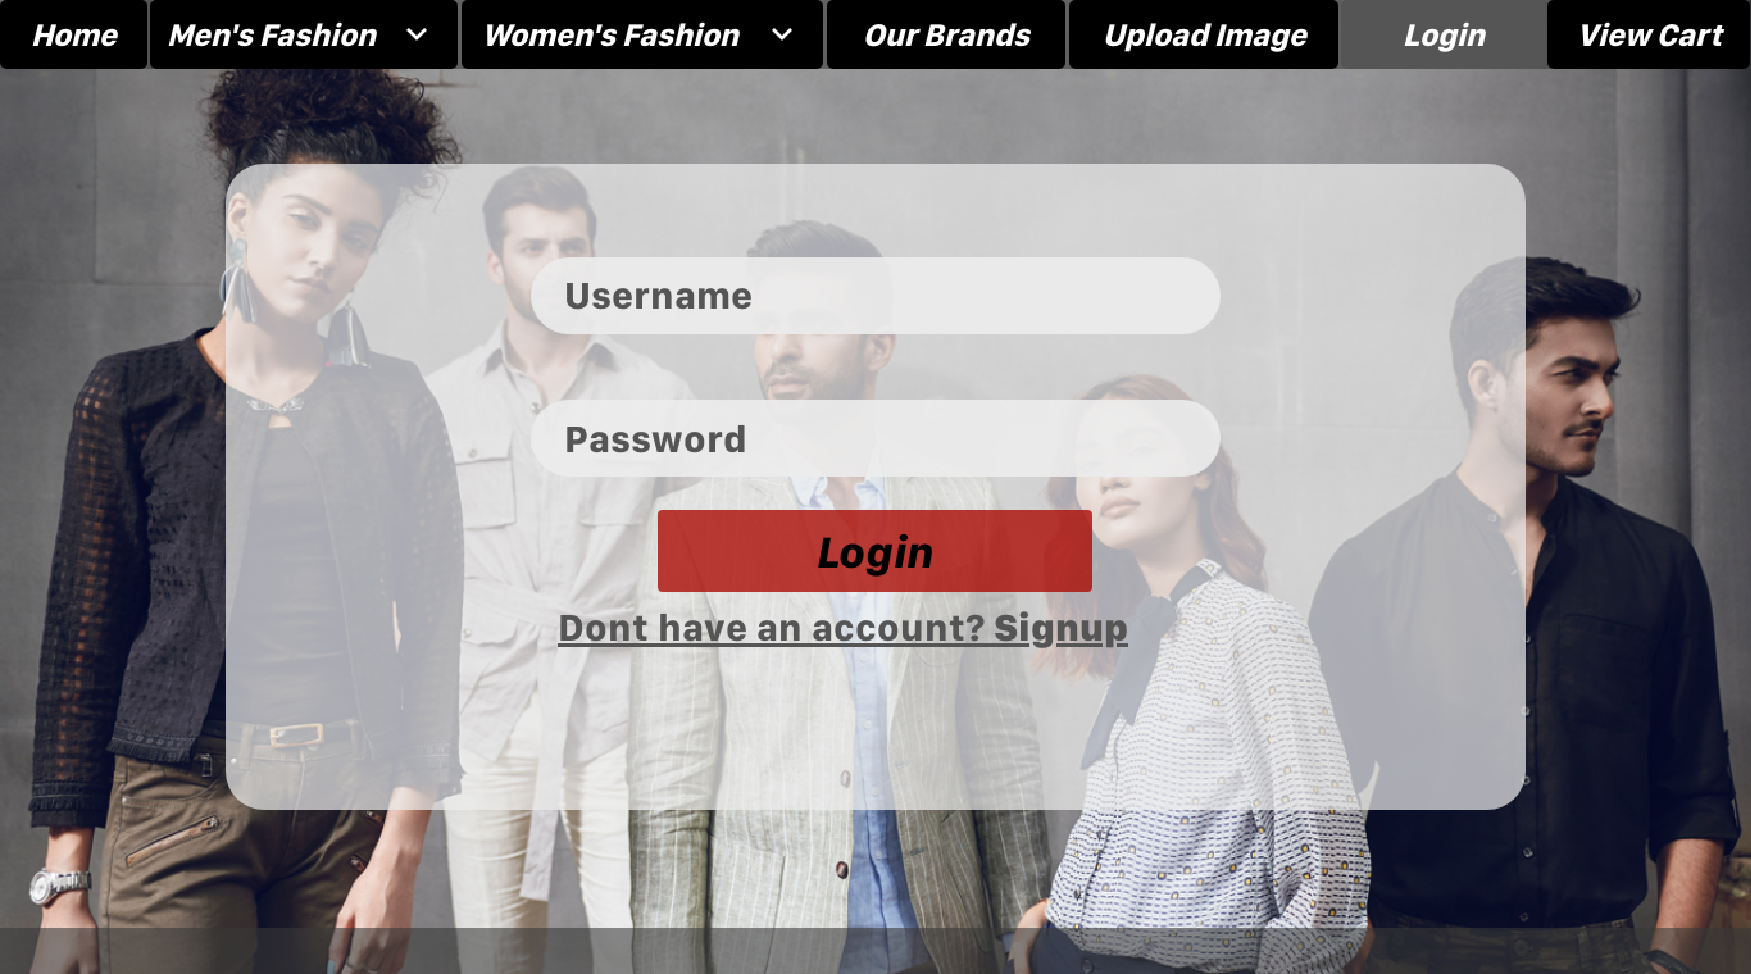
\includegraphics[width=15cm]{images/LoginScreen.pdf} 
  \centering
  \caption{Login Screen}
  \label{gui:login}
  \end{figure}

  \begin{figure}[H]
  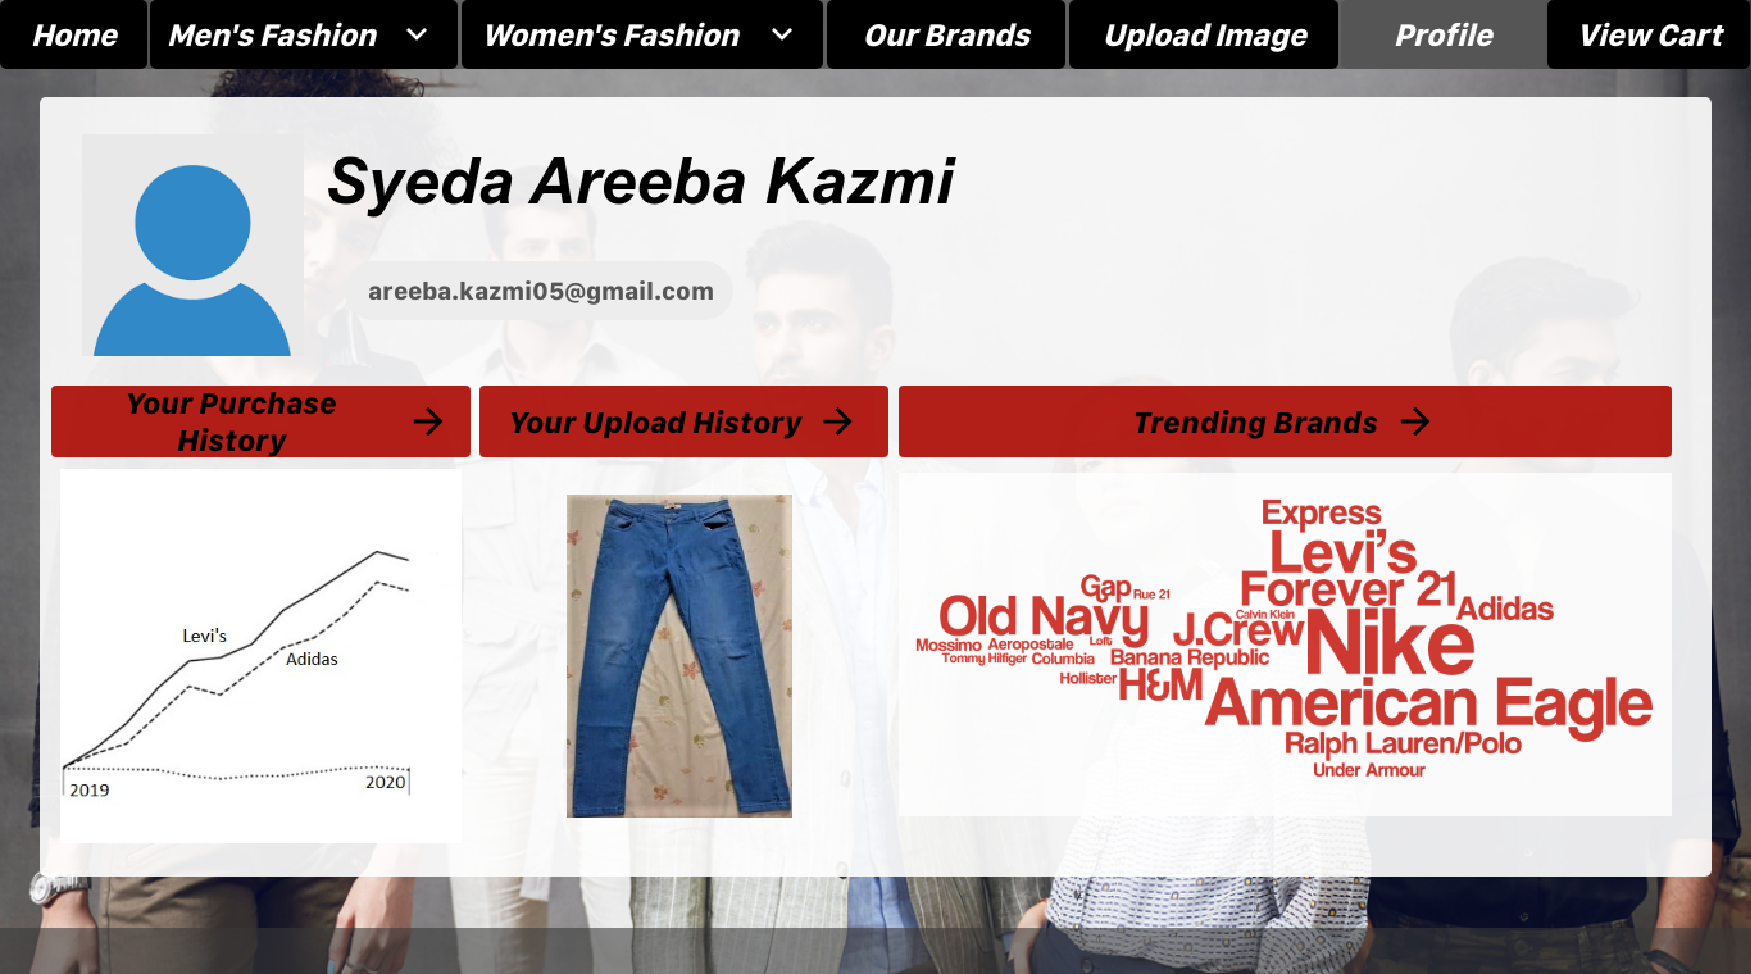
\includegraphics[width=15cm]{images/UserProfileScreen.pdf} 
  \centering
  \caption{User Profile Screen}
  \label{gui:profile}
  \end{figure}
  \begin{figure}[H]
  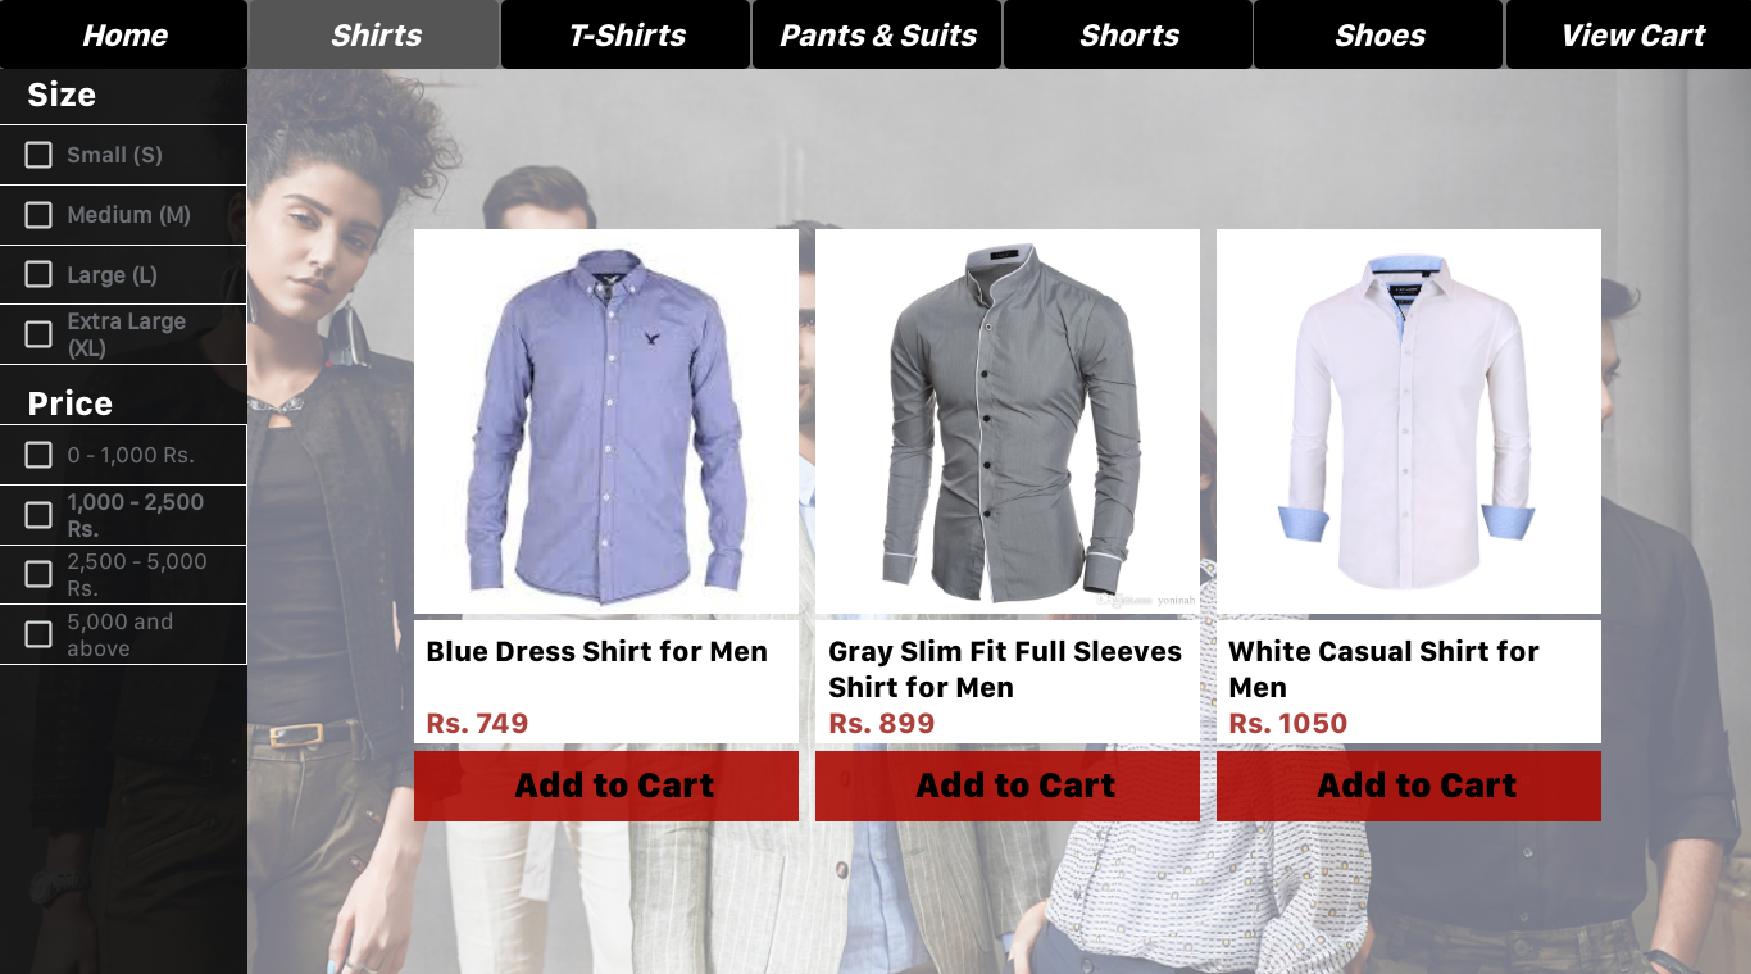
\includegraphics[width=15cm]{images/ShirtsScreen.pdf} 
  \centering
  \caption{Shirt Category Screen}
  \label{gui:product1}
  \end{figure}
  
  \begin{figure}[H]
  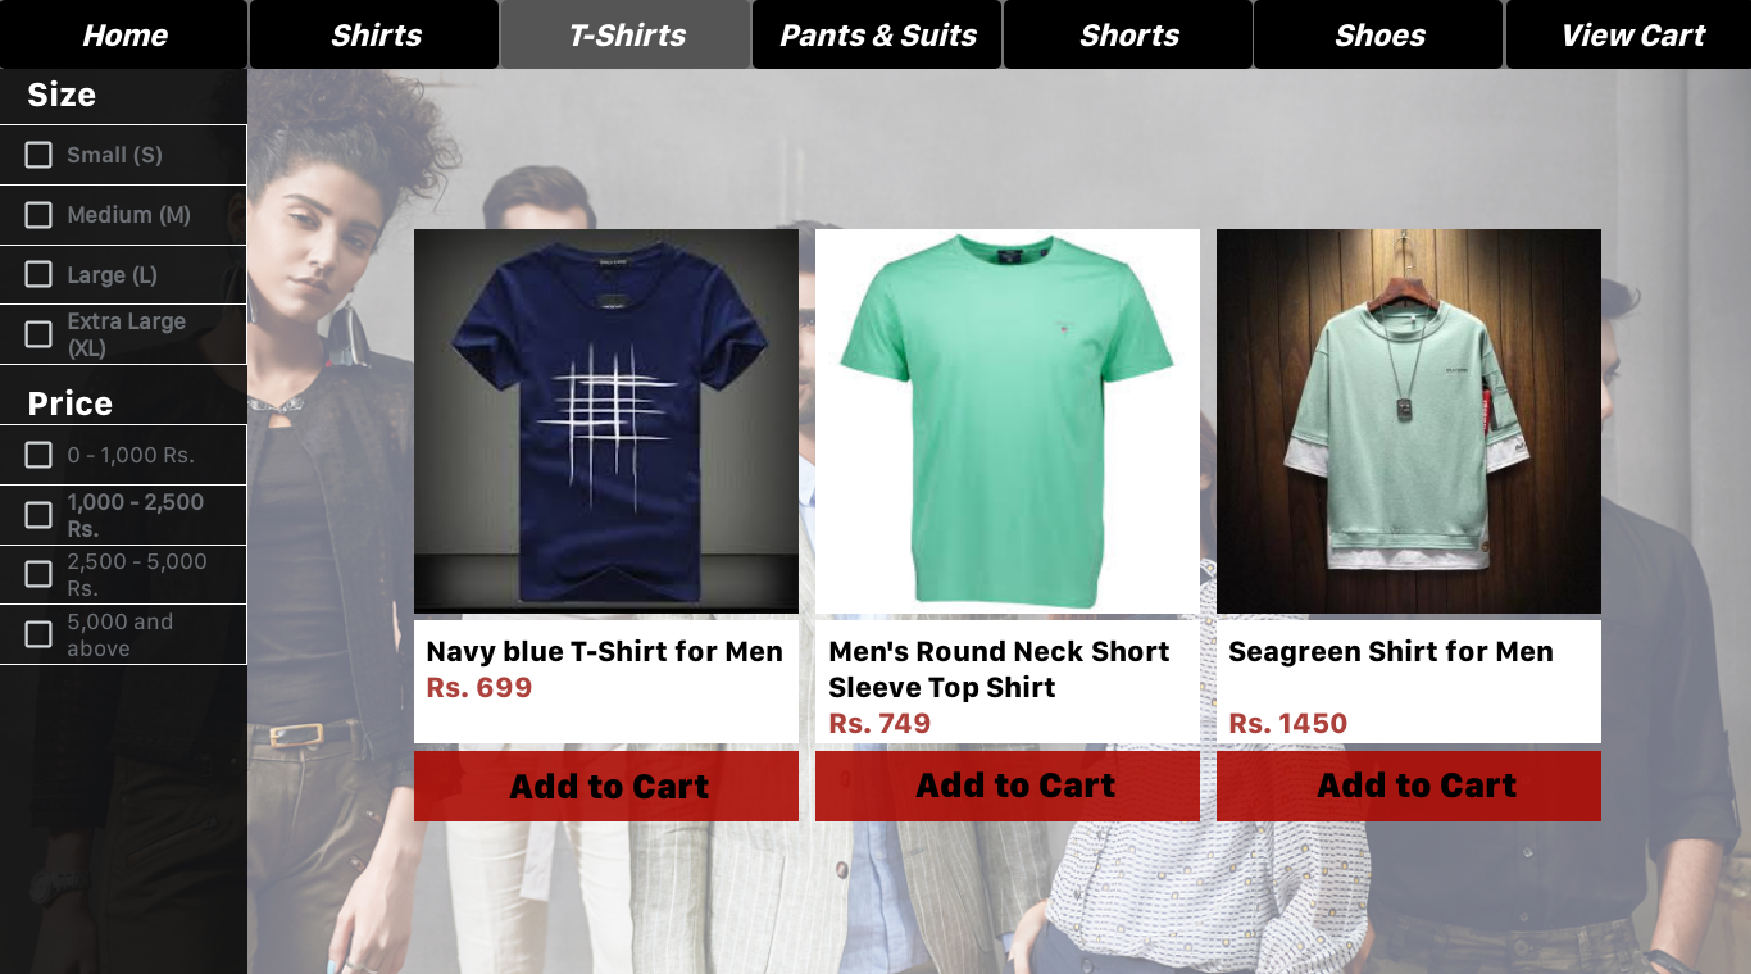
\includegraphics[width=15cm]{images/TShirtsScreen.pdf}
  \centering
  \caption{T-Shirt Category Screen}
  \label{gui:product2}
  \end{figure}
  
  \begin{figure}[H]
  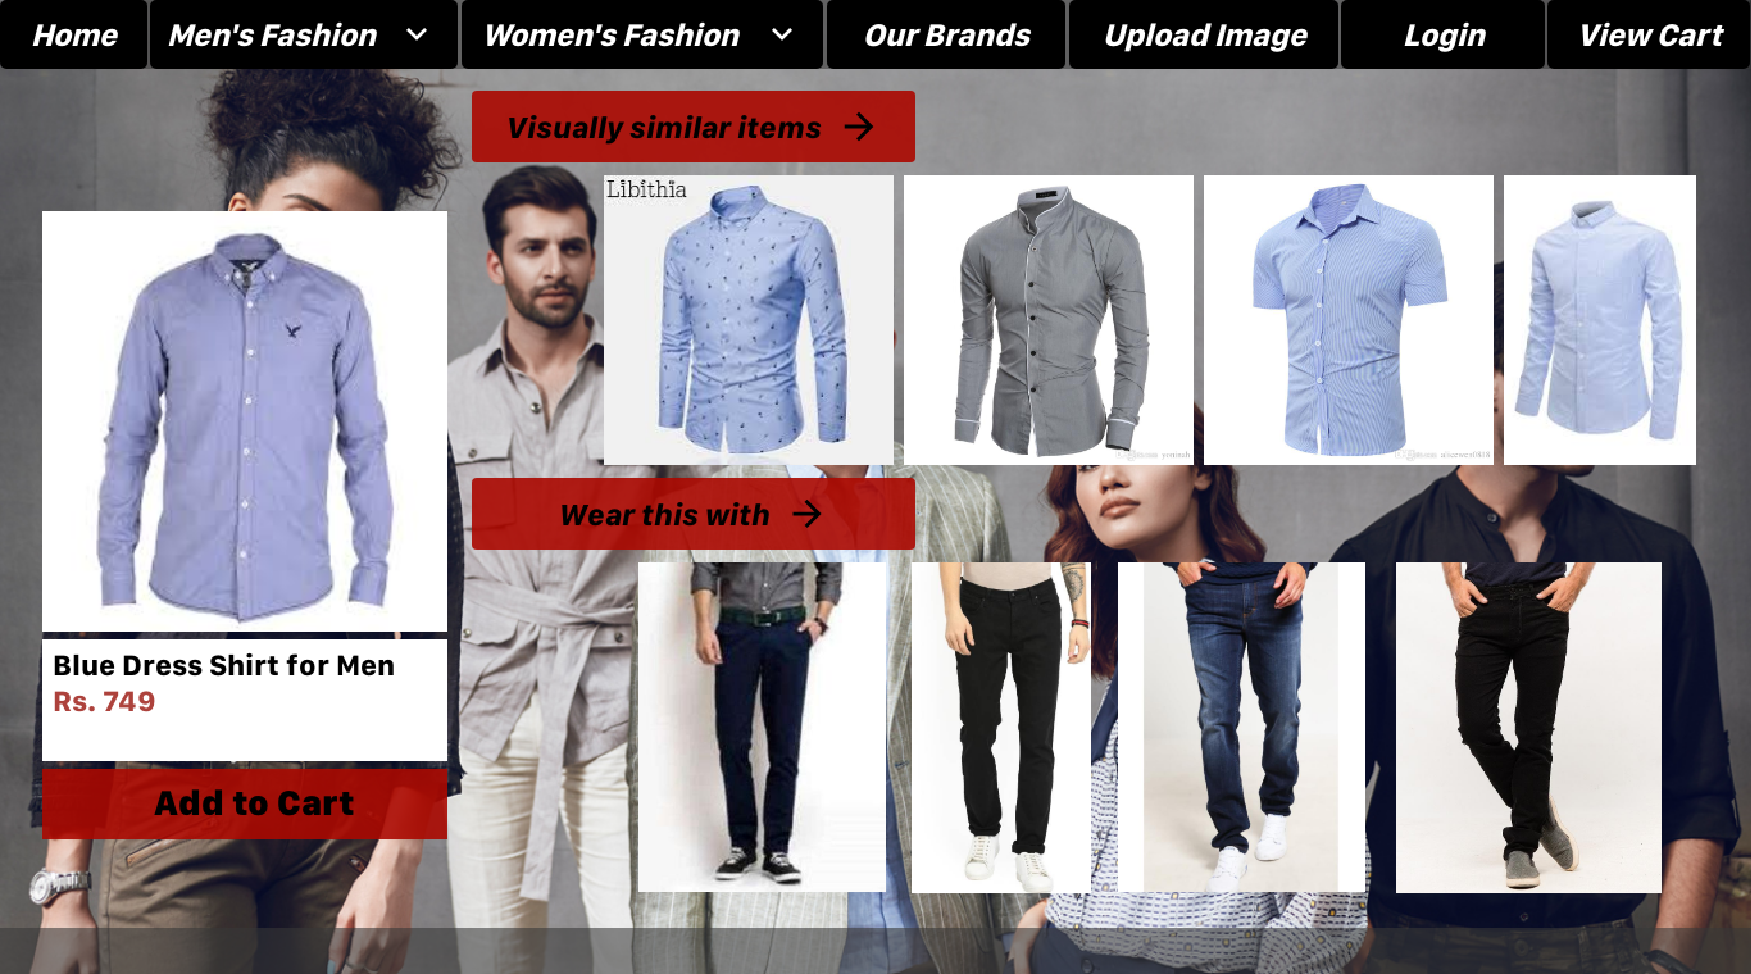
\includegraphics[width=15cm]{images/ProductDetailsScreen.pdf} 
  \centering
  \caption{Recommendation Screen 1.0}
  \label{gui:product3}
  \end{figure}
  \begin{figure}[H]
  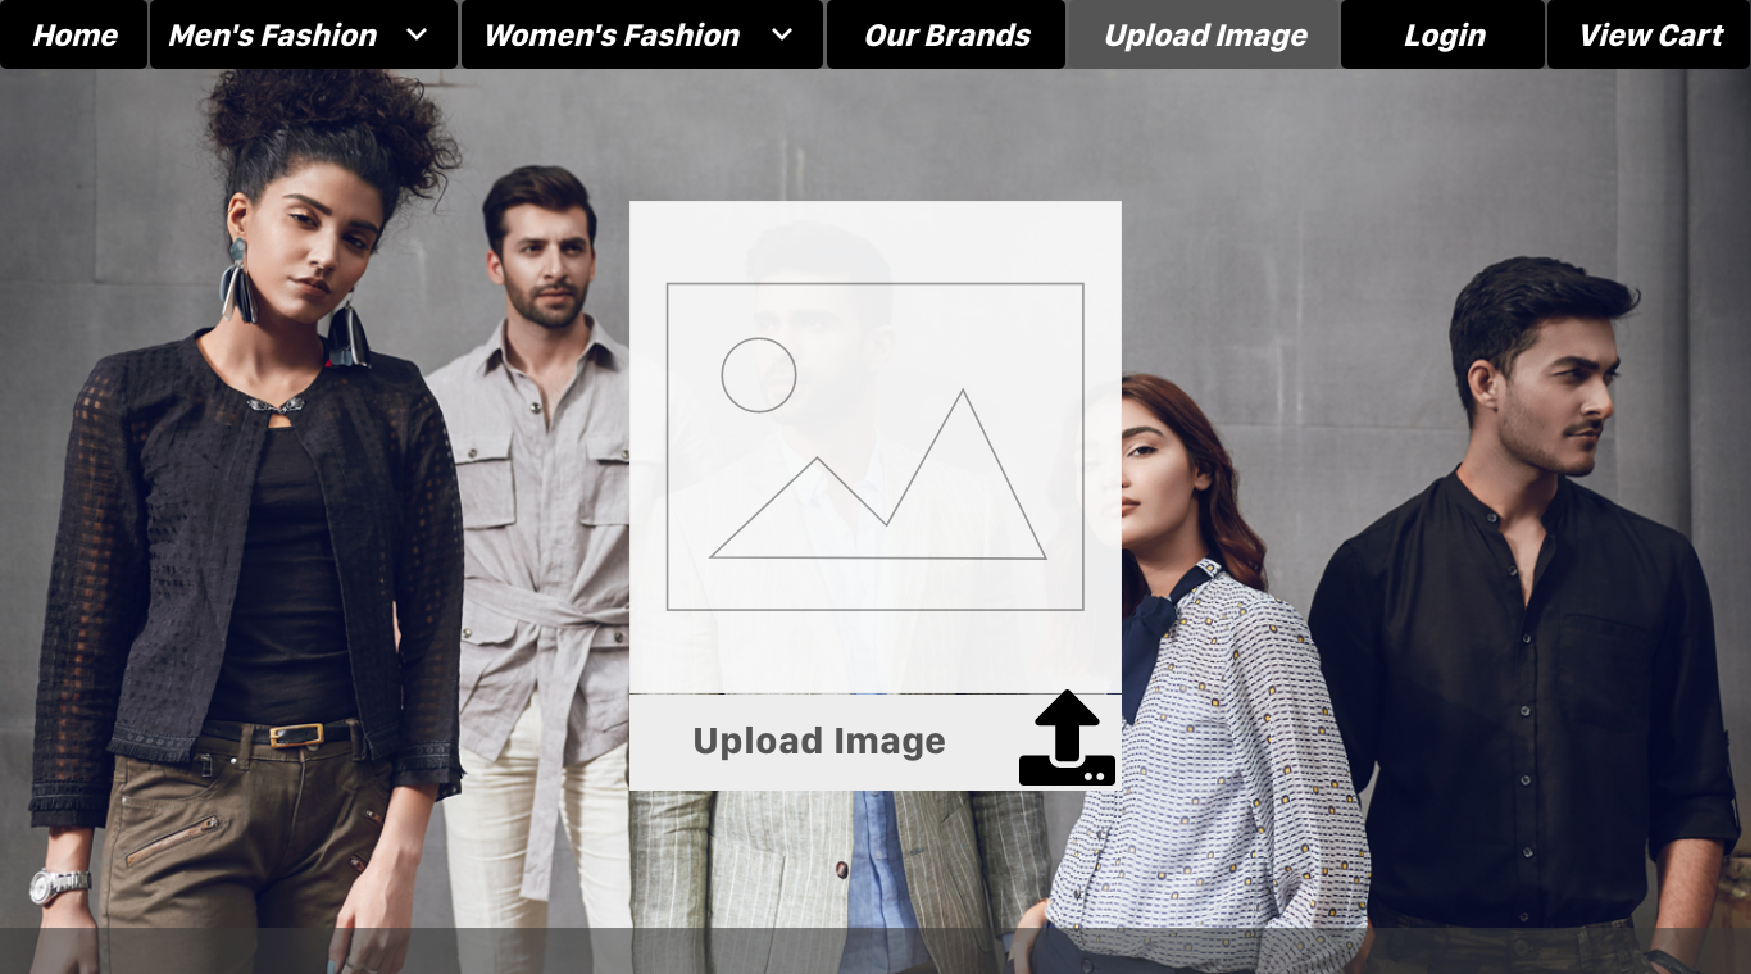
\includegraphics[width=15cm]{images/UploadImageScreen.pdf} 
  \centering
  \caption{Upload Image Screen}
  \label{gui:upload1}
  \end{figure}
  
  \begin{figure}[H]
  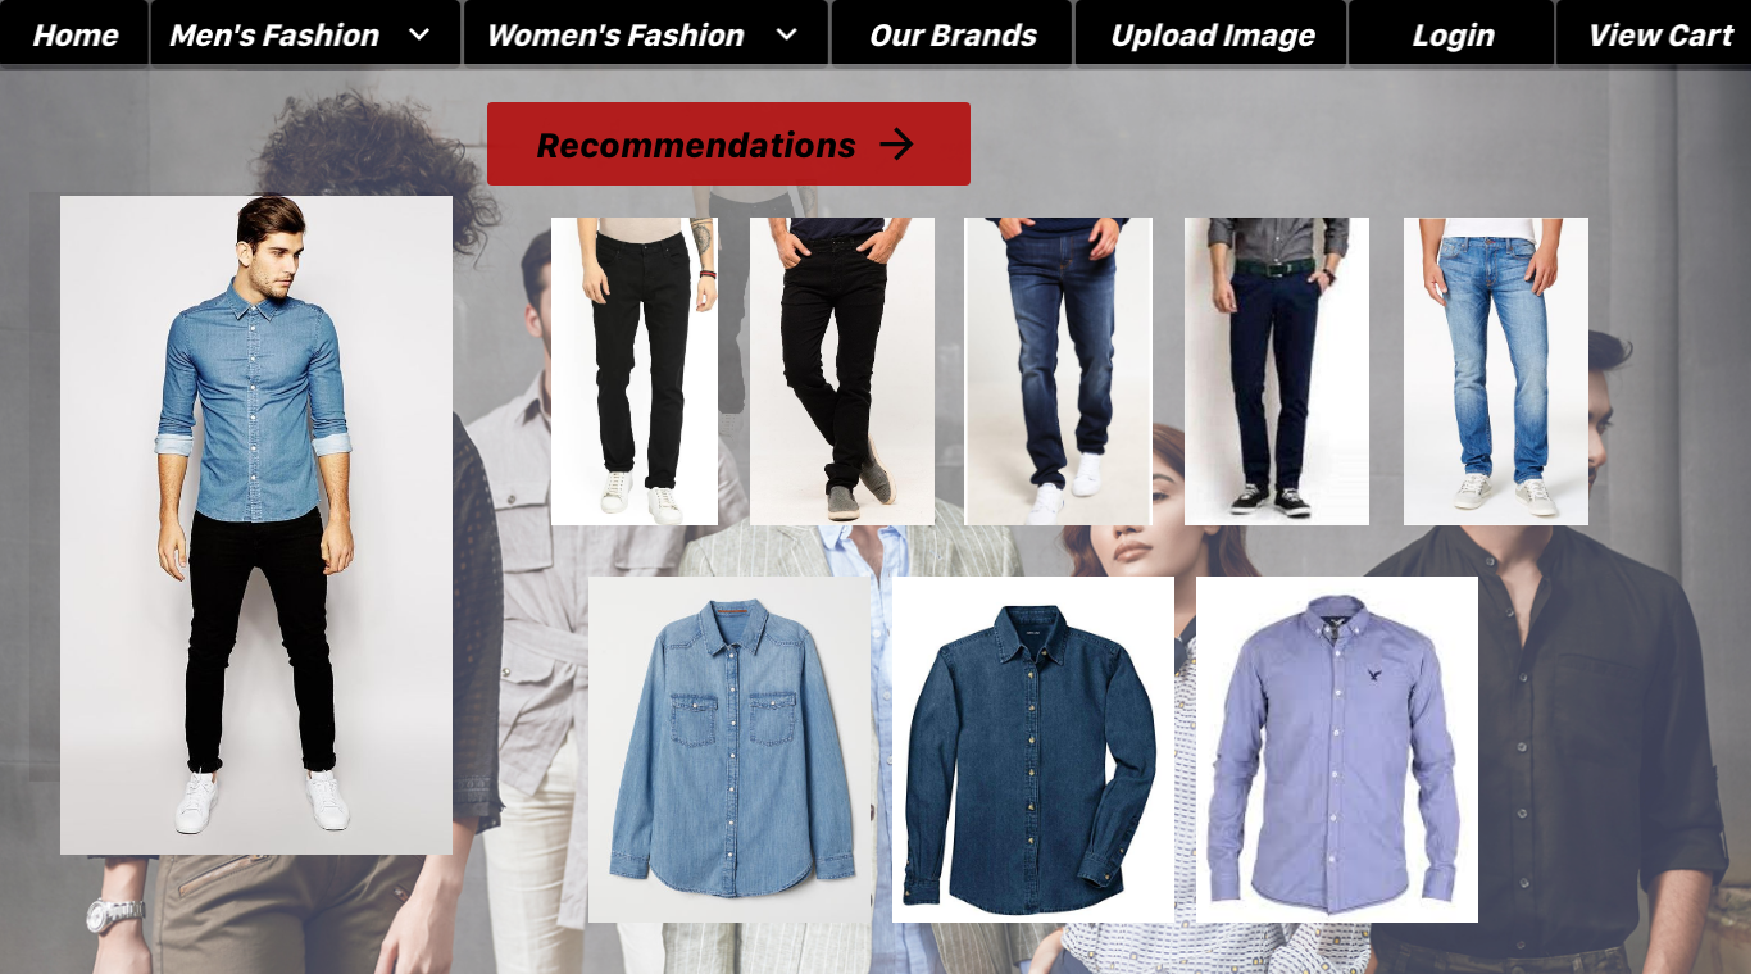
\includegraphics[width=15cm]{images/UploadedImagedetailsScreen.pdf} 
  \centering
  \caption{Recommendation Screen 2.0}
  \label{gui:upload2}
  \end{figure}

  \begin{figure}[H]
  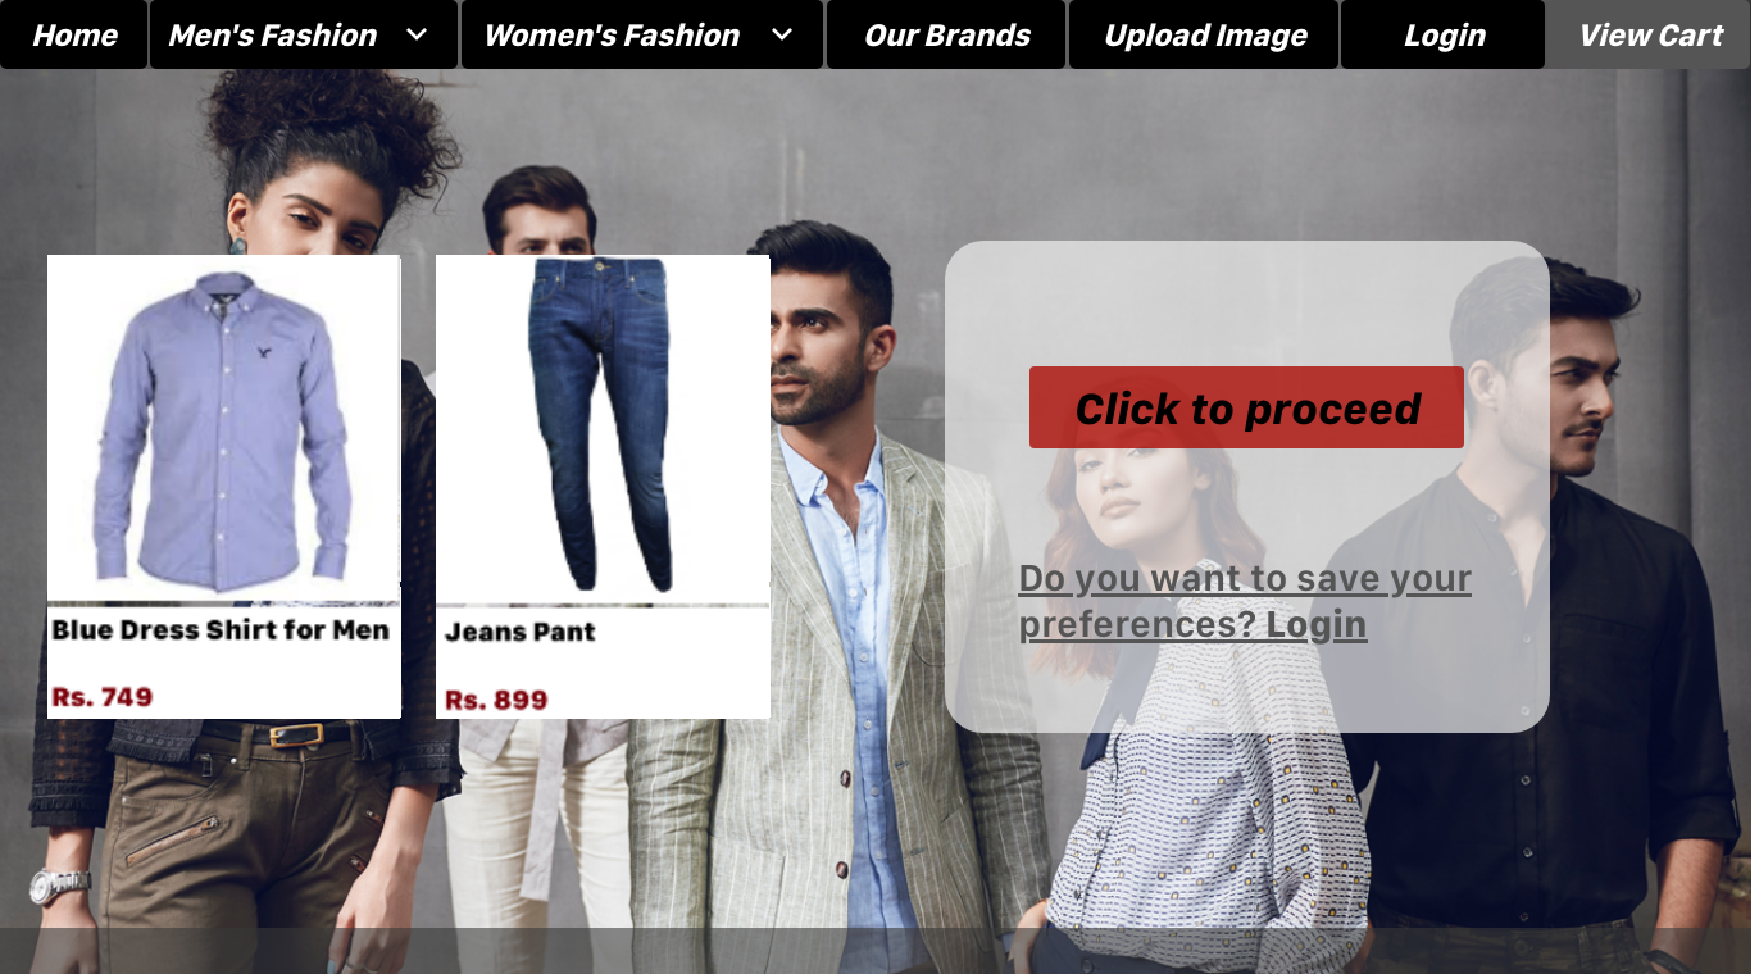
\includegraphics[width=15cm]{images/ViewCart.pdf} 
  \centering
  \caption{View Your Cart Screen}
  \label{gui:cart}
  \end{figure}

  \begin{figure}[H]
  
\includegraphics[width=15cm]{images/OurBrands.pdf} 
  \centering
  \caption{Partner Brands Screen}
  \label{gui:brands}
  \end{figure}

   \begin{figure}[H]
  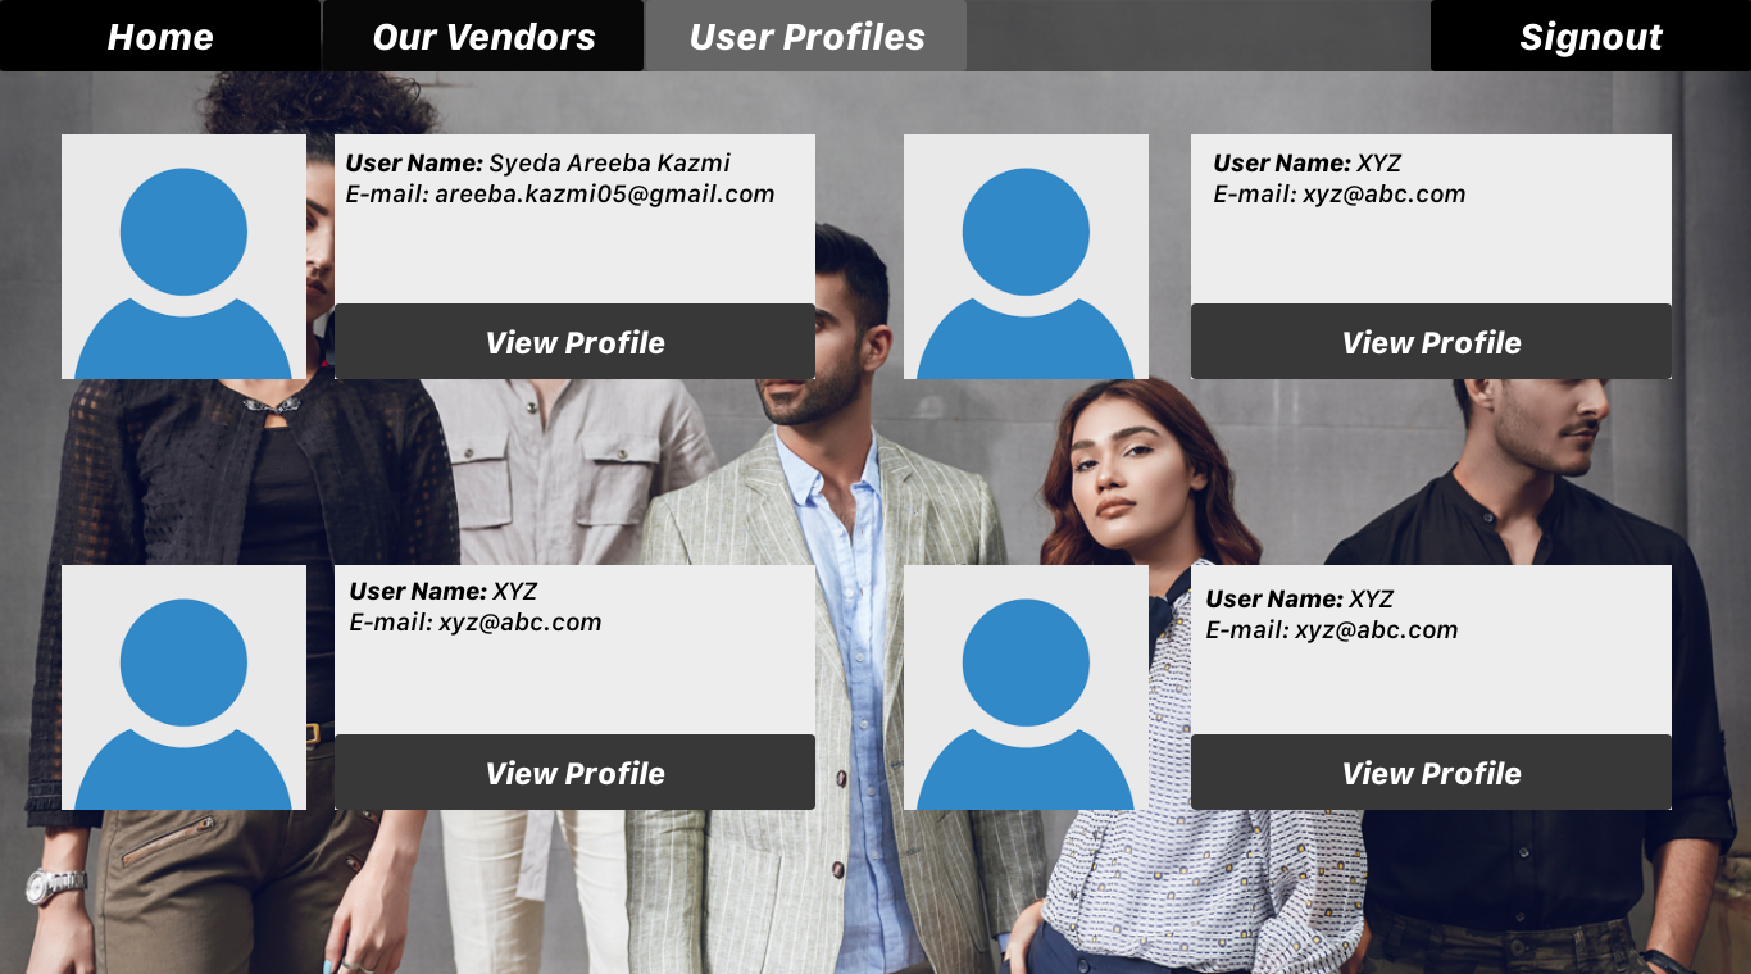
\includegraphics[width=15cm]{images/Profiles1.pdf} 
  \centering
  \caption{Admin-User Profiles Screen 1}
  \label{gui:profiles1}
  \end{figure}

   \begin{figure}[H]
  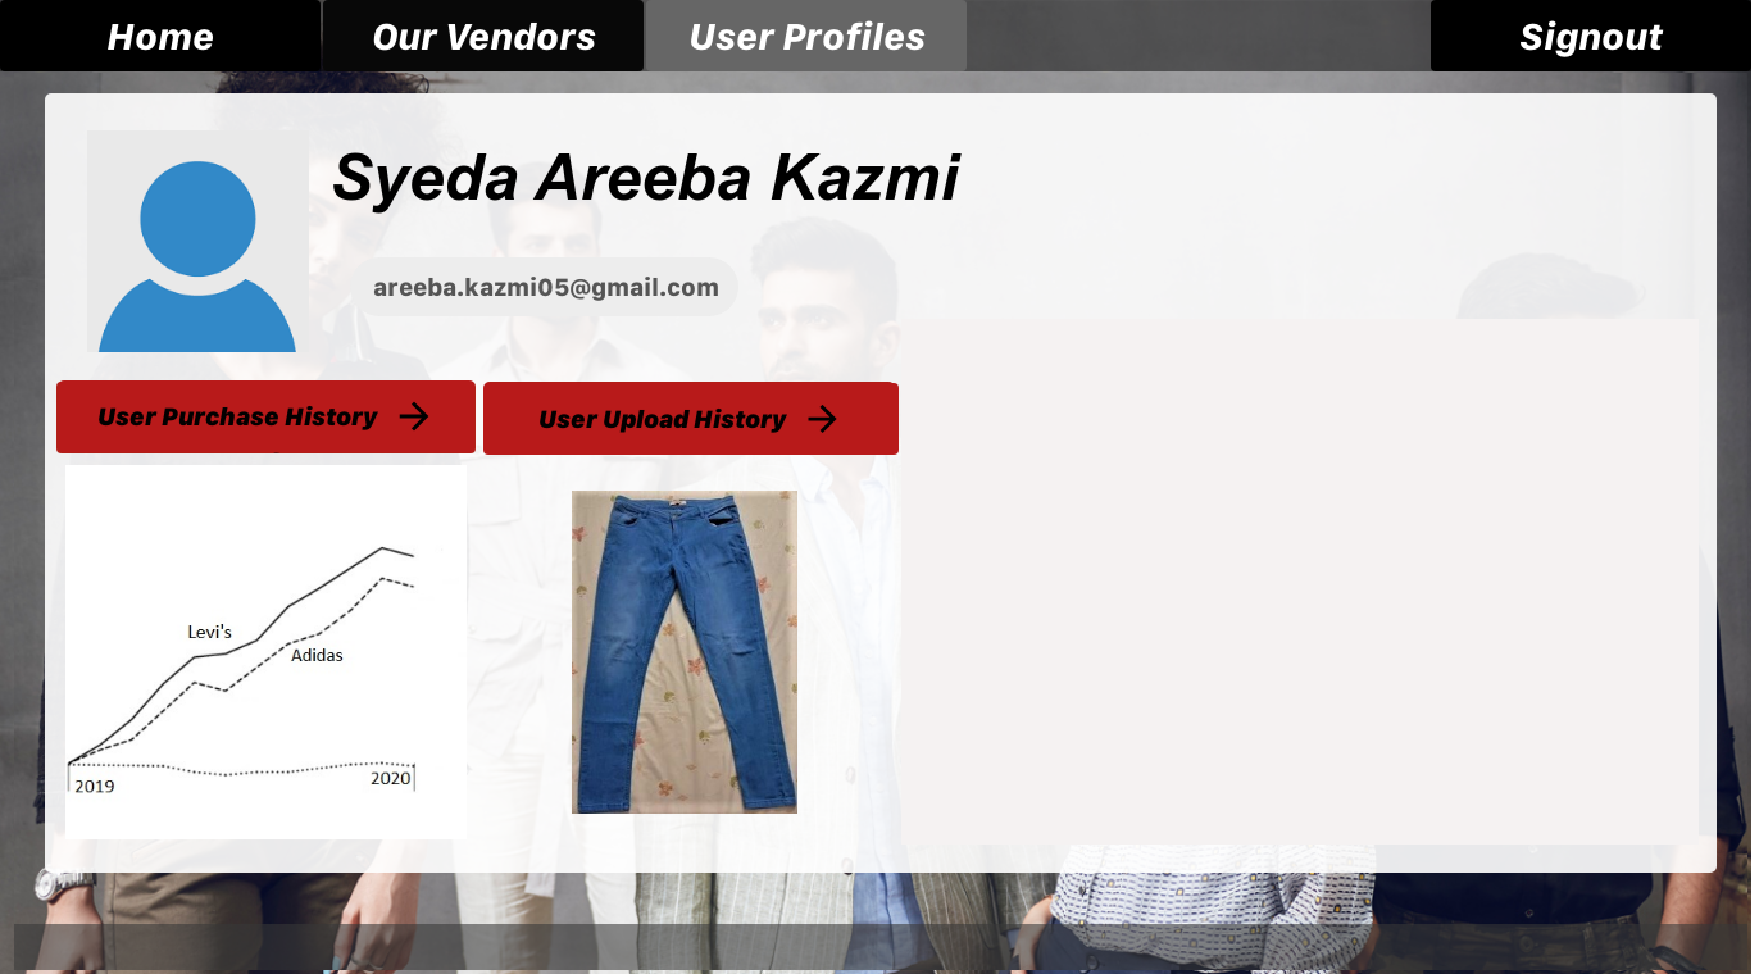
\includegraphics[width=15cm]{images/Profiles2.pdf} 
  \centering
  \caption{Admin-User Profiles Screen 1}
  \label{gui:profiles2}
  \end{figure}

   \begin{figure}[H]
  
\includegraphics[width=15cm]{images/VendorScreen1.pdf} 
  \centering
  \caption{Admin Vendors Screen 1}
  \label{gui:vendor1}
  \end{figure}

   \begin{figure}[H]
  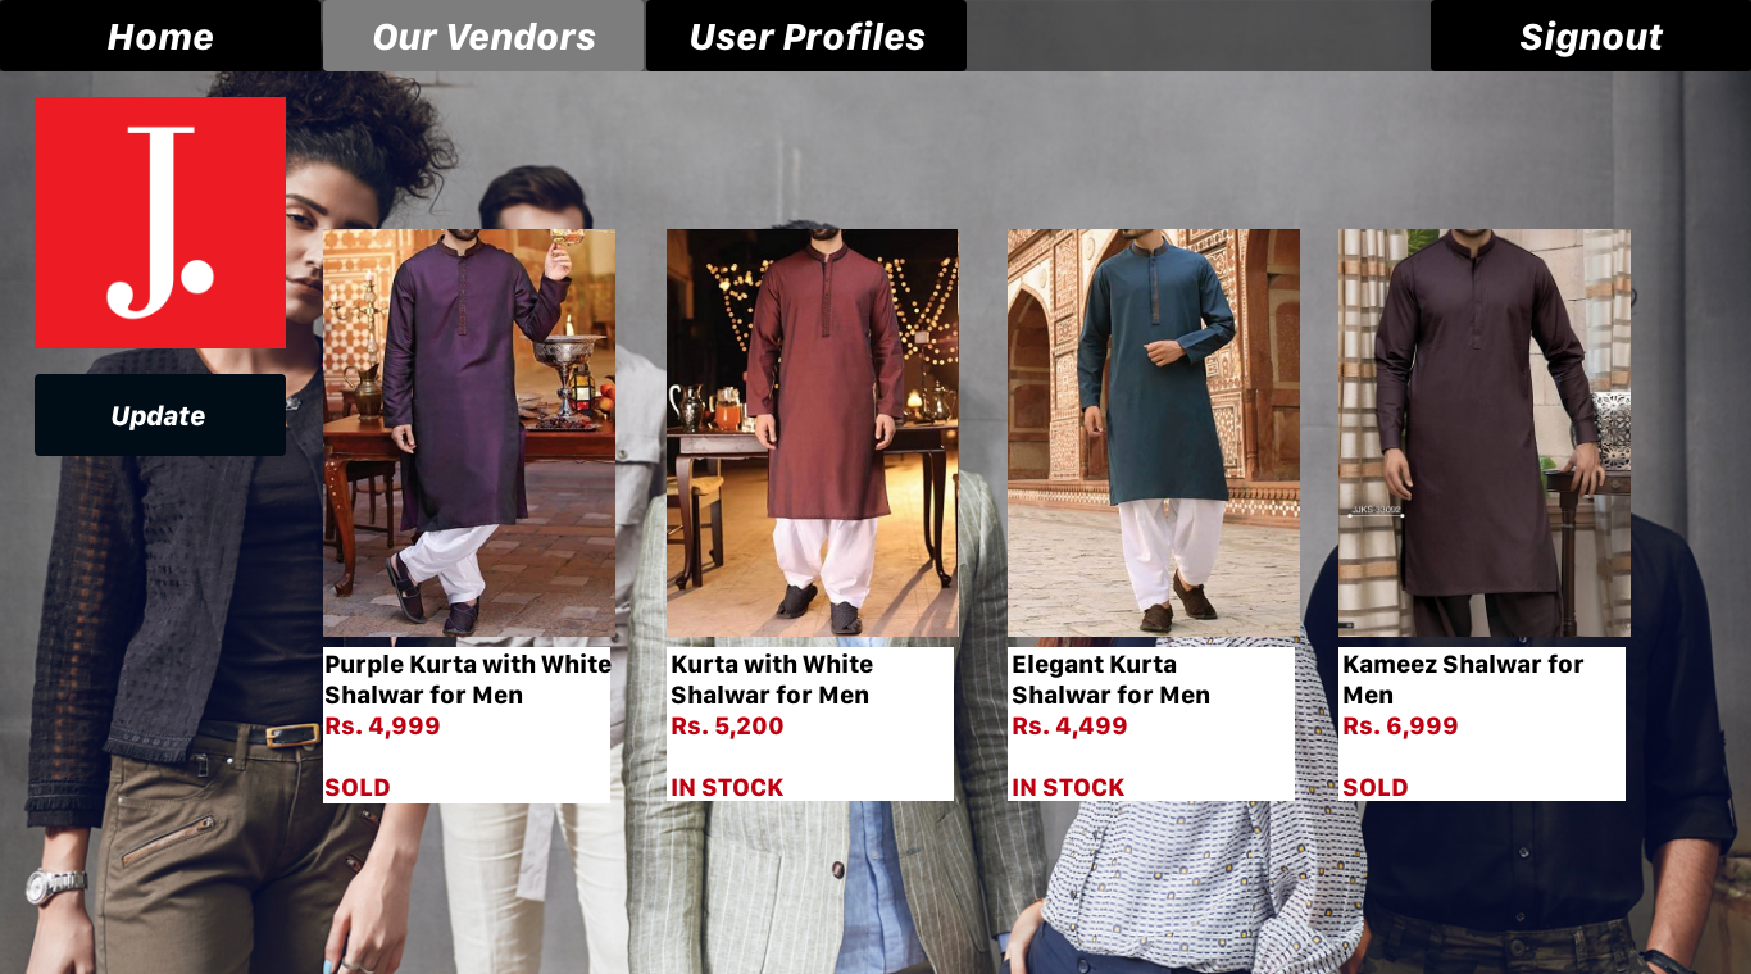
\includegraphics[width=15cm]{images/VendorScreen2.pdf} 
  \centering
  \caption{Admin Vendors Screen 2}
  \label{gui:vendor2}
  \end{figure}

\subsection{Application Program Interface (API)}
The system will be built using the Django framework at the server-end, and React.JS at the client-end (explained in detail in \autoref{srs:sysdiag}). We aim to use REST (Representational State Transfer) APIs, served through the Django REST framework, for all client-server communication since RESTful services as an architectural style would lead to our application being lightweight and scalable. However, since graph-based communication channels are gaining more popularity and adaptation rates in internet technologies these days, and for reasons summarized in \autoref{table:tech-api} ahead, our eventual goal is to establish an API based entirely off of GraphQL. So, for purposes of this web-application, our API will be written primarily as a RESTful service, but will be exposed to the client through a schema-first approach using a GraphQL wrapper. \autoref{api:diag} summarizes this.
\begin{figure}[H]
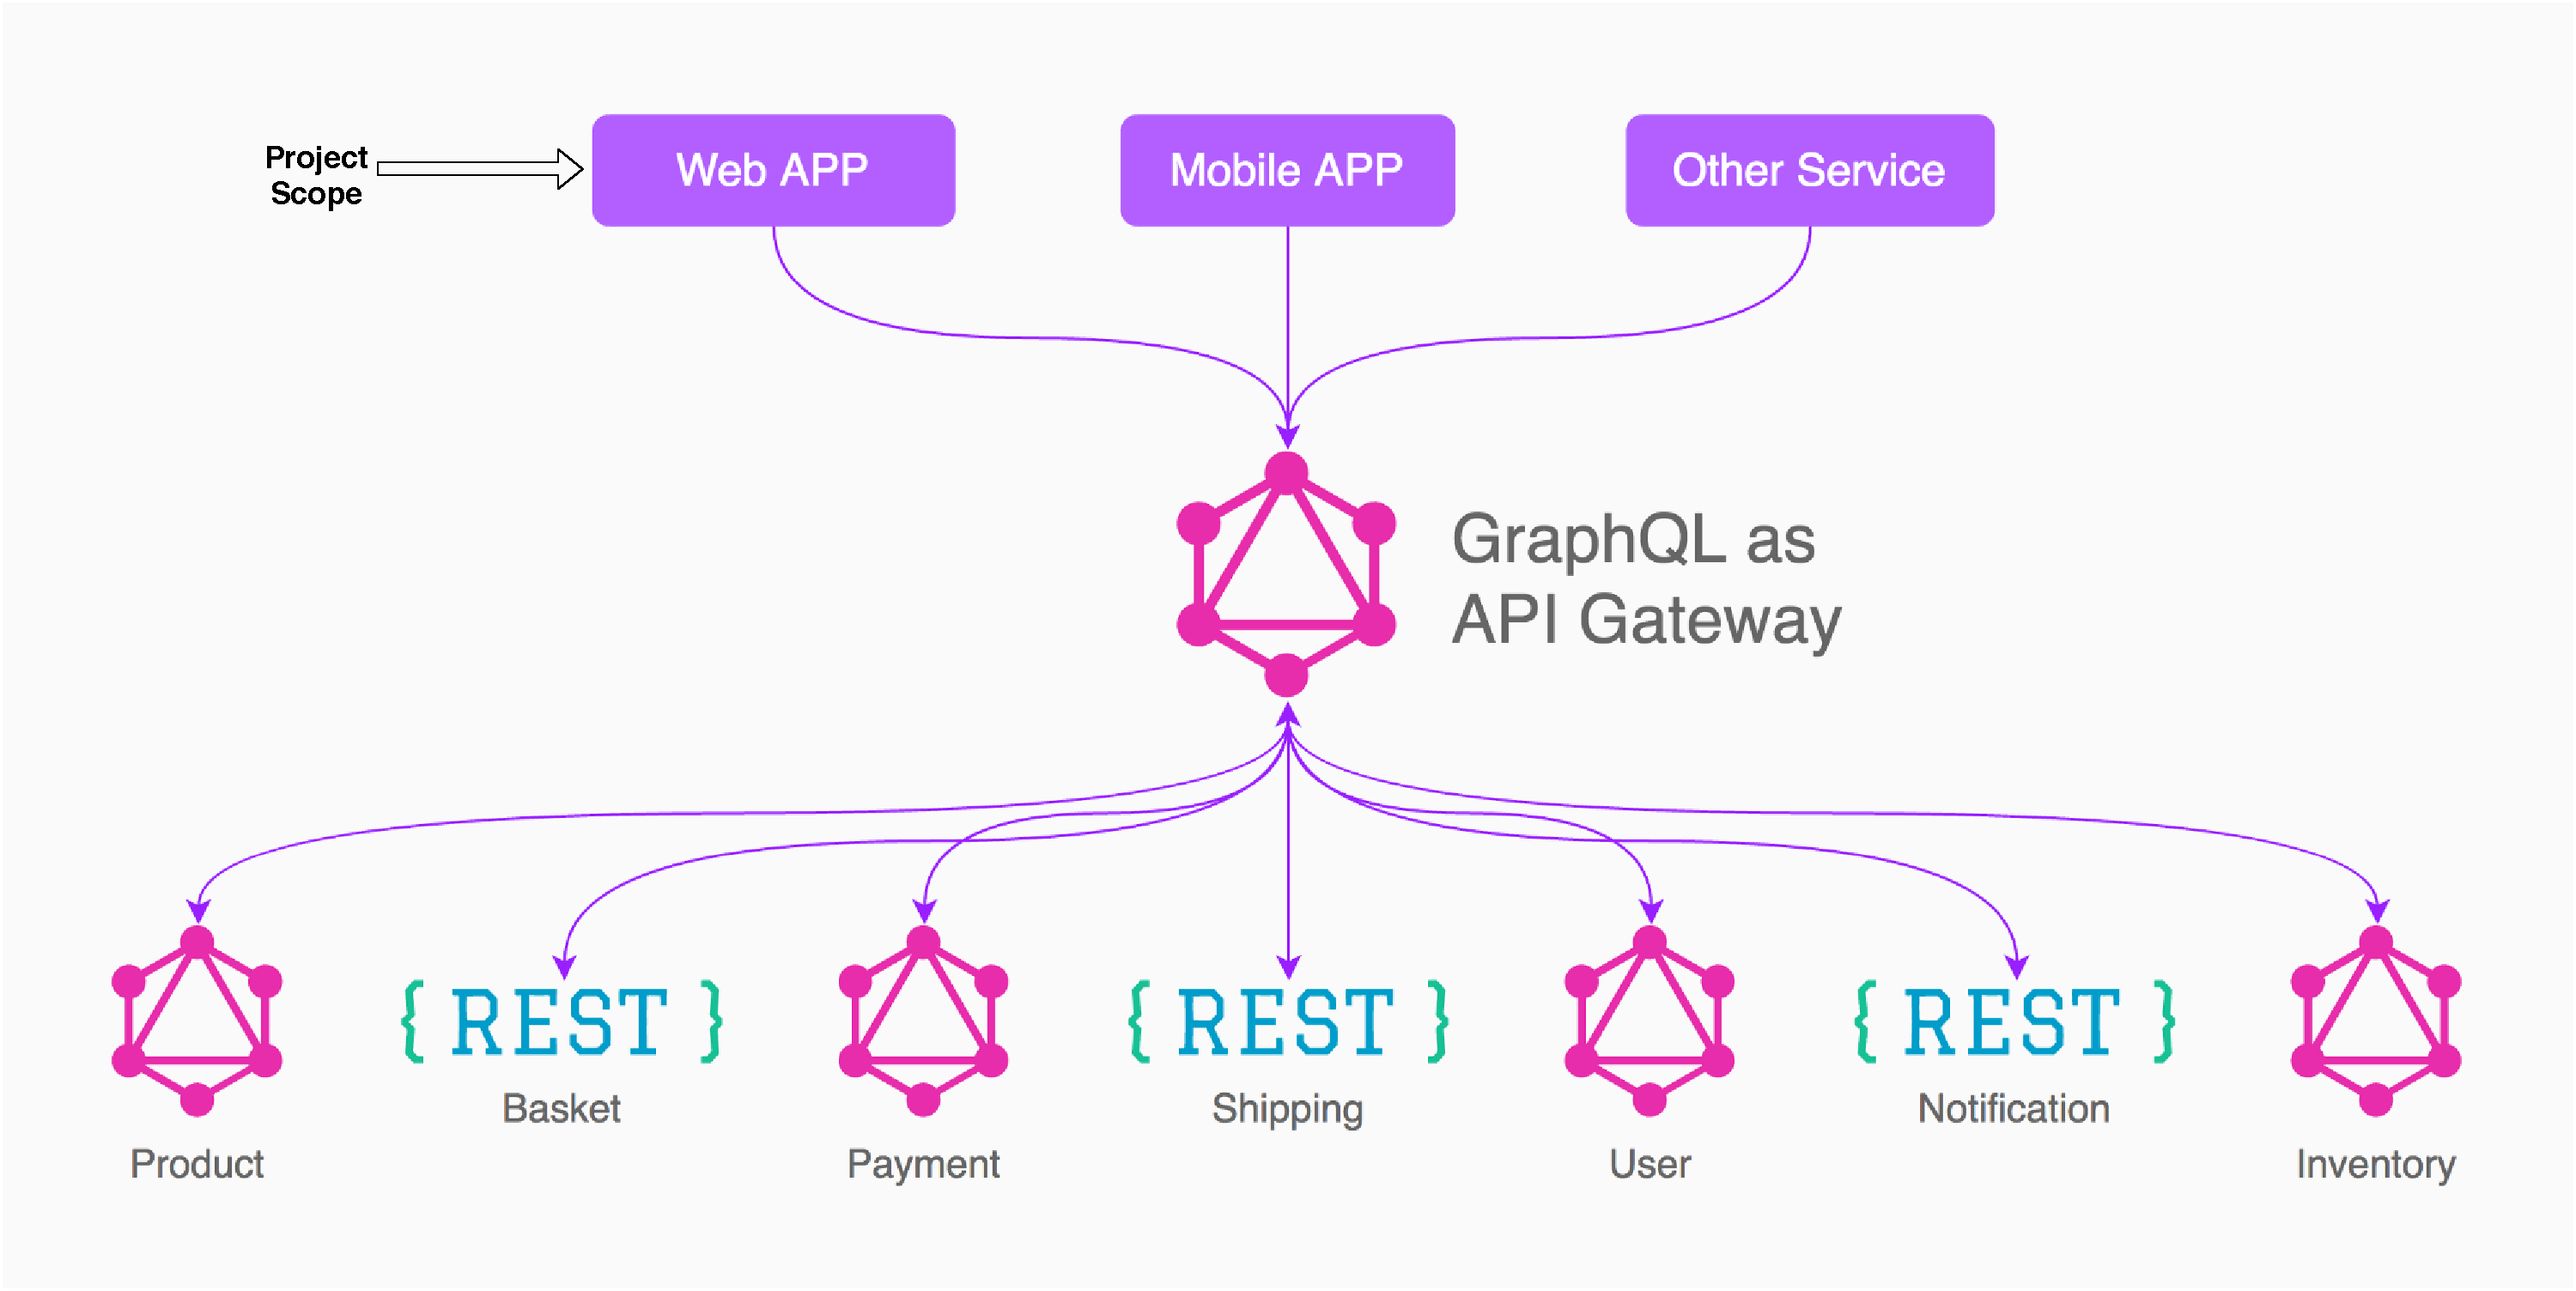
\includegraphics[width=15cm]{images/APIDiagram.pdf} 
\centering
\caption{API Diagram}
\label{api:diag}
\end{figure}

\subsection{Communication Interfaces}
Based on the project requirements and keeping the communication channels in mind, the chosen technology stack for the client-end is: TypeScript, React, and \href{https://github.com/apollographql/react-apollo}{React Apollo} (for interacting with the GraphQL API), and for the server-end is: Python, Django, and \href{https://github.com/graphql-python/graphene-django}{Graphene Django} (for creating the GraphQL API). \autoref{table:tech-server}, \autoref{table:tech-client}, and \autoref{table:tech-api} offer a detailed comparison between why these communication interfaces were picked over some of their major competitors.


\section{Use Cases}
The two main users of the system are customers and the admin. \autoref{usecases} summarizes their system use cases.
\begin{figure}[H]
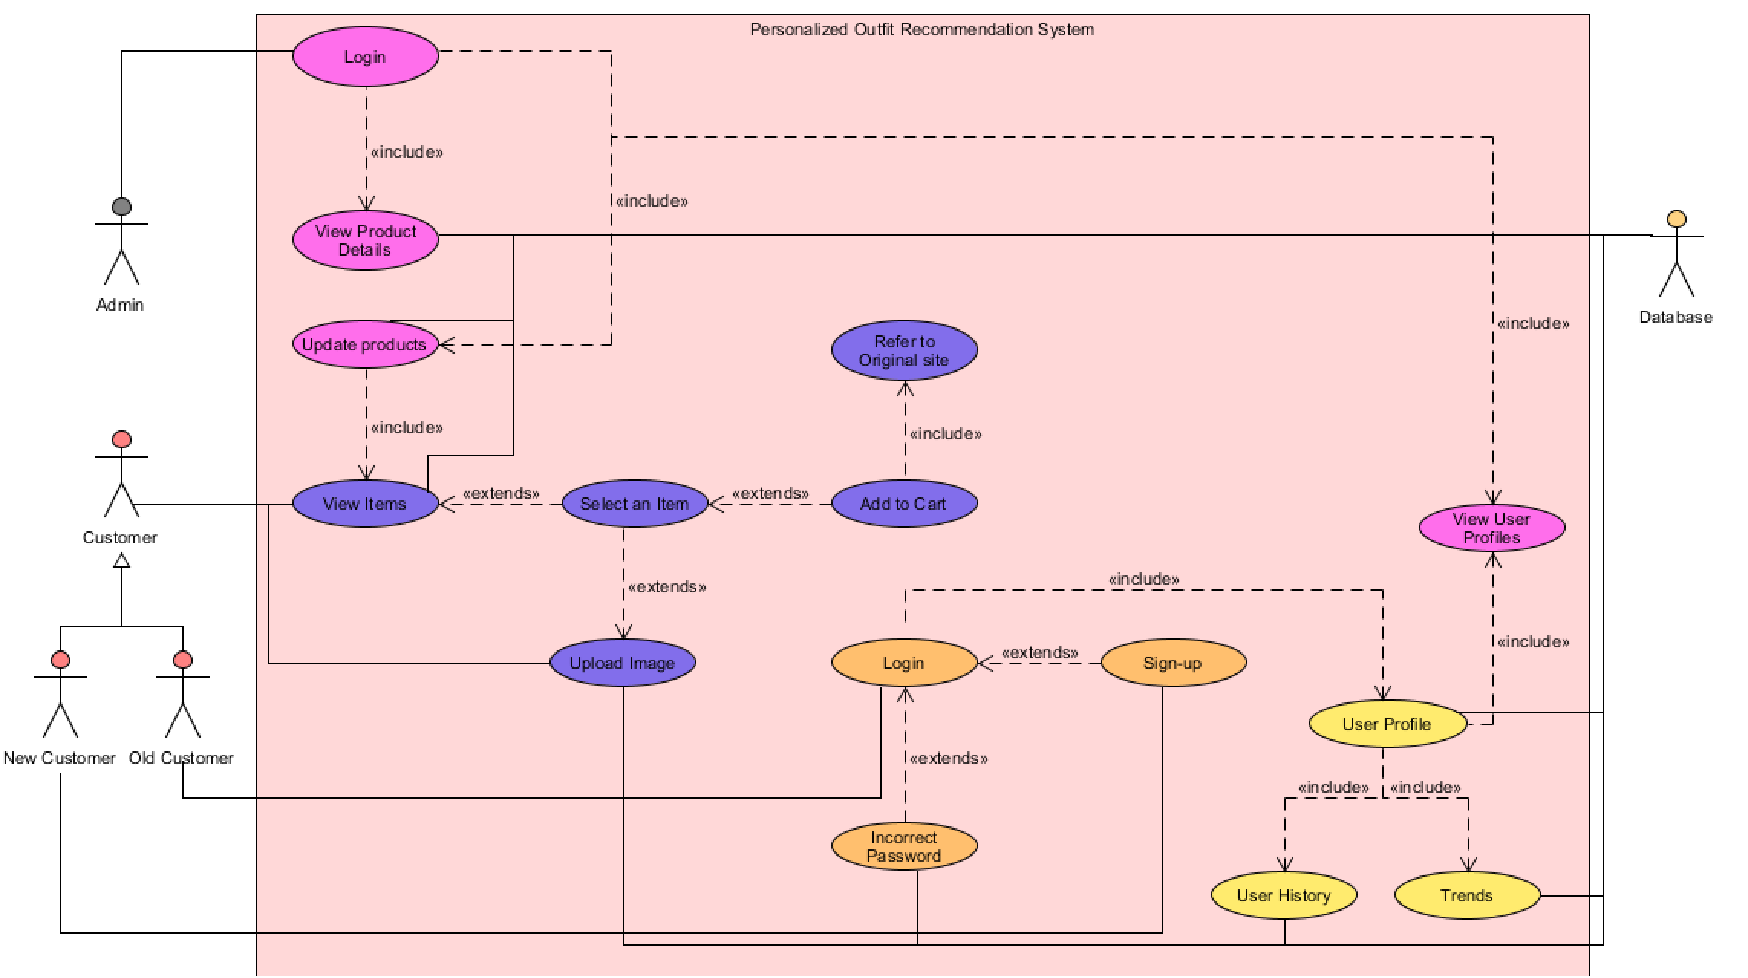
\includegraphics[width=15cm]{images/UseCaseDiag.pdf} 
\centering
\caption{Use-Case Diagram}
\label{usecases}
\end{figure}


\subsection{User Login}
\begin{center}
    \begin{tabular}{ @{}|p{7cm}||p{7cm}|  }
    \hline
    Use-Case Name: & Login  \\ \hline
    Use-Case ID: & PORS-01 \\ \hline
    Priority: & High \\ \hline
    Primary Business Actor: & System Admin \\ \hline
    Other Participating Actors: & Customer \\ \hline
    Description: & System admin needs to login in order to view customer, product details and update the stock. Whereas, the customer needs to login to view the referred sites and save his profile \\ \hline
    Pre-condition: & User has registered previously on the app and has valid email and password.  \\ \hline
    Trigger: & This use case is initiated when the admin wants to navigate the app or customer tries to view the referred site. \\ \hline
    Typical course of events: & \textbf{Actor Action:} \newline Actor enters valid username and password. \newline \textbf{System Action:} \newline Checks if the given username is registered in database and the given password is valid.
 \\ \hline
    Alternate courses: & If the credentials are invalid then an error message is displayed.  \\ \hline
    Conclusion: &  User successfully logs in using valid credentials.\\ \hline
    Post-condition: & User login is logged in the database. \\ \hline
    \end{tabular}
\end{center}

\subsection{View Product Details}
\begin{center}
    \begin{tabular}{ @{}|p{7cm}||p{7cm}|  }
    \hline
    Use-Case Name: & View Product Details  \\ \hline
    Use-Case ID: & PORS-02 \\ \hline
    Priority: & High \\ \hline
    Primary Business Actor: & System Admin \\ \hline
    Other Participating Actors: & Customer \\ \hline
    Description: & System Admin will view the product details to be able to update the stock. Whereas the customer will be able to see the product with details in order to select the items of their choice. \\ \hline
    Pre-condition: & Logged in as Admin or Customer.  \\ \hline
    Trigger: & This use case is triggered when the user clicks a product. \\ \hline
    Typical course of events: & Appropriate product details will be displayed to the user. \\ \hline
    Alternate courses: & None \\ \hline
    Conclusion: &  The user is able to see the product detail page.\\ \hline
    Post-condition: & User search is logged in the database.  \\ \hline
    \end{tabular}
\end{center}

\subsection{Update Stock}

\begin{center}
    \begin{tabular}{ @{}|p{7cm}||p{7cm}|  }
    \hline
    Use-Case Name: & Update Stock  \\ \hline
    Use-Case ID: & PORS-03 \\ \hline
    Priority: & High \\ \hline
    Primary Business Actor: & System Admin \\ \hline
    Other Participating Actors: & None \\ \hline
    Description: & System Admin will be able to update new stock and product details in case a product is sold out. \\ \hline
    Pre-condition: & Logged in as Admin.  \\ \hline
    Trigger: & This use case will be triggered when the system admin clicks update stock button. \\ \hline
    Typical course of events: & \textbf{System Action:} \newline System will check all the products and update the sold out and new products accordingly.
 \\ \hline
    Alternate courses: & None \\ \hline
    Conclusion: & The stock is successfully updated. \\ \hline
    Post-condition: & Customers are able to view the updated stock.\\ \hline
    \end{tabular}
\end{center}

\subsection{Upload an Image}

\begin{center}
    \begin{tabular}{ @{}|p{7cm}||p{7cm}|  }
    \hline
    Use-Case Name: & Upload an Image  \\ \hline
    Use-Case ID: & PORS-04 \\ \hline
    Priority: & High \\ \hline
    Primary Business Actor: & Customer \\ \hline
    Other Participating Actors: & None \\ \hline
    Description: & Application will allow customers to upload an image of their piece of clothing in order to find a similar or complementary items. \\ \hline
    Pre-condition: & None \\ \hline
    Trigger: & This use case will be triggered when the user will click upload image option. \\ \hline
    Typical course of events: & \textbf{System Action:} \newline System will check if the uploaded photo is of a piece of clothing
 \\ \hline
    Alternate courses: & If the uploaded image is not recognizable, a suitable error message is displayed. \\ \hline
    Conclusion: & Customer’s valid picture will be uploaded on the app. \\ \hline
    Post-condition: & Customer will be able to see the recommendation according to the uploaded picture. \\ \hline
    \end{tabular}
\end{center}

\subsection{Add to Cart}

\begin{center}
    \begin{tabular}{ @{}|p{7cm}||p{7cm}|  }
    \hline
    Use-Case Name: & Add to Cart  \\ \hline
    Use-Case ID: & PORS-05 \\ \hline
    Priority: & High \\ \hline
    Primary Business Actor: & Customer \\ \hline
    Other Participating Actors: & None \\ \hline
    Description: & Items selected by the customer will be added to the cart in order to proceed to the original referral site. \\ \hline
    Pre-condition: & None \\ \hline
    Trigger: & This use case will be triggered when the customer will select an item and click the option ‘add to cart’. \\ \hline
    Typical course of events: & System will check if the product is available to be added to the cart. \\ \hline
    Alternate courses: & None \\ \hline
    Conclusion: &  Selected item will be added to the customer’s cart.\\ \hline
    Post-condition: &  Valid referral link to the item is updated. \\ \hline
    \end{tabular}
\end{center}

\subsection{Refer to Original Sites}
\begin{center}
    \begin{tabular}{ @{}|p{7cm}||p{7cm}|  }
    \hline
    Use-Case Name: & Refer to Original Sites  \\ \hline
    Use-Case ID: & PORS-06 \\ \hline
    Priority: & Medium \\ \hline
    Primary Business Actor: & Customer \\ \hline
    Other Participating Actors: & None \\ \hline
    Description: & Once the customer has selected items of his choice, those will be added to the cart and then he would be redirected to the original product site.
 \\ \hline
    Pre-condition: & Items added to the cart \\ \hline
    Trigger: & This use case will be triggered when a customer clicks on ‘proceed to original site’ option, available in his cart. \\ \hline
    Typical course of events: & \textbf{System Action:} \newline System will direct the customer to the original sites of the items available in customer’s cart
 \\ \hline
    Alternate courses: & None\\ \hline
    Conclusion: &  Customer directed to the original sites of the items he has chosen.\\ \hline
    Post-condition: &  Reference point is logged in the dataset. \\ \hline
    \end{tabular}
\end{center}

\subsection{Sign-up}

\begin{center}
    \begin{tabular}{ @{}|p{7cm}||p{7cm}|  }
    \hline
    Use-Case Name: & Sign-up  \\ \hline
    Use-Case ID: & PORS-07 \\ \hline
    Priority: & High \\ \hline
    Primary Business Actor: & Admin \\ \hline
    Other Participating Actors: & Customer \\ \hline
    Description: & Admin and Customers will have to sign-up and register on the app in order to login and proceed. \\ \hline
    Pre-condition: & Valid information by the user. \\ \hline
    Trigger: & This use case will be triggered when a new user wants to register on the application. \\ \hline
    Typical course of events: & \textbf{Actor Action:} \newline Providing valid details.\newline \textbf{System Action:} \newline Checking if the details provided are available in the database.
 \\ \hline
    Alternate courses: & If the details provided are incomplete or already registered then appropriate error message must be displayed. \\ \hline
    Conclusion: &  User is able to sign-up successfully.\\ \hline
    Post-condition: & New user is added to the database. \\ \hline
    \end{tabular}
\end{center}

\subsection{Incorrect Password}
\begin{center}
    \begin{tabular}{ @{}|p{7cm}||p{7cm}|  }
    \hline
    Use-Case Name: & Incorrect Password \\ \hline
    Use-Case ID: & PORS-08\\ \hline
    Priority: & High \\ \hline
    Primary Business Actor: & Admin, Customer \\ \hline
    Other Participating Actors: &  None \\ \hline
    Description: & While logging-in on the app, the user must enter a valid email and password.\\ \hline
    Pre-condition: & Registered on the app. \\ \hline
    Trigger: &  This use case will be triggered when a user tried to login with incorrect password or username. \\ \hline
    Typical course of events: & \textbf{System Action:} \newline System checks if the given password or user-name is registered in the database.  \\ \hline
    Alternate courses: & System displays an error message about incorrect credentials. \\ \hline
    Conclusion: & User unable to login to the app. \\ \hline
    Post-condition: & Incorrect login attempt is logged in the database. \\ \hline
    \end{tabular}
\end{center}

\subsection{User Profile}
\begin{center}
    \begin{tabular}{ @{}|p{7cm}||p{7cm}|  }
    \hline
    Use-Case Name: & User Profile \\ \hline
    Use-Case ID: & PORS-09 \\ \hline
    Priority: & Medium \\ \hline
    Primary Business Actor: & Customer \\ \hline
    Other Participating Actors: & System Admin \\ \hline
    Description: & All registered users will have user profiles displaying their details, purchase history and uploaded image history. \\ \hline
    Pre-condition: & User must be logged in. \\ \hline
    Trigger: & This use case will be triggered when the admin wants to look at a particular user’s profile or the customer himself clicks at his profile. \\ \hline
    Typical course of events: &  System will display the updated user profile to the user. \\ \hline
    Alternate courses: & None \\ \hline
    Conclusion: &  User profile displayed.\\ \hline
    Post-condition: &  None\\ \hline
    \end{tabular}
\end{center}

\subsection{User History}
\begin{center}
    \begin{tabular}{ @{}|p{7cm}||p{7cm}|  }
    \hline
    Use-Case Name: & User History \\ \hline
    Use-Case ID: & PORS-10\\ \hline
    Priority: & Medium \\ \hline
    Primary Business Actor: & Customer \\ \hline
    Other Participating Actors: & System Admin \\ \hline
    Description: & All registered users will have their user history comprising of purchase history and uploaded image history. \\ \hline
    Pre-condition: & 1.	User is registered in the database. \newline 2. User has either purchased or uploaded an image before.
 \\ \hline
    Trigger: & This use case will be triggered when a user purchases an item or uploads any image. \\ \hline
    Typical course of events: &  System will update the user history when the user will purchase or upload an item.\\ \hline
    Alternate courses: & None\\ \hline
    Conclusion: & User history is updated at every purchase or upload, given that the user is logged in.\\ \hline
    Post-condition: &  None\\ \hline
    \end{tabular}
\end{center}

\subsection{View Trends}
\begin{center}
    \begin{tabular}{ @{}|p{7cm}||p{7cm}|  }
    \hline
    Use-Case Name: & View Trends \\ \hline
    Use-Case ID: & PORS-11 \\ \hline
    Priority: & Medium \\ \hline
    Primary Business Actor: & Customer \\ \hline
    Other Participating Actors: & None \\ \hline
    Description: & Different statistics will be displayed indicating the sales or ratings of each brand in last 30 days.  \\ \hline
    Pre-condition: &  users have either purchased or rated an item from any brand.\\ \hline
    Trigger: &  This use case will be triggered when the user clicks trend option. \\ \hline
    Typical course of events: & System will update the trend at each purchase or rating by the user. \\ \hline
    Alternate courses: & None\\ \hline
    Conclusion: &  User is able to see the most updated trends. \\ \hline
    Post-condition: &  Catalog matrix is updated in the database.\\ \hline
    \end{tabular}
\end{center}

\section{Datasets}
This section describes the specific dataset which will be used to build our system. An appropriate snapshot of the dataset is also included in . Futher details, whenever needed, will be presented in the appendix.

For purposes of the image classification pipeline for our recommendation engine, we have selected DeepFashion \cite{DeepFashion} as our preliminary dataset. The dataset consists over 800,000 diverse fashion images ranging from well-posed shop images to unconstrained consumer photos. What makes this dataset suitable towards our system is the fact that it is annotated with rich information of clothing items. Each image in this dataset is labelled with 50 categories, 1,000 descriptive attributes, bounding box and clothing landmarks, and this would kick-start the training of our classifier. A category-wise subset of the dataset is depicted in \autoref{dataset:DeepFashion}. 

It is important to clarify here that the DeepFashion dataset consists of product images from western stores and outlets, so the classifier would not generalize efficiently to products in the local eastern domain, which is a  requirement of our system. Moreover, there are limitations in the amount of products and datasets we can scrape from eastern fashion stores such as J., Export Leftovers, Zellbury, Daraz, etc. If we were to use these as the only data for training our classifier, the model would indubitably suffer from underfitting. In order to maintain a good fit, we will use the concept of Transfer Learning to re-train the classifier trained on DeepFashion on our local scraped dataset from the aforementioned local fashion stores.

\begin{figure}[H]
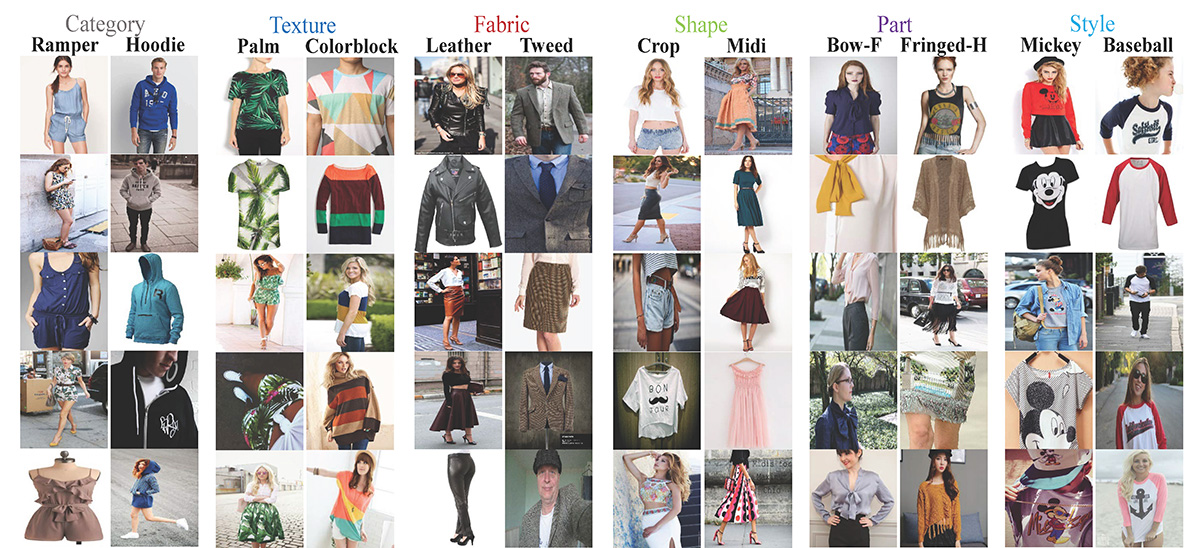
\includegraphics[width=15cm]{images/DeepFashion.pdf} 
\centering
\caption{The DeepFashion Dataset}
\label{dataset:DeepFashion}
\end{figure}

\section{System Diagram}
\label{srs:sysdiag}
\autoref{sysdiag:module} gives an overview of different modules of our system.
\begin{figure}[H]
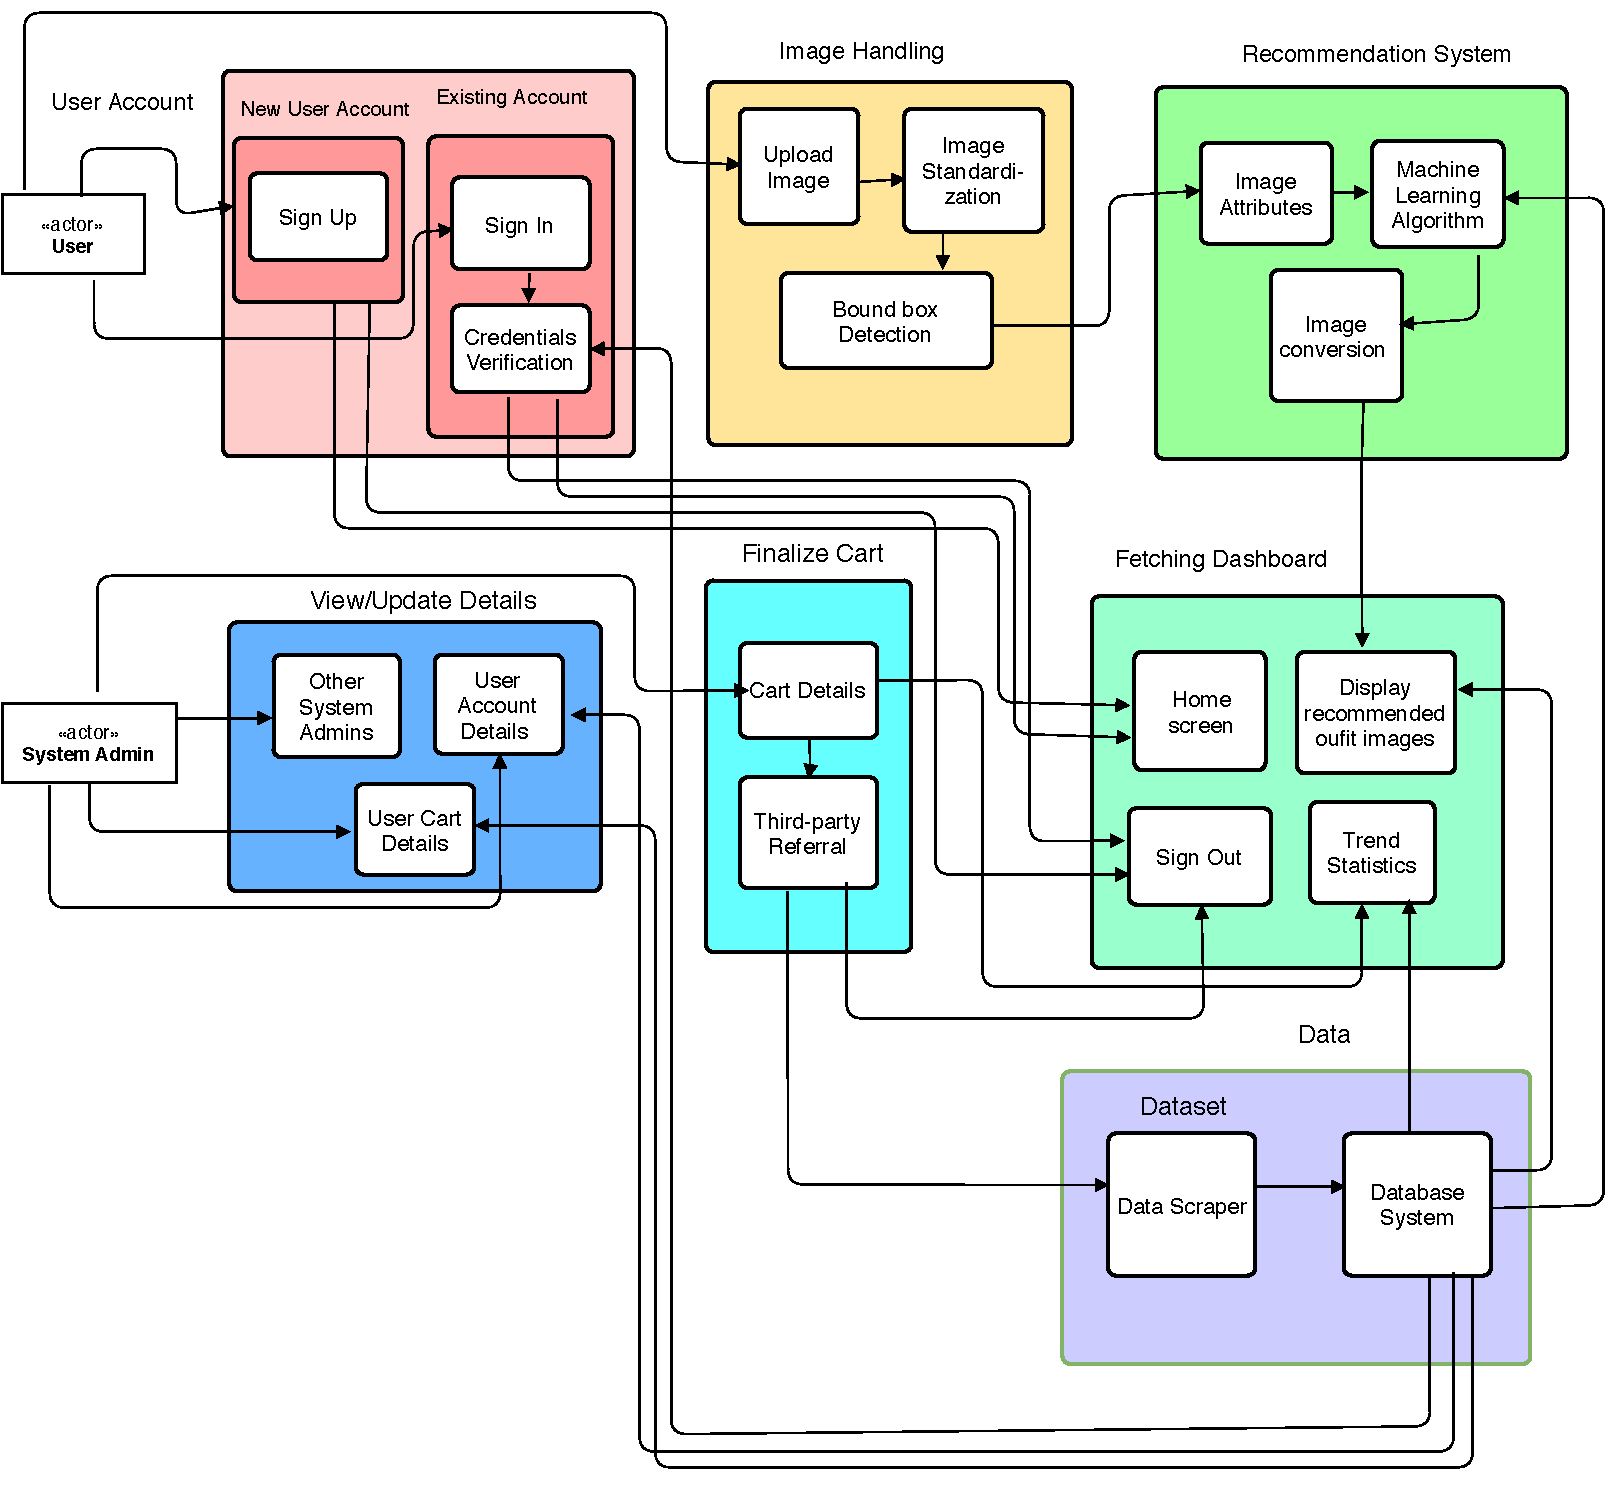
\includegraphics[width=15cm]{images/systemDiagramModule.pdf} 
\centering
\caption{Module-wise System Diagram}
\label{sysdiag:module}
\end{figure}
\autoref{sysdiag:tech} gives an overview of the chosen architecture of our system.
\begin{figure}[H]
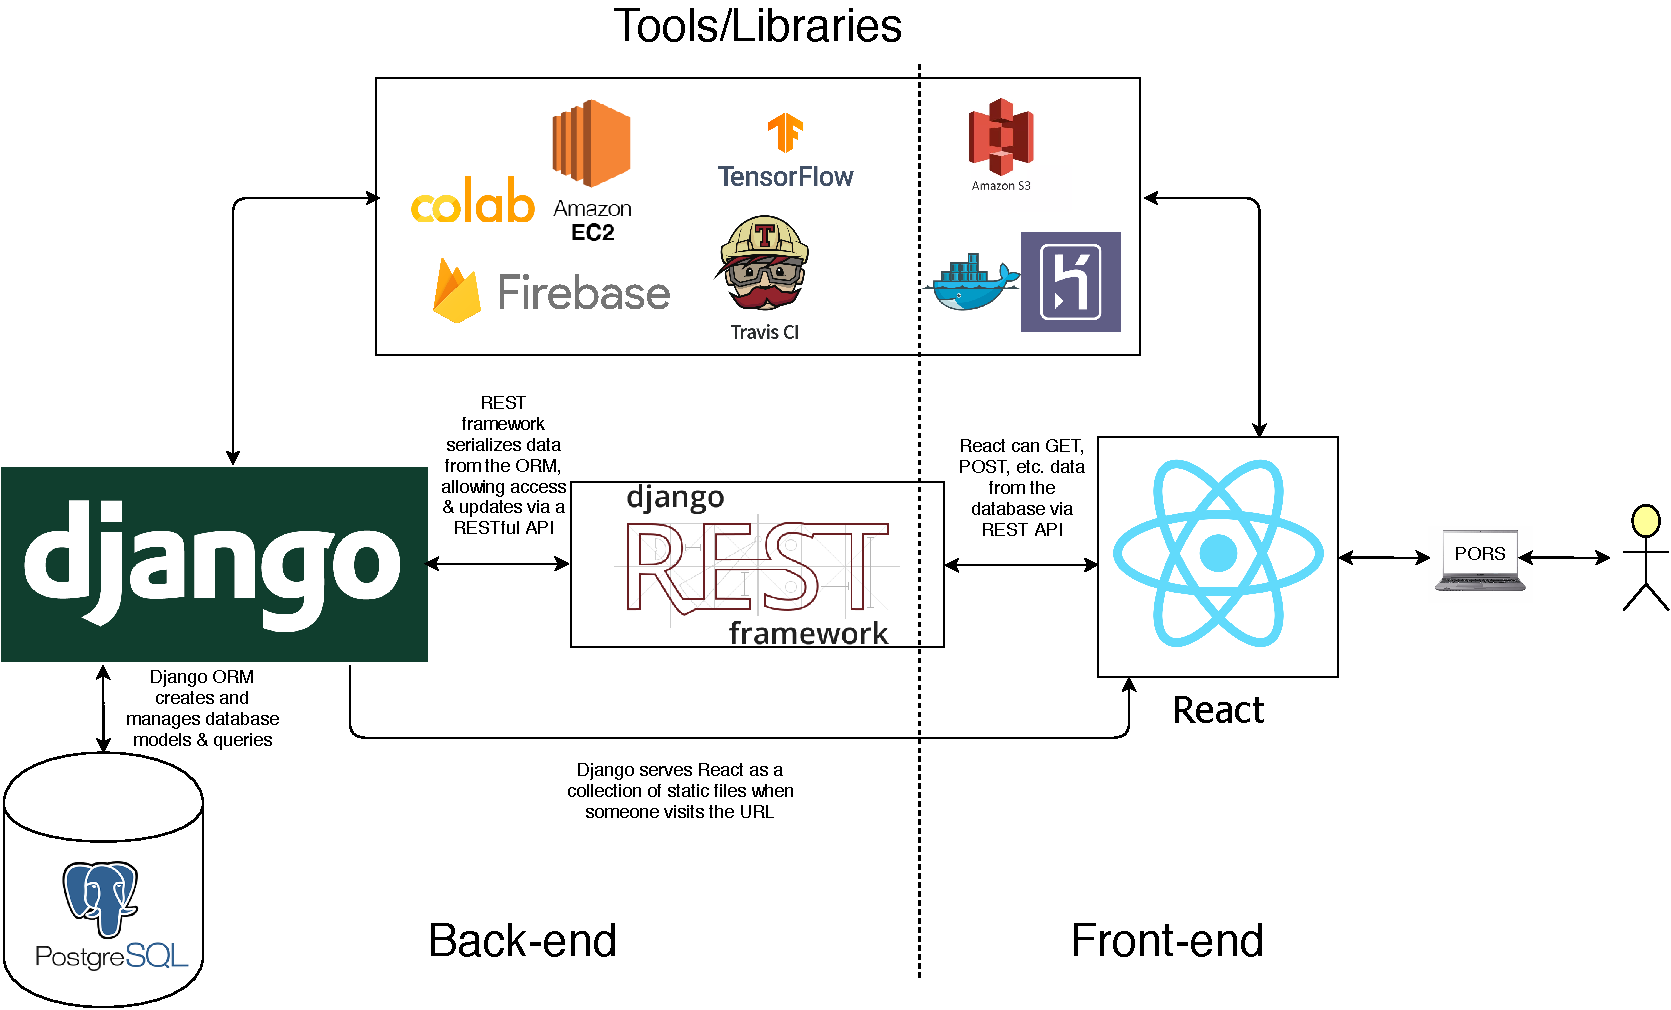
\includegraphics[width=15cm]{images/systemDiagramTech.pdf} 
\centering
\caption{Technology-wise System Diagram}
\label{sysdiag:tech}
\end{figure}

\section{Data Flow Diagram}
Rudimentary data flow diagrams for the system have also been constructed, given below in \autoref{dfd:context} and \autoref{dfd:zero}:

\begin{figure}[H]
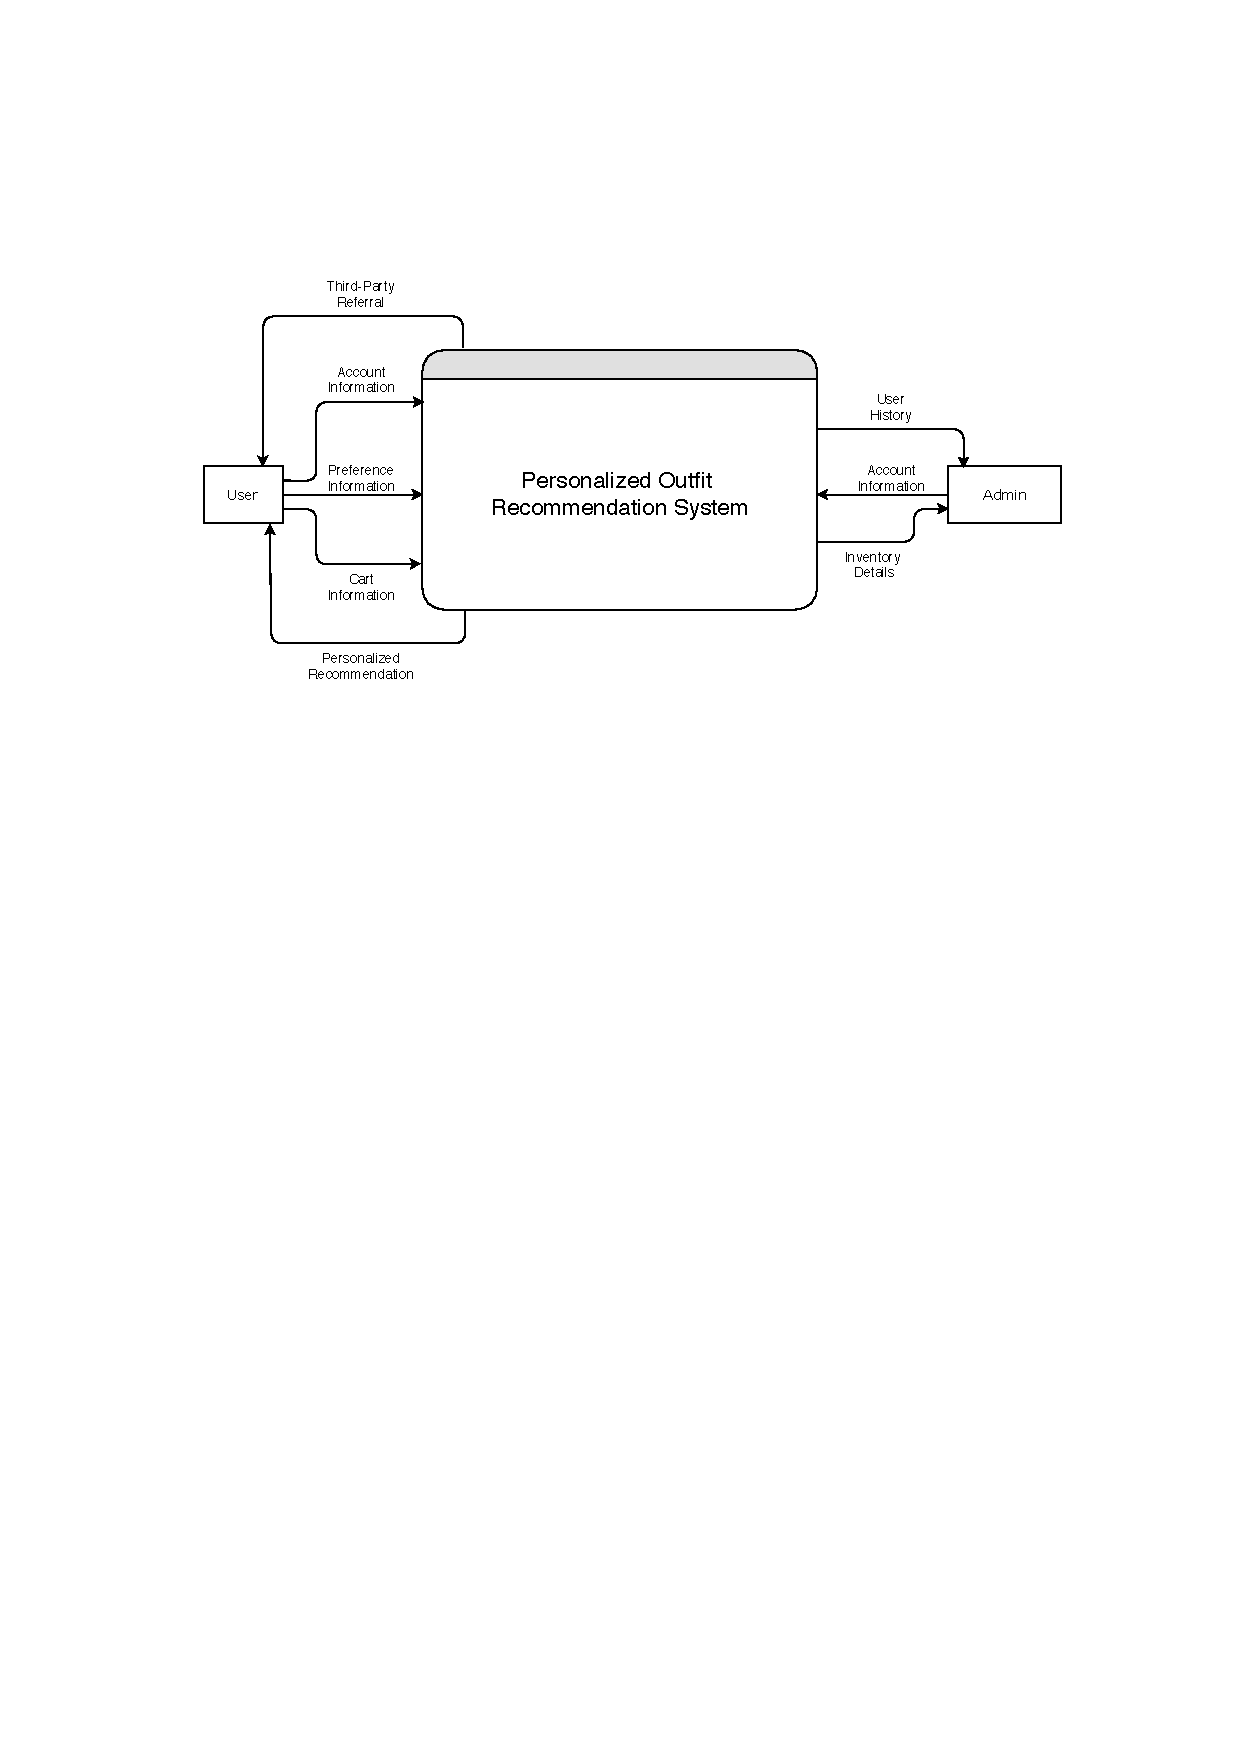
\includegraphics[width=15cm]{images/dfdContext.pdf} 
\centering
\caption{Context Level DFD}
\label{dfd:context}
\end{figure}

\begin{figure}[H]
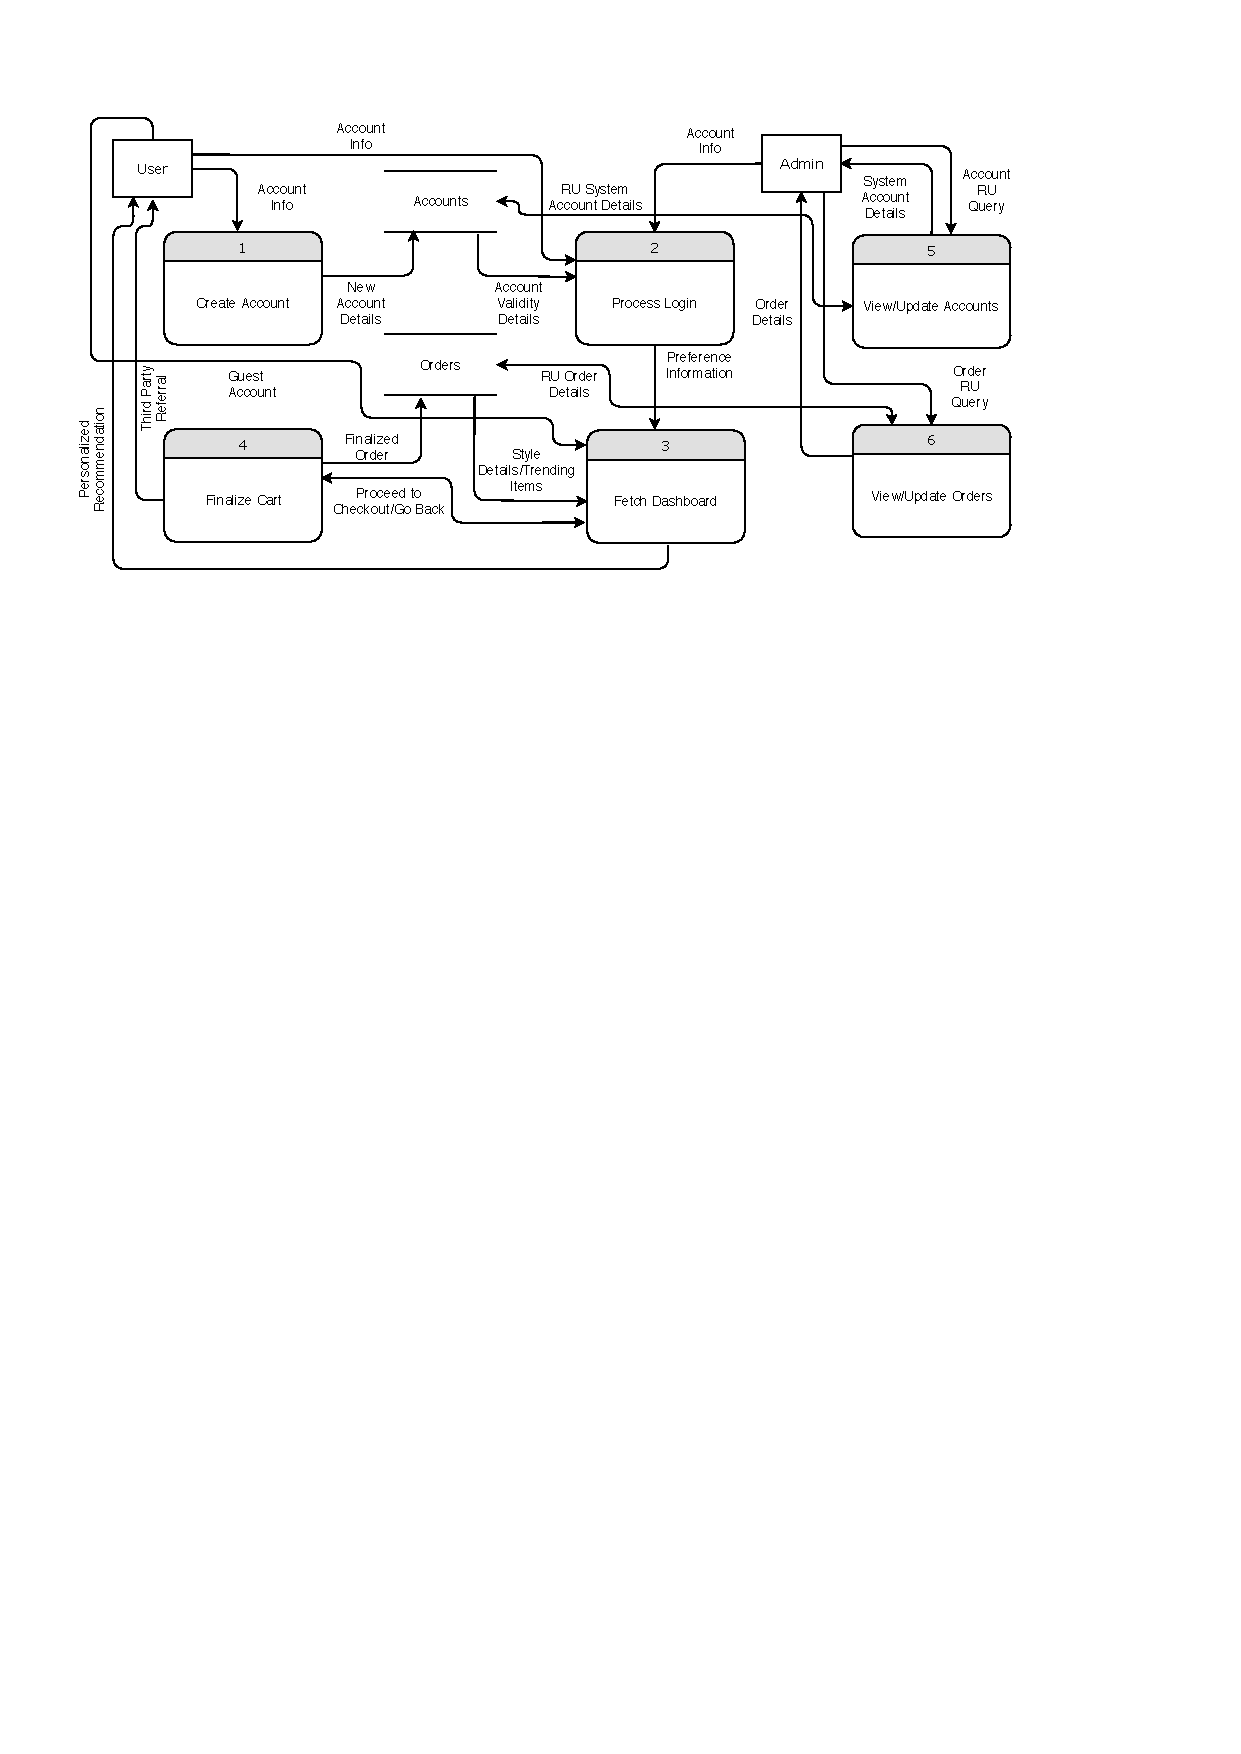
\includegraphics[width=15cm]{images/dfd0.pdf} 
\centering
\caption{0-Level DFD}
\label{dfd:zero}
\end{figure}

\section{Association Matrices}
Association matrices for the system are depicted in \autoref{crud:dToL}, \autoref{crud:dToP}, and \autoref{crud:pToL} ahead.  
\begin{table}
\centering
\begin{tabular}{ |c|c|c|c| } 
\hline
 & User & System Admin \\
\hline
\textbf{User} & Individual & All \\ \hline
User ID & R & CRUD \\ 
Name & RU & CRUD \\ 
Email ID & CRU & RD \\
Password & RU & RD \\
\hline
\textbf{Sign in/Sign up/ Sign out} & Individual & All \\ \hline
Account ID & R	& RD \\ 
Date &	R	& RD \\
\hline
\textbf{Verify Credentials} &	Individual	& All \\ \hline
Account Valid &	R &	CRUD \\
Logged In &	R &	CRUD \\
Date &	R &	CRUD \\
\hline
\textbf{Fetch Dashboard} &	Individual &	All \\ \hline
Page ID	& R	& CRUD \\
Image Details &	R &	CRUD\\ \hline
\textbf{Finalize Cart} &	Individual	& All \\ \hline
Cart ID	& R & CRUD \\
Date &	R &	CRUD \\
Item No. &	RU & CRUD \\
Third-party Referral &	R & CRUD \\ \hline
\textbf{Recommendation Details}	& Individual &	All \\ \hline
Recommendation ID &	R &	CRUD \\
User ID	& R & CRUD \\
Date &	R & CRUD \\ \hline
\textbf{Image} &	Individual	& All \\ \hline
Image ID &	R	& CRUD \\
Category & R & CRUD \\
Image Attribute	& R &	CRUD \\
Recommendation ID &	R &	CRUD \\ \hline

\hline
\end{tabular}
\caption{CRUD: Data to Location Matrix}
\label{crud:dToL}
\end{table}
\begin{table}
\centering
\begin{tabular}{ |c|c|c|c|c|c|} 
\hline
 & Account  & Credentials	& Dashboard & Cart & Image  \\
\hline
\textbf{User} &  &  &  &  & 5  \\ \hline
User ID	& R & R & R	& R &	R \\
Name &	CRU	& RU & & & \\	
Email &	CRU & R	& &	& R \\
Password &	CRU & R	& & & \\ \hline
\textbf{Sign in/up/out} & & & & & \\ \hline
Account ID	& R	& R & & & \\
Date &	R &	R & & & \\ \hline
\textbf{Verify Credentials} & & & & &\\ \hline		
Account Valid & & RU &	R &  & \\		
Logged In & & RU & R & & \\		
Date &	& R & R & & \\ \hline
\textbf{Fetch Dashboard} & & & & & \\ \hline		
Page ID	&	&	& R	& R & \\ 	
Image Details & & &	RUD	& RU & \\ \hline
\textbf{Finalize Cart} & & & & & \\ \hline		
Cart ID	&	& 	& R	& R & \\	
Date &	&	&	R &	RUD	& \\
Item No. &	&	&	R	& RUD & \\	
Third-party Referral &	&	&	R	& RUD & \\ \hline	
\textbf{Recommendation Details} & & & & & \\ \hline
Recommendation ID & & &	R	& RU & \\	
User ID	&	&	& R	& RUD & \\	
Date &	&	& R	& RUD & \\ \hline
\textbf{Image} & & & & & \\ \hline	
Image ID & & &	R & R & R \\ 
Category & & & RUD	& RUD & R \\
Image Attribute & & & RUD	& &	R \\
Recommendation ID & & &	R & R & R \\ \hline
\end{tabular}
\caption{CRUD: Data to Process Matrix}
\label{crud:dToP}
\end{table}

\begin{table}
\centering
\begin{tabular}{ |c|c|c| } 
\hline
 & User & System Admin \\
\hline
Process Account & * &  \\ \hline
Process Verify Credentials & & * \\ \hline
Process Dashboard &	 &	* \\ \hline
Process Cart &	*	&  \\ \hline
Process Image Handling &  & * \\ \hline
\end{tabular}
\caption{CRUD: Process to Location Matrix}
\label{crud:pToL}
\end{table}

\chapter{Software Design Specification (SDS)}
\label{chap:sds}

This chapter provides important artifacts related to design of our project.

% Your report will contain ONE of the following 2 sections.

\section{Data Design}

This section presents the structure of our database that caters to persistent data storage in our project. The structure is shown as a normalized data model for relational databases. It clearly shows entities, attributes, relationships with their cardinalities, and primary and foreign keys. We have used DB designer to build our data model.


\begin{figure}[H]
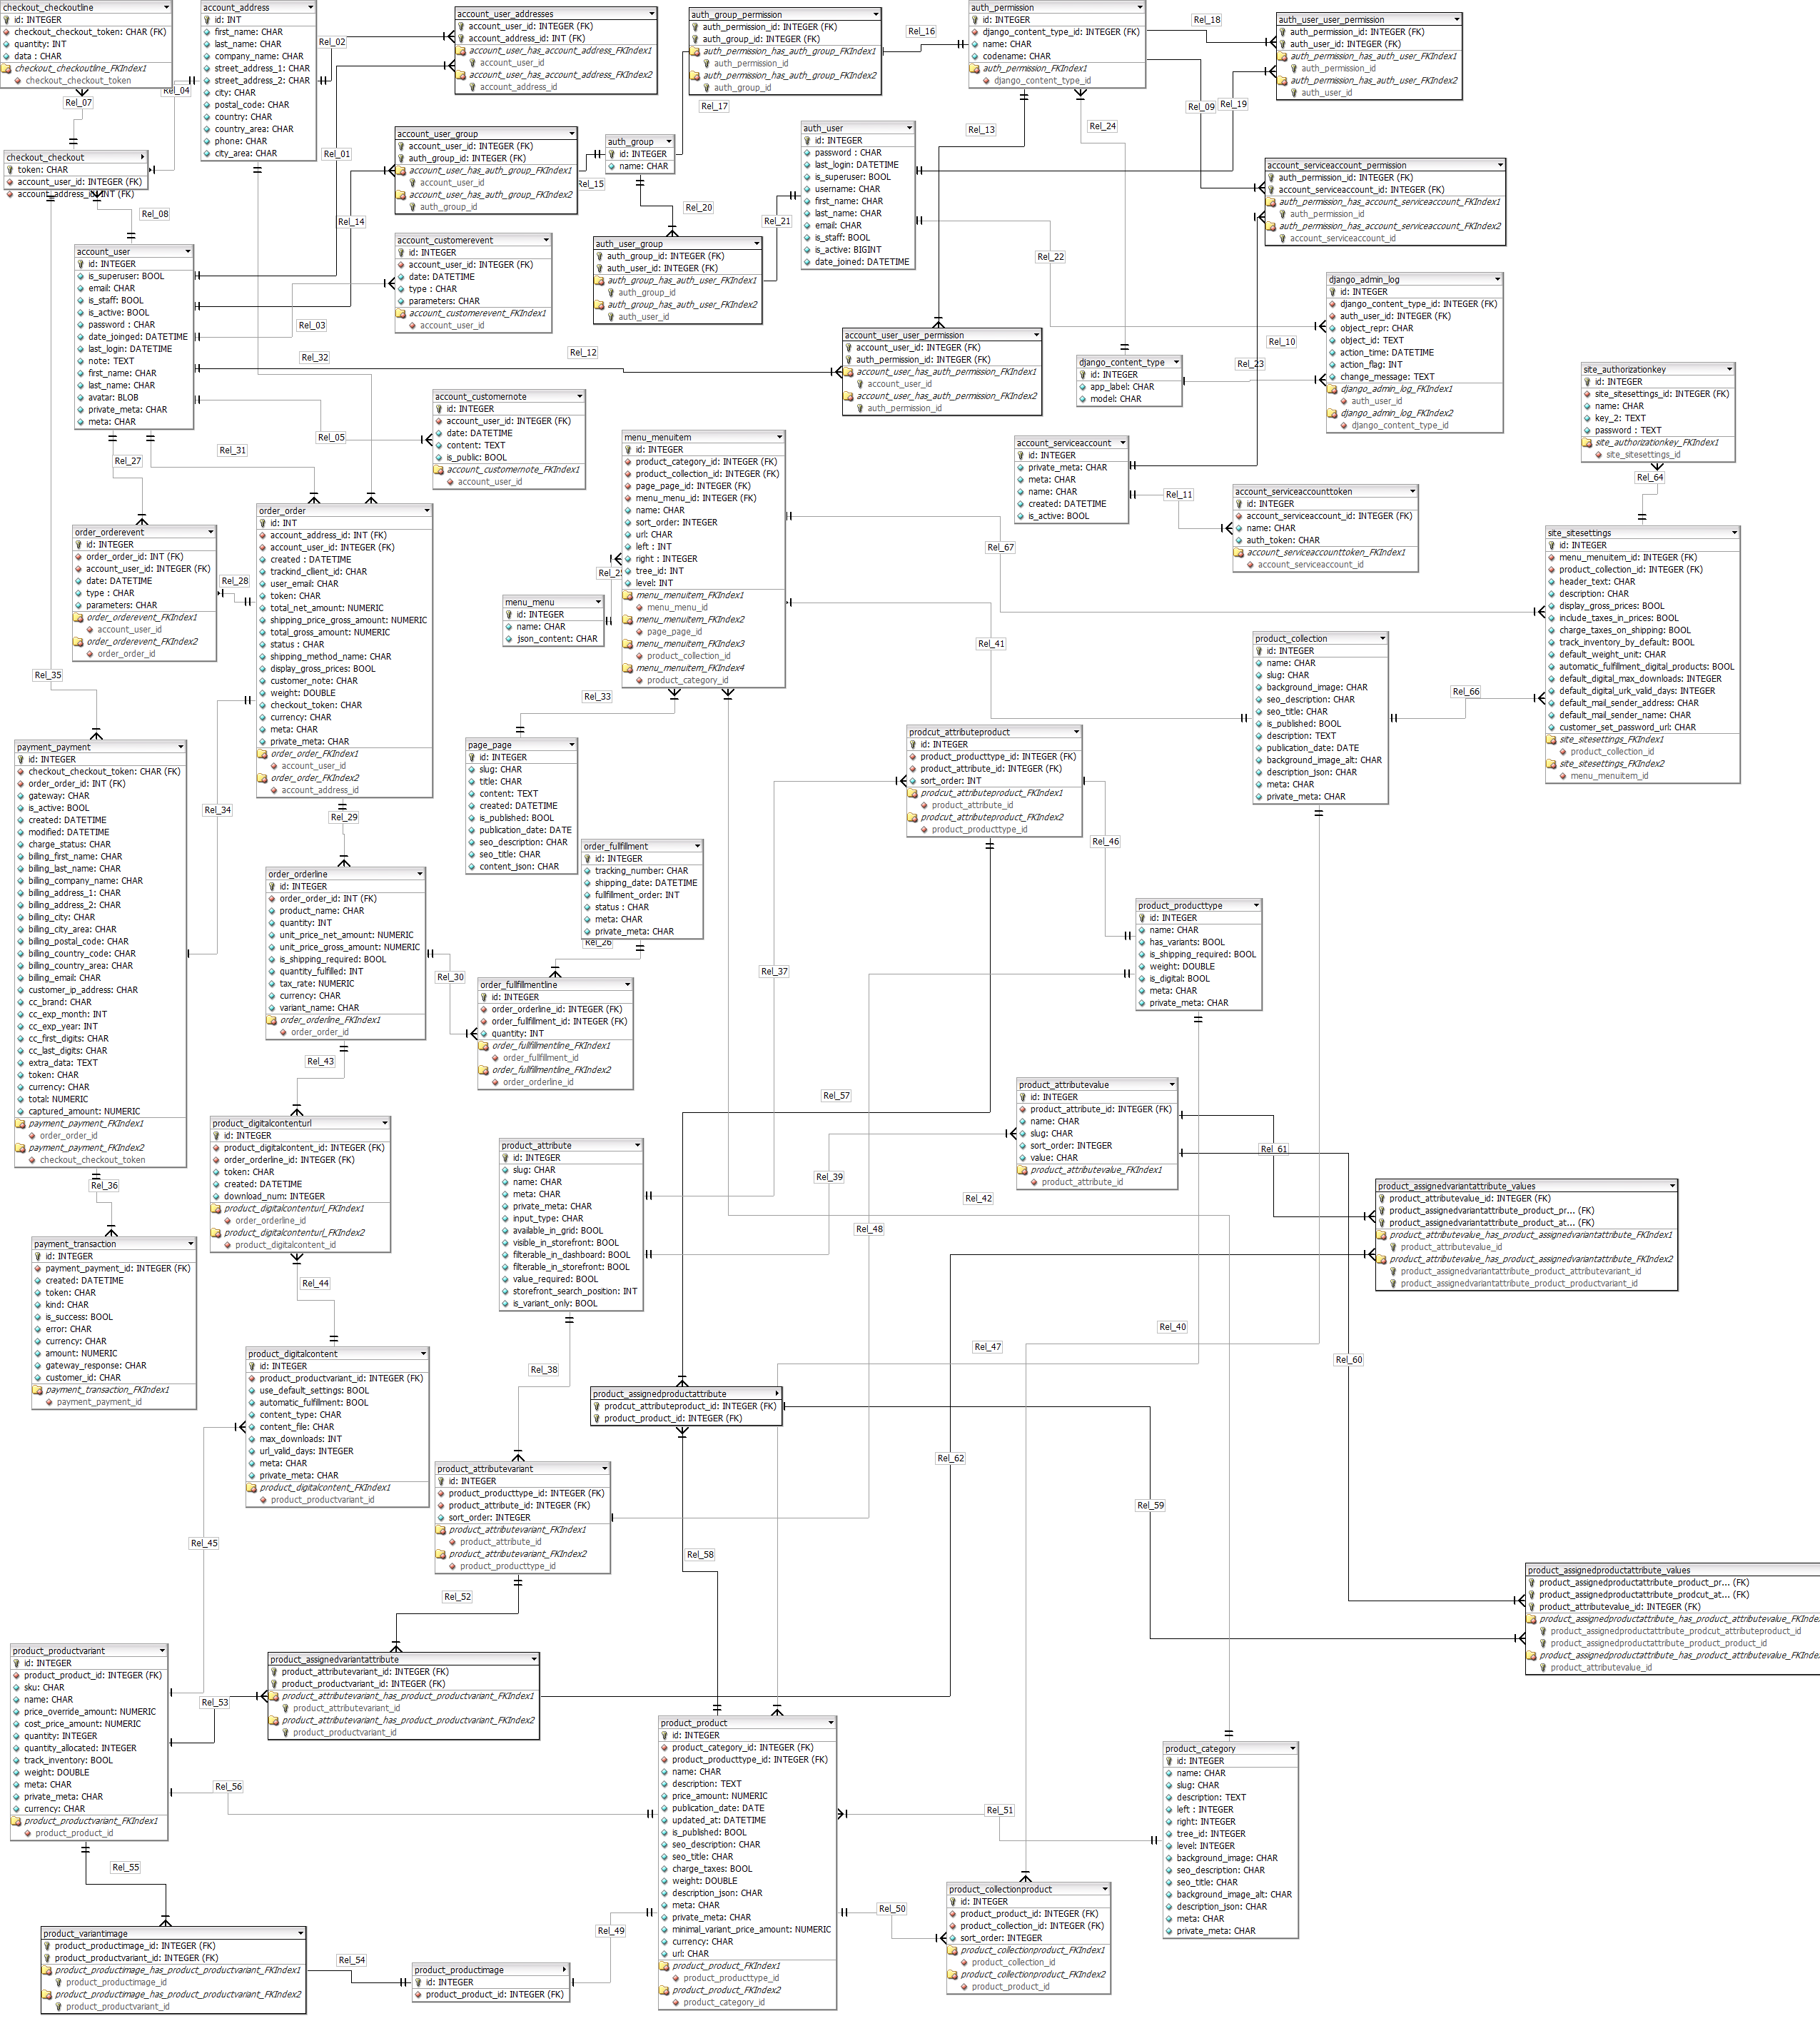
\includegraphics[width=15cm, height = 18cm, keepaspectratio]{images/PORS_ERD.png} 
\centering
\caption{Entity Relationship Diagram}
\label{erd}
\end{figure}
 
%\section{Technical Details}
%
%Our project does not have persistent data so we have no ERD. Instead we exaplin here the technical details of the algortihsm we use. These include the inputs and the outputs, how and where these algorothms fit in our tool chain, the techniques used in these algorithms, etc.

\section{State Diagram}

\begin{figure}[H]
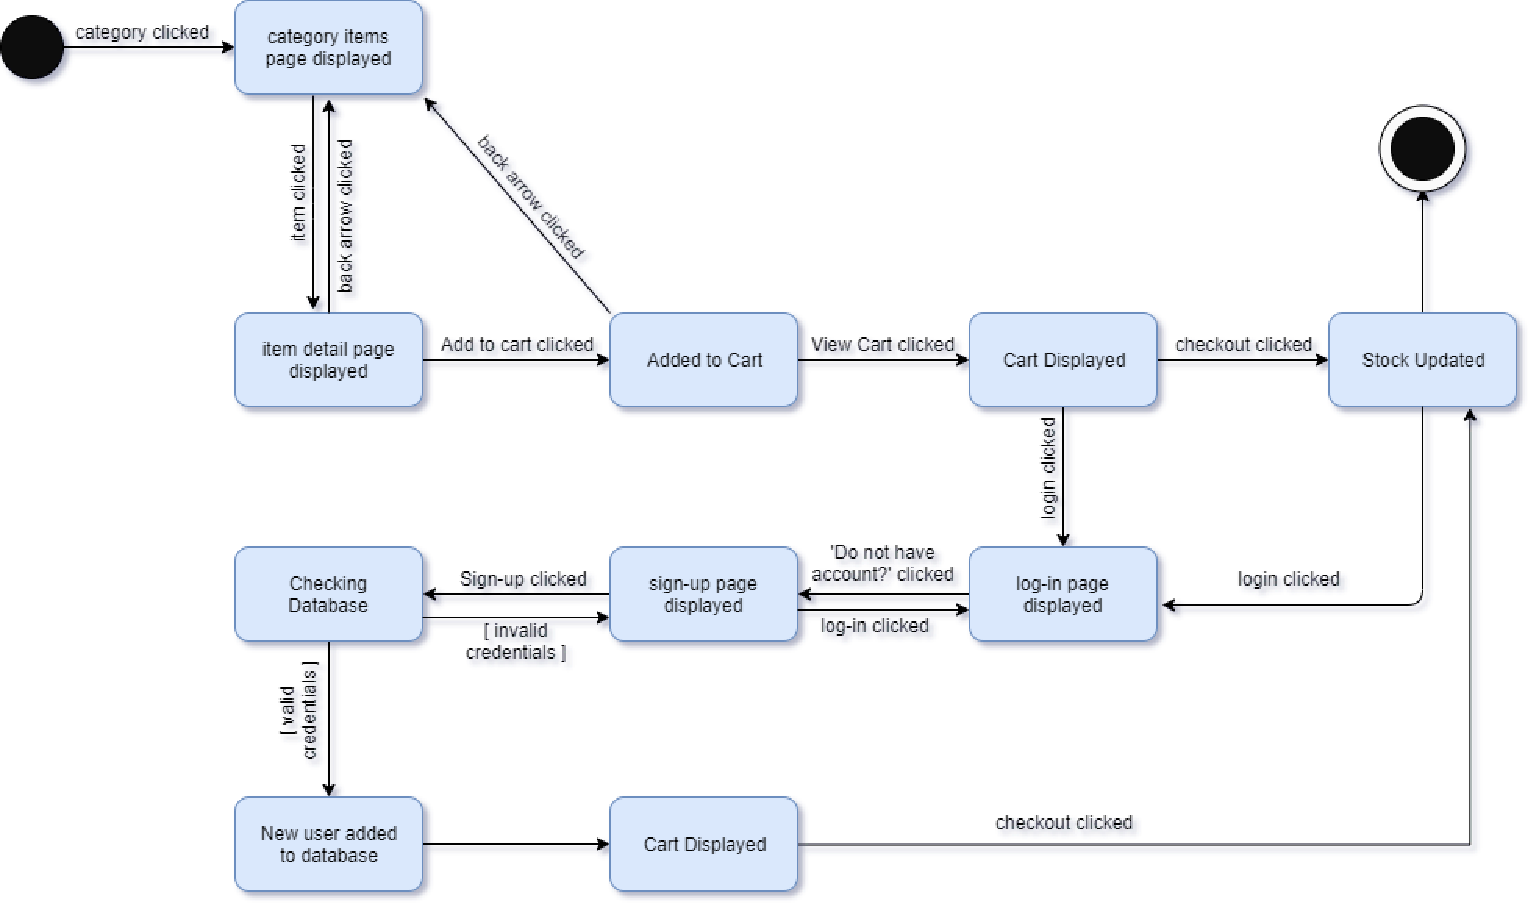
\includegraphics[width=10cm]{images/StateDiag1.pdf} 
\centering
\caption{State Diagram 1}
\label{state: one}
\end{figure}

\begin{figure}[H]
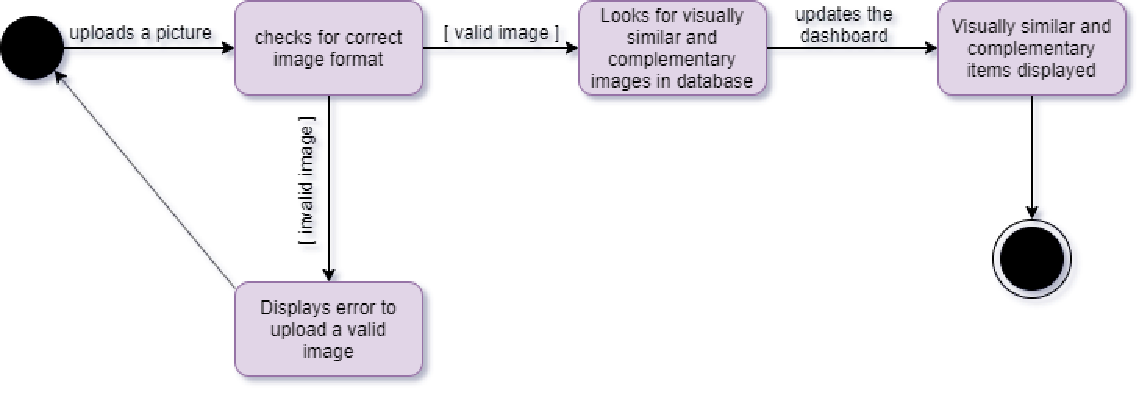
\includegraphics[width=10cm]{images/StateDiag2.pdf} 
\centering
\caption{State Diagram 2}
\label{state: two}
\end{figure}

\section{Sequence Diagram}
\begin{figure}[H]
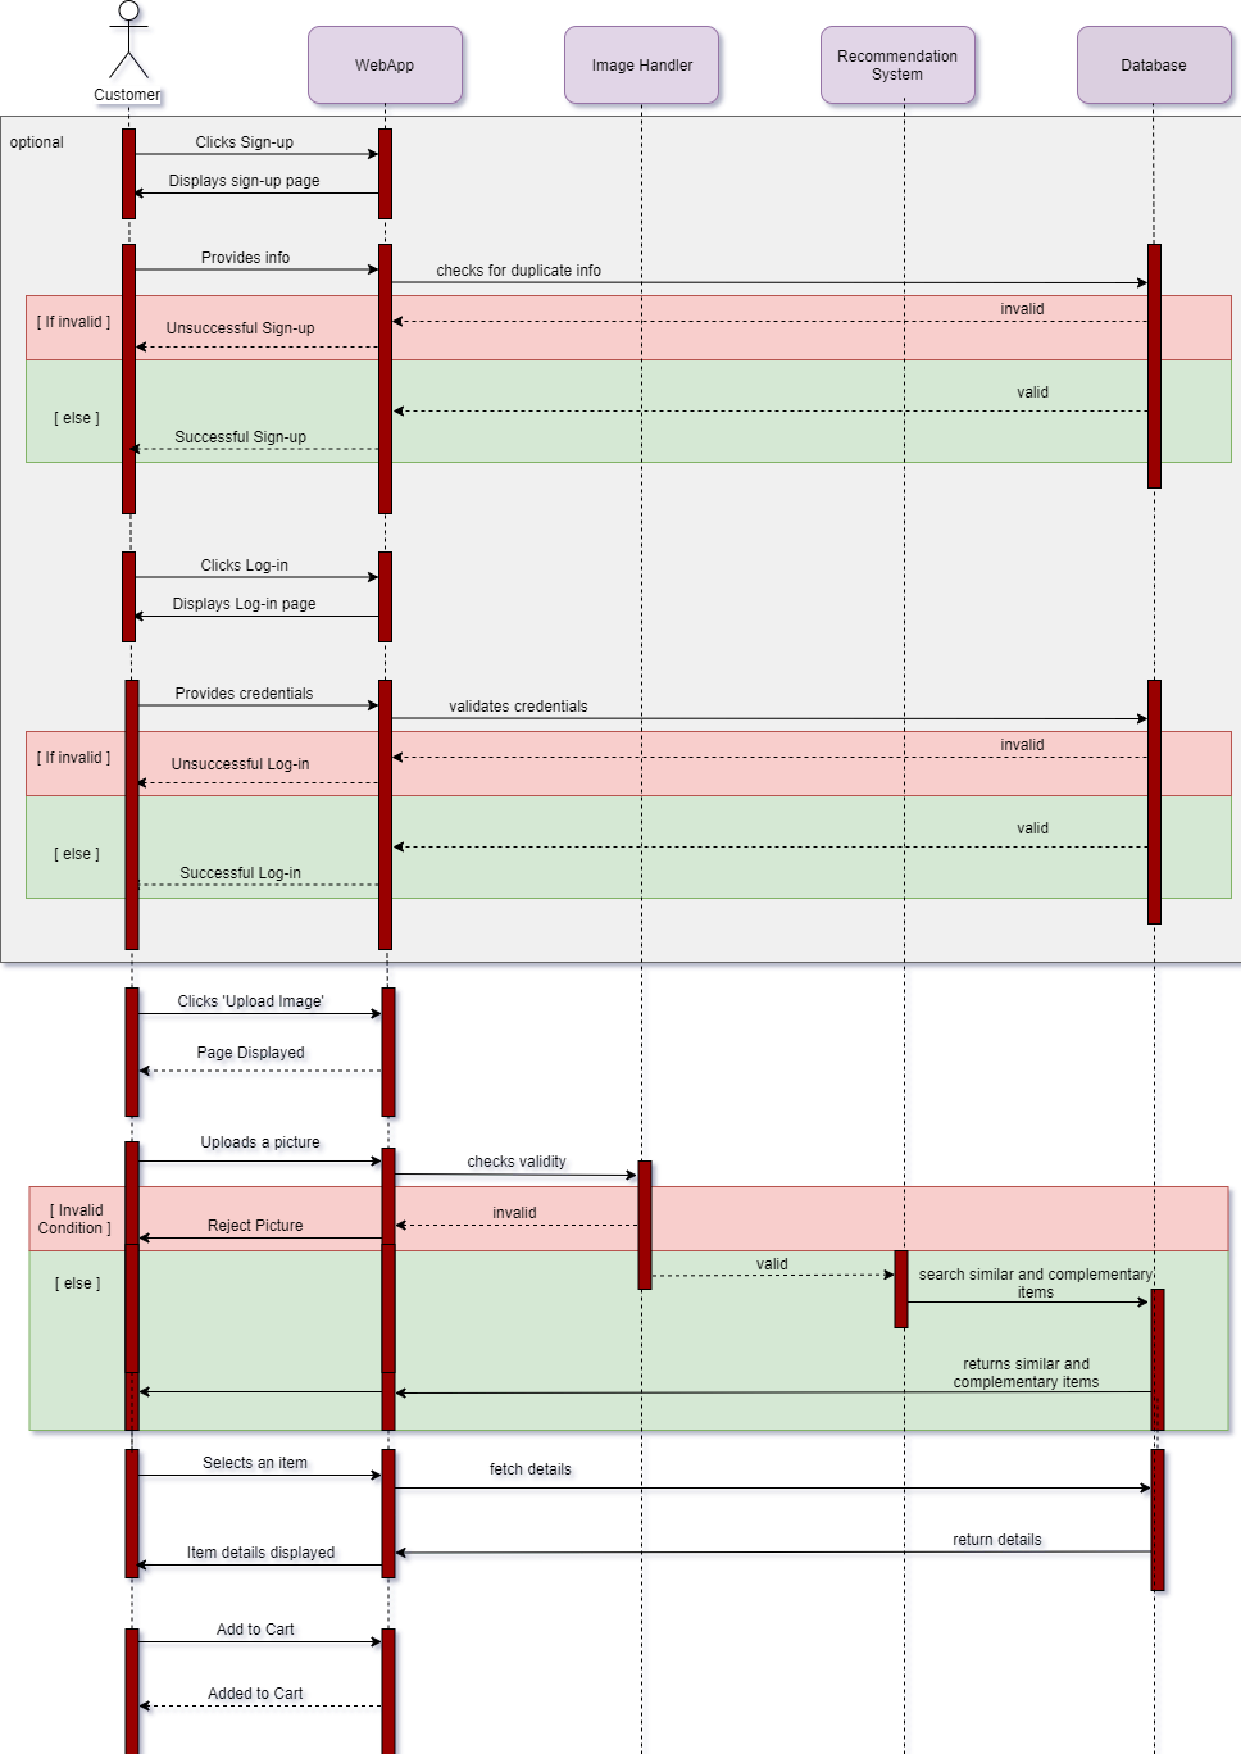
\includegraphics[width=12cm]{images/SequenceDiag1.pdf} 
\centering
\caption{Sequence Diagram - Customer}
\label{sequence: one}
\end{figure}

\chapter{Experiments and Results}
\label{chap:results}
The deep learning model that powers our recommendation systems visua'l search was iterated upon and consistently improved during the course of our Kaavish. We also made a concerted effort to ensure that our AI model was thoroughly tested and benchmarked at every experiment.

\begin{table}[H]
\begin{tabular}{ @{}|p{4cm}|p{5cm}|p{5cm}|  }
 \hline
 \multicolumn{3}{|c|}{\textbf{Experimentation- stages of evolution of the AI model}} \\
 \hline
 \textbf{Experiment. no} & \textbf{Number of Categories Trained On} & \textbf{Transfer Learning}\\
 
\hline
 1 & 20 & Yes \\ 
 \hline
 2 & 26 & Yes \\ 
 \hline
  3 & 50 & No \\
 \hline
\end{tabular}
\caption{Experimentation- stages of the AI model}
\label{table:Experimentation- stages of AI model}
\end{table}


Due to limitations in computing power, we initially trained the model on only the first 20 categories of the classification benchmark of the DeepFashion dataset. These categories correspond to the “top” clothing type (i.e. clothes worn on the top part of the body like shirts and coats, as opposed to items worn on the bottom like jeans). 

Once the viability of the model was proved in Kaavish I, we experimented by training our model on 26 categories that were selected based on their relevance to mens clothing, since that is the focus of our platform. Categories containing a large proportion of images of men's clothing were included while those containing a majority of women's clothing were excluded. 

The 26 categories included were: Anorak, Blazer, Bomber, Button-Down, Cardigan, Flannel, Henley, Hoodie, Jacket, Jersey, Parka, Peacoat, Sweater, Tank, Tee, Top, Turtleneck, Chinos, Jeans, Joggers, Shorts, Sweatpants, Sweat-shorts, Trunks, Coat and Robe. Other clothing categories such as blouse and skirt, which almost exclusively contained images of women, were excluded.

The motivation behind this experiment was to solve the problem of the lack of diversity in the subset of the DeepFashion dataset used to train the first model, which only contained items of the ``top" clothing type. By including only those categories we deemed to be relevant to a men’s fashion e-commerce store, we aimed to make our model more accurate while still minimizing computational cost. 

In the course of this experiment, we were provided access to Habib University’s new High Performance Computer, which contains an Nvidia Titan X GPU. With this significant increase in computational power at our disposal, we chose to train our model on all 50 categories of the DeepFashion dataset and so, no longer needed to complete the second experiment which we initially planned to carry out for Transfer learning. So its results are not available.

Although many of the newly included categories almost exclusively contain images of women’s clothing and no items in these categories are on our web application, our results showed that training on this additional data allowed our model to learn more meaningful features and improved its performance.

The availability of computational power also allowed us to train our model from scratch rather than use transfer learning, in which we would only train the last three layers of the model and all earlier layers were frozen with their weights set to the values obtained by training on the ImageNet dataset, accessed via the  \href{https://pytorch.org/docs/stable/torchvision}{torchvision package.} As noted in the above table, this provided a significant increase in performance but required the model to be trained for significantly longer before its performance stabilized (30 epochs versus 10 epochs).

All of these models were simultaneously trained on the classification and the in-shop retrieval benchmarks of the DeepFashion dataset respectively. The first model, which was trained on 20 categories of the classification benchmark was only trained on a subset of the in-shop retrieval benchmark corresponding to items of the ``top" clothing type. All other models were trained on multiple clothing types in the classification benchmark and so, were trained and tested on the entirety of the in-shop retrieval benchmark.

We also aimed to tune hyperparameters of our model for optimal performance by performing runs with different hyperparameter values and logging metrics such as loss and top-k accuracy using \href{https://www.tensorflow.org/tensorboard}{Tensorboard.} The following figures, which are screenshots from the Tensorboard dashboard, demonstrate how we used the tool to tune the learning rate by repeating training with different values of the learning rate and comparing performance across runs. Tensorboard logging also proved to be a valuable tool in monitoring the training of our models by observing their loss and \textit{top-$k$} accuracy on the train and test sets. Once the test accuracy of the model was seen to remain constant/decrease across multiple epochs, we terminated training and considered that run complete. 

\begin{figure}[H]
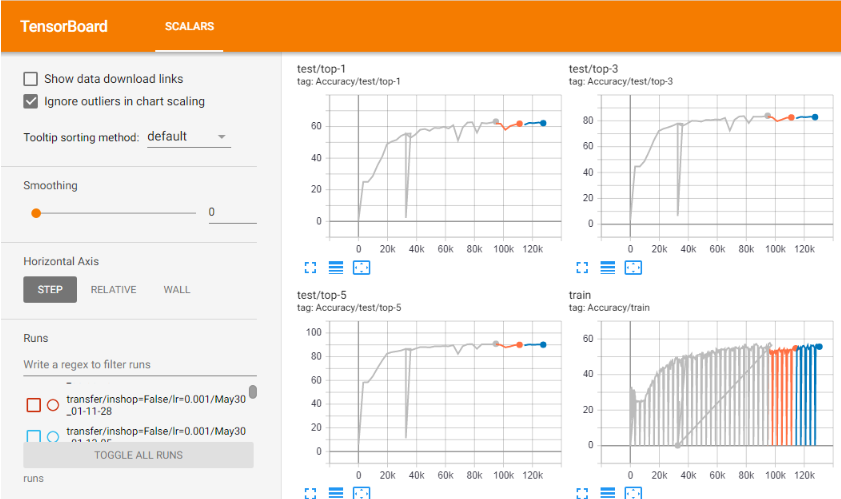
\includegraphics[width=15cm]{images/tensorboard.PNG} 
\centering
\caption{Logging model training of experiment \#3 with TensorBoard}
\label{architecture}
\end{figure}

The above figure shows the log of model training of the best model of the third experiment. The model was trained for a total of 40 epochs, which took 26 hours. The x-axis represents steps taken by the model (each step is one batch). The model was tested after every epoch. 

As expected, we see the test accuracy of the model increasing until it is almost constant. The model obtained after epoch 29 has the best test accuracy and so, is chosen as the best model. The train accuracy is logged after every 500 steps/batches, which explains the fluctuating nature of the ‘Accuracy/train’ graph. After applying smoothing to the graph, we see that the train accuracy is increasing with time, as expected. Note that the anomaly immediately before 40k steps is due to a power outage which interrupted training. 

Although our initial aim was to optimize our model by tuning as many hyperparameters as possible, this proved to be infeasible due to high training time of the model when it was trained and tested on the entirety of the DeepFashion classification and in-shop retrieval benchmarks due to the large size of the dataset. The classification benchmark contains 63,720 images while the in-shop retrieval benchmark contains a total of 54,642 images. Training the model for 40 epochs took approximately 26 hours. Hence, the optimization of hyperparameters has been left for future work. In this work we have trained with a small learning rate (0.001) to avoid overshooting optimal values and eliminate the need for hyper-parameter optimization. 

As we will discuss in the following section, the increase in performance that resulted from these experiments was significant in our benchmarks but the difference in real world retrieval results in our store proved to be minimal. So any further improvement obtained by tuning hyper-parameters would result in a negligible increase in the real world performance of the tool. This is because the catalog of our store is scrapped from local men’s e-commerce stores which have relatively small collections. We expect that with a larger and more diverse catalog, the increase in model performance would have translated to a more significant improvement in the real-world performance of the tool.\\

\section{Results}

The metrics used to test the performance of our models is the top-k accuracy in each respective task. For the classification task, we classify each image in the test set into one of the fifty categories. The classification is considered a success if the correct category label is among the top-k results of the model. Similarly, in-shop retrieval for an image in the test-query set is considered a success if on querying the test-gallery set, at least one of the top-k results is a photo of the same item.\newline

The results of our experiment are summarised in the table below for precised understanding and in order to ease the process of comparison between the results of different experiment conducted as part of the training of the recommendation system. The table is provided as follows:\\

\begin{table}[H]
\begin{tabular}{ @{}|p{2cm}|p{2cm}|p{2.75cm}|p{2.75cm}|p{2cm}|p{2cm}|  }
 \hline
 \multicolumn{6}{|c|}{\textbf{Results}} \\
 \hline
 \textbf{Model} & \textbf{Number of Categories Trained On} & \textbf{Classification top-3 Accuracy (\%)} & \textbf{Classification top-5 Accuracy (\%)}& \textbf{In-shop. top-5 Retrieval Accuracy (\%)}& \textbf{In-shop. top-20 Retrieval Accuracy (\%)}\\
 
  \hline
 Experiment \#1 & 20 & 87 & 95 & 74 & 86 \\ 
 \hline
 Experiment \#2 & 26 & N.A. & N.A. & N.A. & N.A. \\
 \hline
  Experiment \#3 & 50 & 84 & 91 & 81 & 91 \\
 \hline
 FashionNet (from DeepFashion research paper) & 50 & 82 & 90 & 68 & 76 \\
 \hline
\end{tabular}
\caption{Accuracy Comparison}
\label{table:ML experiment comparison}
\end{table}


As earlier mentioned, we received access to Habib University’s High Performance Computer while we were working on experiment #2. This significant  increase in computational power meant that we could train our model on all 50 categories to obtain a strictly superior result and no longer needed to train our model on 26 categories. Hence, experiment #2 was abandoned.

Note that since the model in experiment #1 is only trained on 20 categories (all of which belong to the ‘top’ clothing type), for the classification benchmark it is only tested on a subset of the test set containing only items of these 20 categories. Similarly, experiment #2 is only tested on 26 categories. For the in-shop retrieval benchmark, both are tested on the entire test set.

Our best model significantly outperforms FashionNet, the architecture proposed by the creators of the DeepFashion dataset, on the in-shop retrieval benchmark. Since this dataset and the accompanying FashionNet model were published in 2016, they no longer represent the state-of-the-art. These benchmarks show that our model performs extremely well and is more than adequate for this business problem.

\begin{figure}[H]
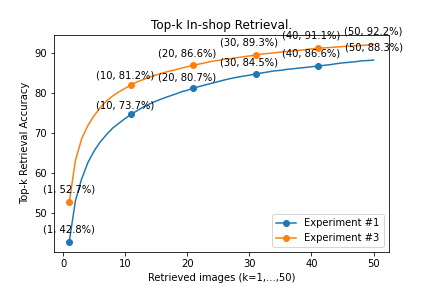
\includegraphics[width=12cm]{images/inshop-retrieval.png} 
\centering
\caption{Top-k in-shop accuracy of experiments 1 and 3.}
\label{architecture}
\end{figure}


Although, the increase in performance that resulted from these experiments was significant in our benchmarks but the difference in real world retrieval results in our store proved to be minimal. This is because the catalog of our store is scrapped from local men’s e-commerce stores which have relatively small collections. We expect that with a larger and more diverse catalog the increase in model performance would have translated to a more significant improvement in the real-world performance of the tool.

By matching the state-of-the-art in the field, we ensure that the performance of our model is not a limiting factor in taking this work forward and that it can be integrated into stores with larger and more complex catalogs while still performing more than adequately for this business scenario.

For the scope of this project, we do not believe that further optimization to our model (such as by tuning hyper-parameters or applying data augmentation) would yield any noticeable improvement in the tool’s real world performance and so, the tuning of hyper-parameters is left for future work.


\begin{figure}[H]
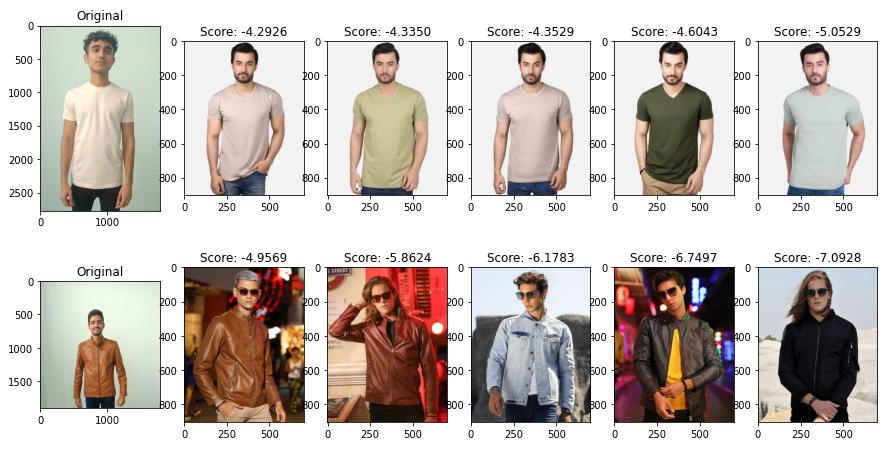
\includegraphics[width=12cm]{images/Recommendations1.PNG} 
\centering
\caption{Results of AI Model - Tops category}
\label{architecture}
\end{figure}

\begin{figure}[H]
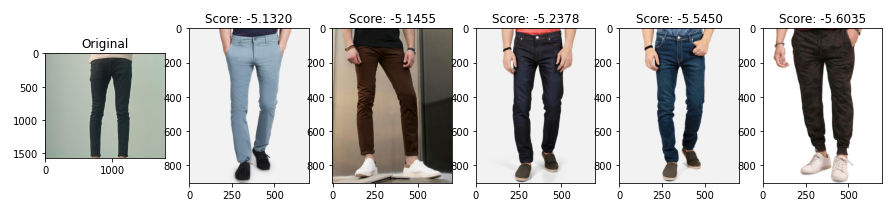
\includegraphics[width=12cm]{images/Recommendations2.PNG} 
\centering
\caption{Results of AI Model - Bottoms category}
\label{architecture}
\end{figure}

\begin{figure}[H]
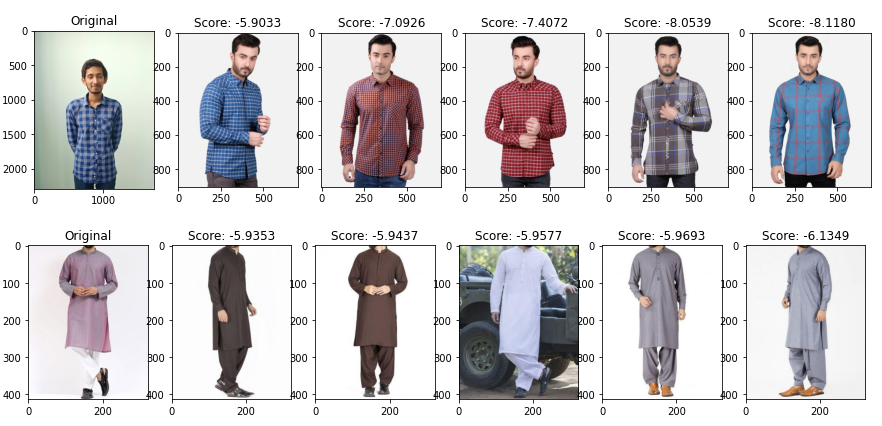
\includegraphics[width=12cm]{images/Recommendations3.PNG} 
\centering
\caption{Results of AI Model - Eastern Wear}
\label{architecture}
\end{figure}

\begin{figure}[H]
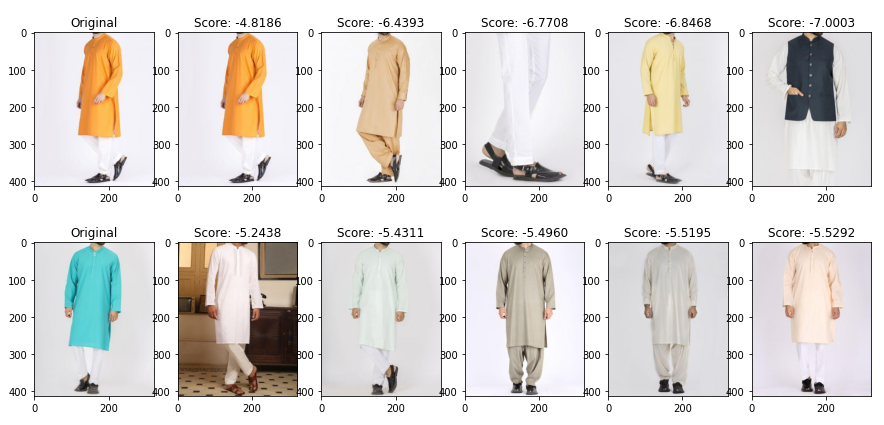
\includegraphics[width=12cm]{images/Recommendations4.PNG} 
\centering
\caption{Results of AI Model - Eastern Wear}
\label{architecture}
\end{figure}

\section{Complementary Recommendations}

We have successfully extended the functionality of our AI model to also recommend complementary items. When the user uploads an image, they receive two sets of recommendations: items that are visually similar and items that are visually complementary to the outfit in the uploaded image. Items are said to be complementary if they can be paired to create an outfit.

When a user uploads a query image, the model is run on it and two pieces of information are extracted to perform complementary item recommendation:
\begin{itemize}
    \item Predicted category of the item (t-shirt, jeans, hoodie etc.)
    \item Color vector- a set of 30 numbers that capture the color of the item
\end{itemize}

Based on the results of the category prediction by the model, a lookup table is then evaluated to find the categories of items that can be appropriately paired with it e.g. a t-shirt can not be paired with another t-shirt and hoodies and shorts are not generally worn together, so that combination is not recommended.

Currently, we have restricted the lookup table to the following 5 categories:

\begin{center}
\begin{tabular}{ |c|c| } 
 \hline
 \textbf{Category} & \textbf{Complementary Categories}\\
 \hline
T-shirt & Shorts, Jeans, Sweatpants, Hoodie, Jacket\\
 \hline
Button-down & Hoodie, Jacket, Jeans, Joggers, Sweatpants\\
 \hline
Jacket & Button-down, Sweater, T-shirt, Jeans, Sweatpants\\
 \hline
Jeans & Button-down, Sweater, Tee, Tank, Jacket\\
 \hline
 Eastern & Waistcoats\\
  \hline
\end{tabular}
\end{center}


In addition, the color vector is used to find the color of the outfit. This is done by comparing the vector to pre-computed color vectors of 10 solid colors and the closest matching color is found. The 10 colors that make up our database of solid colors can be seen in the following image.

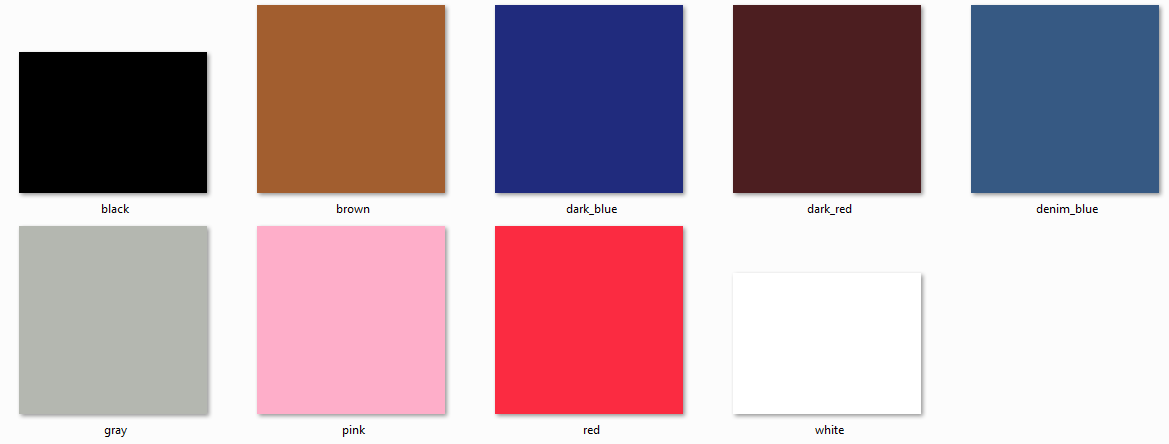
\includegraphics[scale=0.45]{colors.PNG}

A second lookup is then performed to find the colors that complement the color of the item. These color matching rules were created based on the outfits in our store which have been created.

The outputs of the clothing category compatibility and the color matching rules is used to fetch items that can be paired with the query item to create an outfit that is both appropriate and aesthetically appealing. The following are the snapshots of some of the outputs of the clothing category which are visually complimentary to the query image on the left. 

\begin{figure}[H]
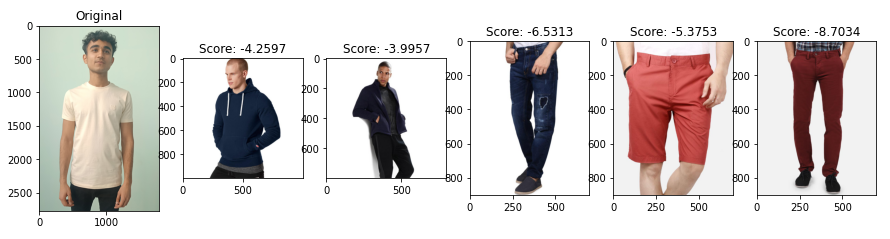
\includegraphics[width=12cm]{images/comp1.PNG} 
\centering
\caption{Results of AI Model for Complimentary Recommendation - Tops category}
\label{architecture}
\end{figure}

\begin{figure}[H]
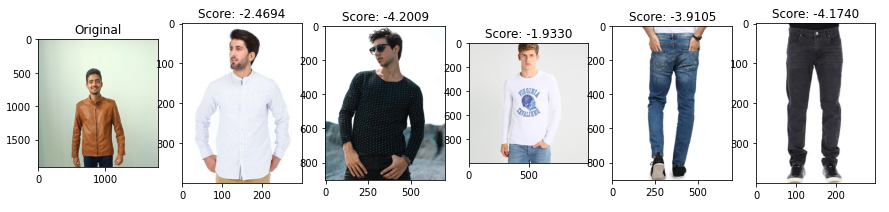
\includegraphics[width=12cm]{images/comp2.PNG} 
\centering
\caption{Results of AI Model for Complimentary Recommendations - Tops category}
\label{architecture}
\end{figure}

\begin{figure}[H]
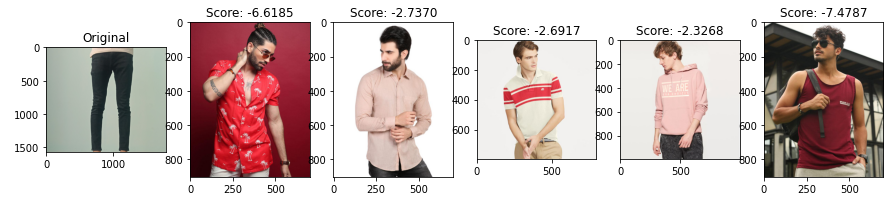
\includegraphics[width=12cm]{images/comp3.PNG} 
\centering
\caption{Results of AI Model for Complimentary Recommendations - Bottoms category}
\label{architecture}
\end{figure}

\begin{figure}[H]
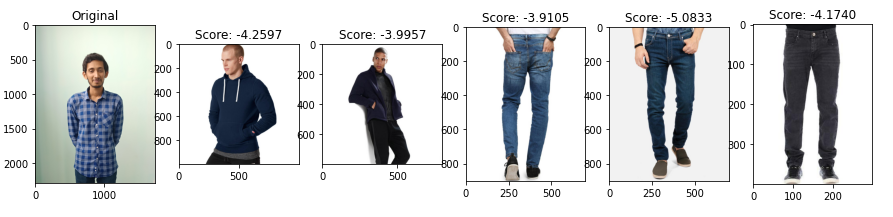
\includegraphics[width=12cm]{images/comp4.PNG} 
\centering
\caption{Results of AI Model for Complimentary Recommendations - Tops category (checked shirt)}
\label{architecture}
\end{figure}

\begin{figure}[H]
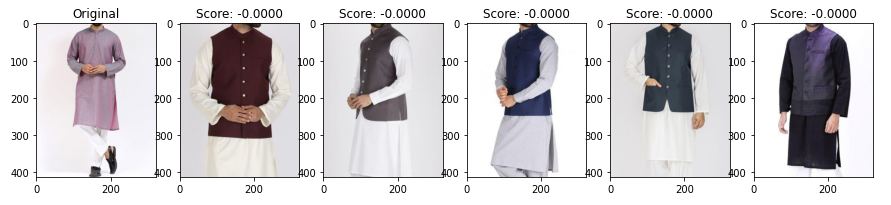
\includegraphics[width=12cm]{images/comp5.PNG} 
\centering
\caption{Results of AI Model for Complimentary Recommendations - Two-Piece category}
\label{architecture}
\end{figure}

\begin{figure}[H]
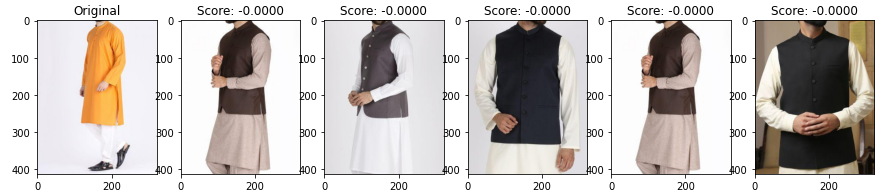
\includegraphics[width=12cm]{images/comp6.PNG} 
\centering
\caption{Results of AI Model for Complimentary Recommendations - Two-Piece category}
\label{architecture}
\end{figure}

\begin{figure}[H]
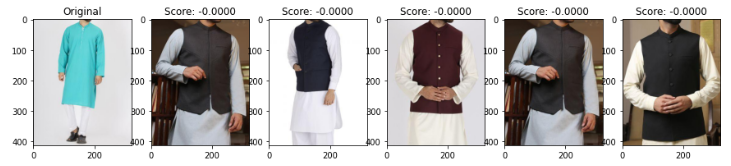
\includegraphics[width=12cm]{images/comp7.PNG} 
\centering
\caption{Results of AI Model for Complimentary Recommendations - Two-Piece category}
\label{architecture}
\end{figure}

\chapter{Conclusion and Future Work}
\label{chap:outro}
\section{Conclusion}

\section{Future Work}

In the future, first of all, we would look into the possibility to configure the recommendation model as a micro-service API and deploy the web application to a Web Server to make it feasible and accessible to both, the shoppers and the retailers.

Personalized Outfit Recommendation web application has a great potential to incorporate several enhancements in the future. Most importantly, refining the results of our AI model. Once the application is deployed and available publicly, there is a chance of collaborating with more local brands, meaning more data to feed into the AI model, consequently improving the recommendations. Additionally, the model will be trained in eastern fashion to make eastern recommendations more intelligent and robust, which is one of the novelties of this thesis. Furthermore, if the likes, dislikes, and purchase history of the customer are taken into account, it will further help to make the experience and recommendations more personalized for each customer. In addition to this, it can be further extended to the complete range of men's and women's clothing.

Lastly, a portable version of web application or a mobile application for Android and iOS would do a great deal in reaching out to a larger audience.

\begin{appendices}

\titleformat{\chapter}[hang]{\bf\huge}{Appendix \thechapter.}{2pc}{}
% \titleformat{\chapter}[hang]{\bf\huge}{\thechapter.}{2pc}{}

% This appendix is required if the data set is not fully described in the main text.
\chapter{Data}
Here is a dump of our 2TB data set. Enjoy!

% This appendix is required if the code is not fully described in the main text.
\chapter{Code}
% inspired by https://xkcd.com/221/
The entire code-base for all the modules - storefront, server, dashboard, this report, and the AI Model - can be found in \href{https://github.com/osama-usuf/Kaavish-II-PORS}{this consolidated GitHub repository}. Kaavish committee has already been given access to this private repository, and the codebase shall be made public for purposes of the evaluation and/or as per further instructions as given by the Kaavish committee.

The repository consists of all our work initiated and undertaken as part of the second part of our Kaavish module II. Detailed instructions on replicating the web application and a list of dependencies is also published there.

%%% Local Variables:
%%% mode: latex
%%% TeX-master: "../report"
%%% End:

\end{appendices}

% Print the bibliography with a ToC entry and titled, "References".
\printbibliography[heading=bibintoc,title={References}]

\end{document}

%%% Local Variables:
%%% mode: latex
%%% TeX-master: t
%%% End:
